
\documentclass[a4paper]{article}
\usepackage{subfig}
\usepackage{comment}
\usepackage{caption}
\usepackage{siunitx}%$[\si{\ohm}]$
\usepackage{array}
\usepackage{tabu}
\usepackage{float}
\usepackage{fancyhdr}
\usepackage{amsfonts}
\usepackage{amssymb}
\usepackage{indentfirst}
\usepackage{multirow}
\usepackage{multicol}
\usepackage{enumitem}
\usepackage{float}
\usepackage{amsmath}
\usepackage{listings}
\usepackage{color}
\usepackage{physics}
\usepackage{indentfirst}
\usepackage{enumitem}
\usepackage{mathrsfs}
\usepackage{tikz}
\usepackage[european]{circuitikz}	
\definecolor{codegreen}{rgb}{0,0.6,0}
\definecolor{codegray}{rgb}{0.5,0.5,0.5}
\definecolor{codepurple}{rgb}{0.58,0,0.82}
\definecolor{backcolour}{rgb}{0.95,0.95,0.92}
\lstdefinestyle{mystyle}{
    backgroundcolor=\color{backcolour},   
    commentstyle=\color{codegreen},
    keywordstyle=\color{magenta},
    numberstyle=\tiny\color{codegray},
    stringstyle=\color{codepurple},
    basicstyle=\footnotesize,
    breakatwhitespace=false,         
    breaklines=true,                 
    captionpos=b,                    
    keepspaces=true,                 
    numbers=left,                    
    numbersep=5pt,                  
    showspaces=false,                
    showstringspaces=false,
    showtabs=false,                  
    tabsize=2
}

\lstset{style=mystyle} %Revisar al final
\captionsetup[table]{skip=10pt}

%% Language and font encodings
\usepackage[spanish, es-tabla]{babel}
\usepackage[utf8x]{inputenc}
\usepackage[T1]{fontenc}

%% Sets page size and margins
\usepackage[a4paper,top=3cm,bottom=2cm,left=3cm,right=3cm,marginparwidth=1.75cm]{geometry}

%% Useful packages
\usepackage{amsmath}
\usepackage{graphicx}
%\graphicspath{./images} %Path
\usepackage[colorinlistoftodos]{todonotes}
\usepackage[colorlinks=true, allcolors=blue]{hyperref}

% Informacion portada
\pagestyle{fancy}
\fancyhf{}
\rhead{Procesamiento Digital de Señales y Aplicaciones}
\lhead{ELO313}
\rfoot{\thepage}

%%%%%%%%%%%%%%%%%%%%%% INICIO DOCUMENTO %%%%%%%%%%%%%%%%%%%%%%%%%%%%%%%%%%%%%
\begin{document}
% Portada
\begin{titlepage}
	\centering
	{\scshape\LARGE [ELO313] Procesamiento Digital de Señales y Aplicaciones\par}
	\vspace{1cm}
	{\scshape\Large Tarea $\#1$\par}
	\vspace{5cm}	
	{\huge\bfseries Sistemas y correlación en tiempo discreto \par}
	\vspace{9cm}
	{\Large\Large Mauricio Aravena Cifuentes \\ 201503001-4}
	\vfill
	{\large \ \today \par}
\end{titlepage}
% Informe
\section{Evaluación de propiedades de sistemas}
	Para evaluar las propiedades de los siguientes sistemas, se utilizaron las siguientes señales, de acuerdo al criterio que se buscaba evaluar:
	\begin{itemize}
		\item \textbf{Invariancia temporal:} Se utilizó un pulso cuadrado, de duración 1 \textit{s}, con amplitud 1. Luego se utiliza un pulso de las mismas características pero retrasado temporalmente en $k = 5$\textit{s}. En el caso de que ambas entradas, lleguen a la misma salida, únicamente retrasadas, el sistema es invariante en el tiempo.
		\begin{equation}
			y[n-k] = S\{ x[n-k]  \}
			\label{eq:cond_invarianza_temporal}
		\end{equation}
		
		\item \textbf{Linealidad:} Se utilizan, dos señales de ruido blanco de potencia 10 dB, las cuales se amplifican por constantes $\alpha$ y $\beta$. De esta manera, luego se aplica la definición de sistemas lineales para comprobar:
		\begin{equation}
			\alpha y_{1}[n] + \beta y_{2}[n] = S \{ \alpha x_{1}[n] + \beta x_{2}[n] \} 
			\label{eq:cond_linealidad}
		\end{equation}
		
		De esta forma, si el sistema cumple ambos lado de la igualdad, se tendrá que el sistema es lineal. Para los siguientes sistemas, se escogieron los siguientes valores para las variables:
		\begin{table}[H]
			\center
			\begin{tabular}{|c|c|}
				\hline
				\textbf{Constante} & \textbf{Valor} \\
				\hline
				$\alpha$ & 2 \\
				\hline
				$\beta$ & 3 \\
				\hline			
			\end{tabular}
			\caption{Valores para constantes para probar linealidad}
			\label{tab:lineal_const_values} 	
		\end{table}
		
		Para simplificar la notación, en los gráficos de prueba, se denomina a las entradas de ruido blanco escaladas de la siguiente forma:
		\begin{align}
			u_{1}[n] = \alpha x_{1}[n] \\
			u_{2}[n] = \beta x_{2}[n]
			\label{eq:lineality_inputs}
		\end{align}
		
		También se define las salidas esperadas, dadas la expresión en la ecuación \ref{eq:cond_linealidad}, de la siguiente manera: 
		\begin{equation*}
			\underbrace{\alpha y_{1}[n] + \beta y_{2}[n]}_{Y_{1}[n] + Y_{2}[n]} = \underbrace{S \{ \alpha x_{1}[n] + \beta x_{2}[n] \}}_{Y[n]} 
		\end{equation*}
		De esta forma, llegando a expresiones más compactas, en términos de lo que se obtuvo en matlab:
		\begin{align}
			Y[n] = S \{ u_{1}[n] + u_{2}[n] \} \\
			Y_{1}[n] = S \{ u_{1}[n] \} \\
			Y_{2}[n] = S \{ u_{2}[n] \}
			\label{eq:lineality_outputs}
		\end{align}
		
		\item \textbf{Estabilidad BIBO:} Para comprobar esta propiedad, se utiliza un delta de Kronecker, un escalón unitario  y una señal triangular de frecuencia 1 \textit{Hz}. Luego analizamos la respuesta del sistema, utilizando la siguiente definición:
		\begin{equation}
			|x[n]| \leq M_{x} < \infty \Rightarrow |y[n]| \leq M_{y} < \infty \quad \forall n
			\label{eq:cond_bibo}
		\end{equation}
		
		De esta forma, analizamos la salida del sistema frente a las entradas, y se busca comprobar que ésta sea acotada.  
	\end{itemize}

\newpage

	\subsection{Sistema \#1}
		\subsubsection{Invariancia temporal}
			Aplicando la señal de prueba en el sistema, con retardo igual a cero:
			\begin{figure}[H]
				\center
				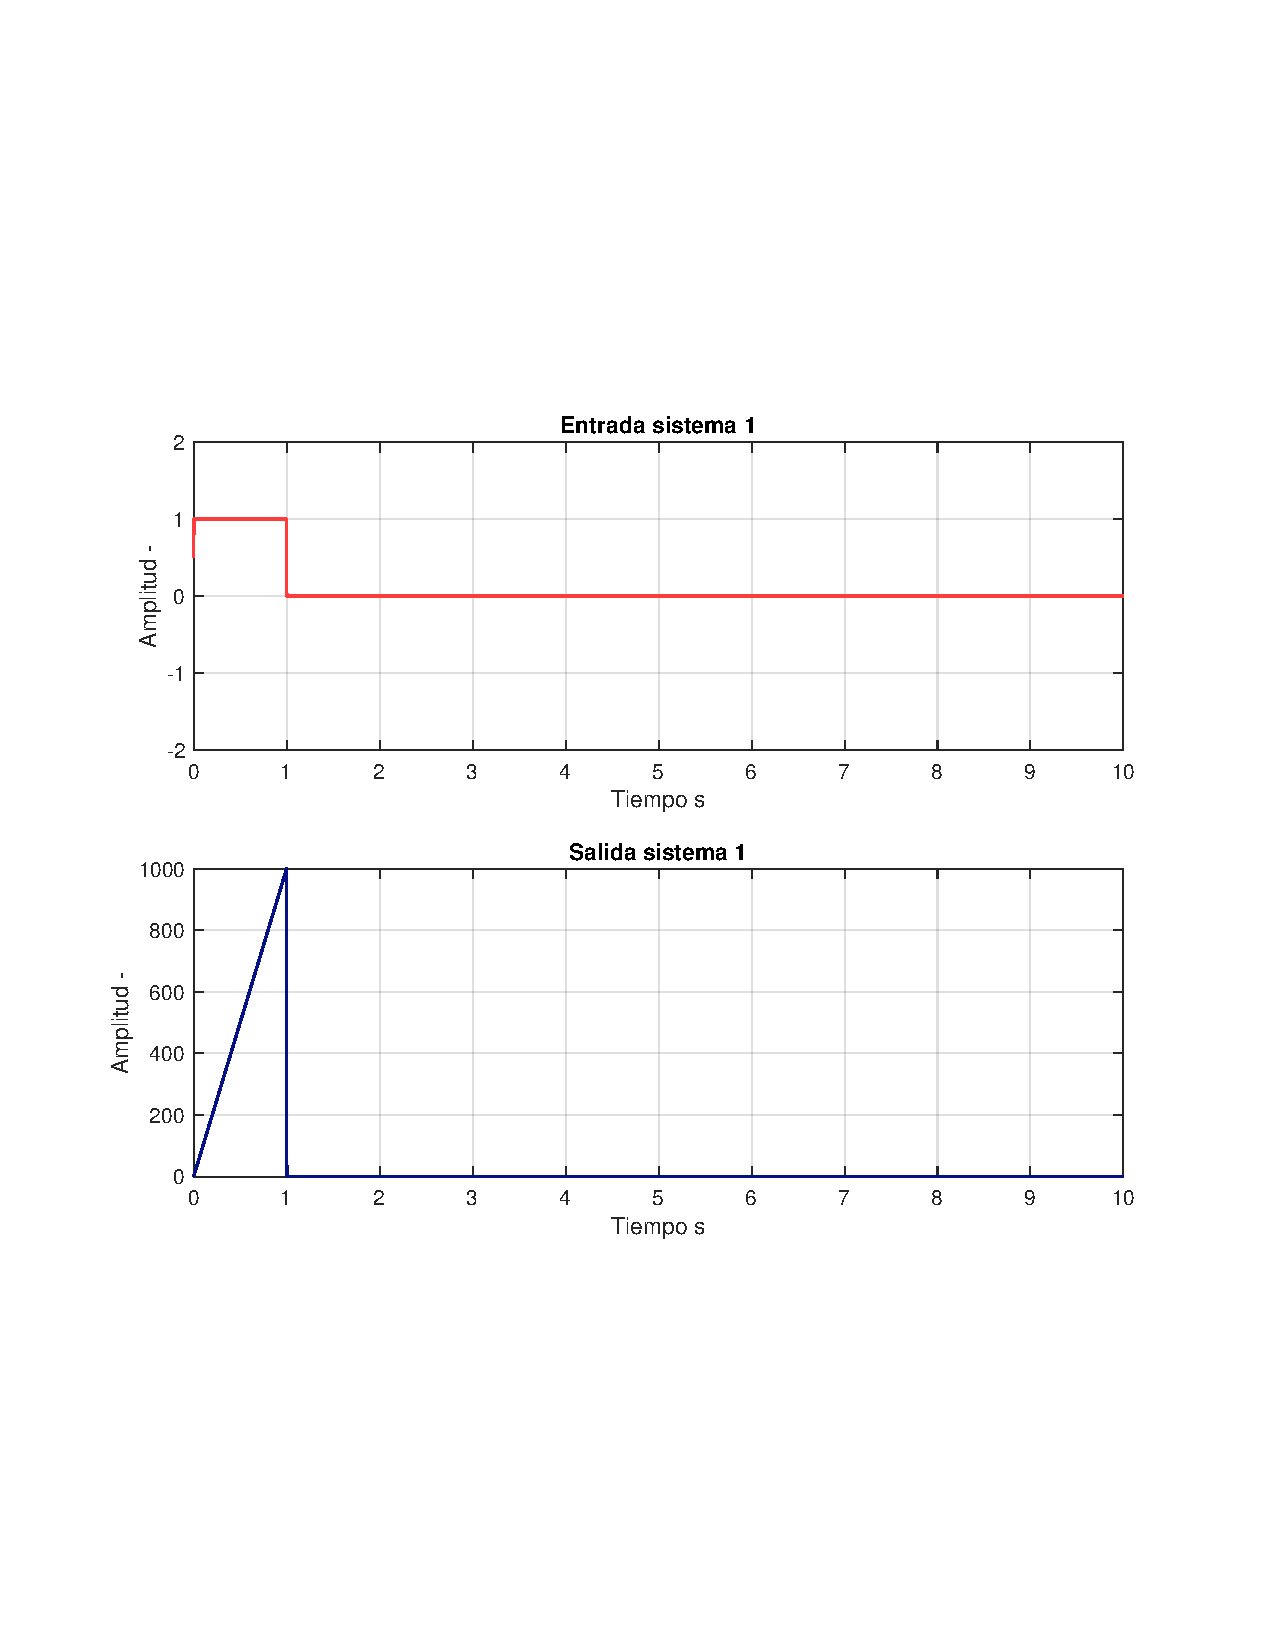
\includegraphics[width=0.6\textwidth,clip, trim = {2cm 7.0cm 2.2cm 7.0cm}]{../imgs/sistema_1_invarianza_temporal_noretardo.pdf}
				\caption{Sistema \#1 Entrada: Pulso cuadrado, de duración 1 \textit{s} \textbf{(Arriba)}. Salida del sistema \textbf{(Abajo)}.}
				\label{fig:s_1_time_invariant_test_1}
			\end{figure}
			
			Generando un retardo para la señal de entrada, equivalente a 5 \textit{s}, se obtiene:
			
			\begin{figure}[H]
				\center
				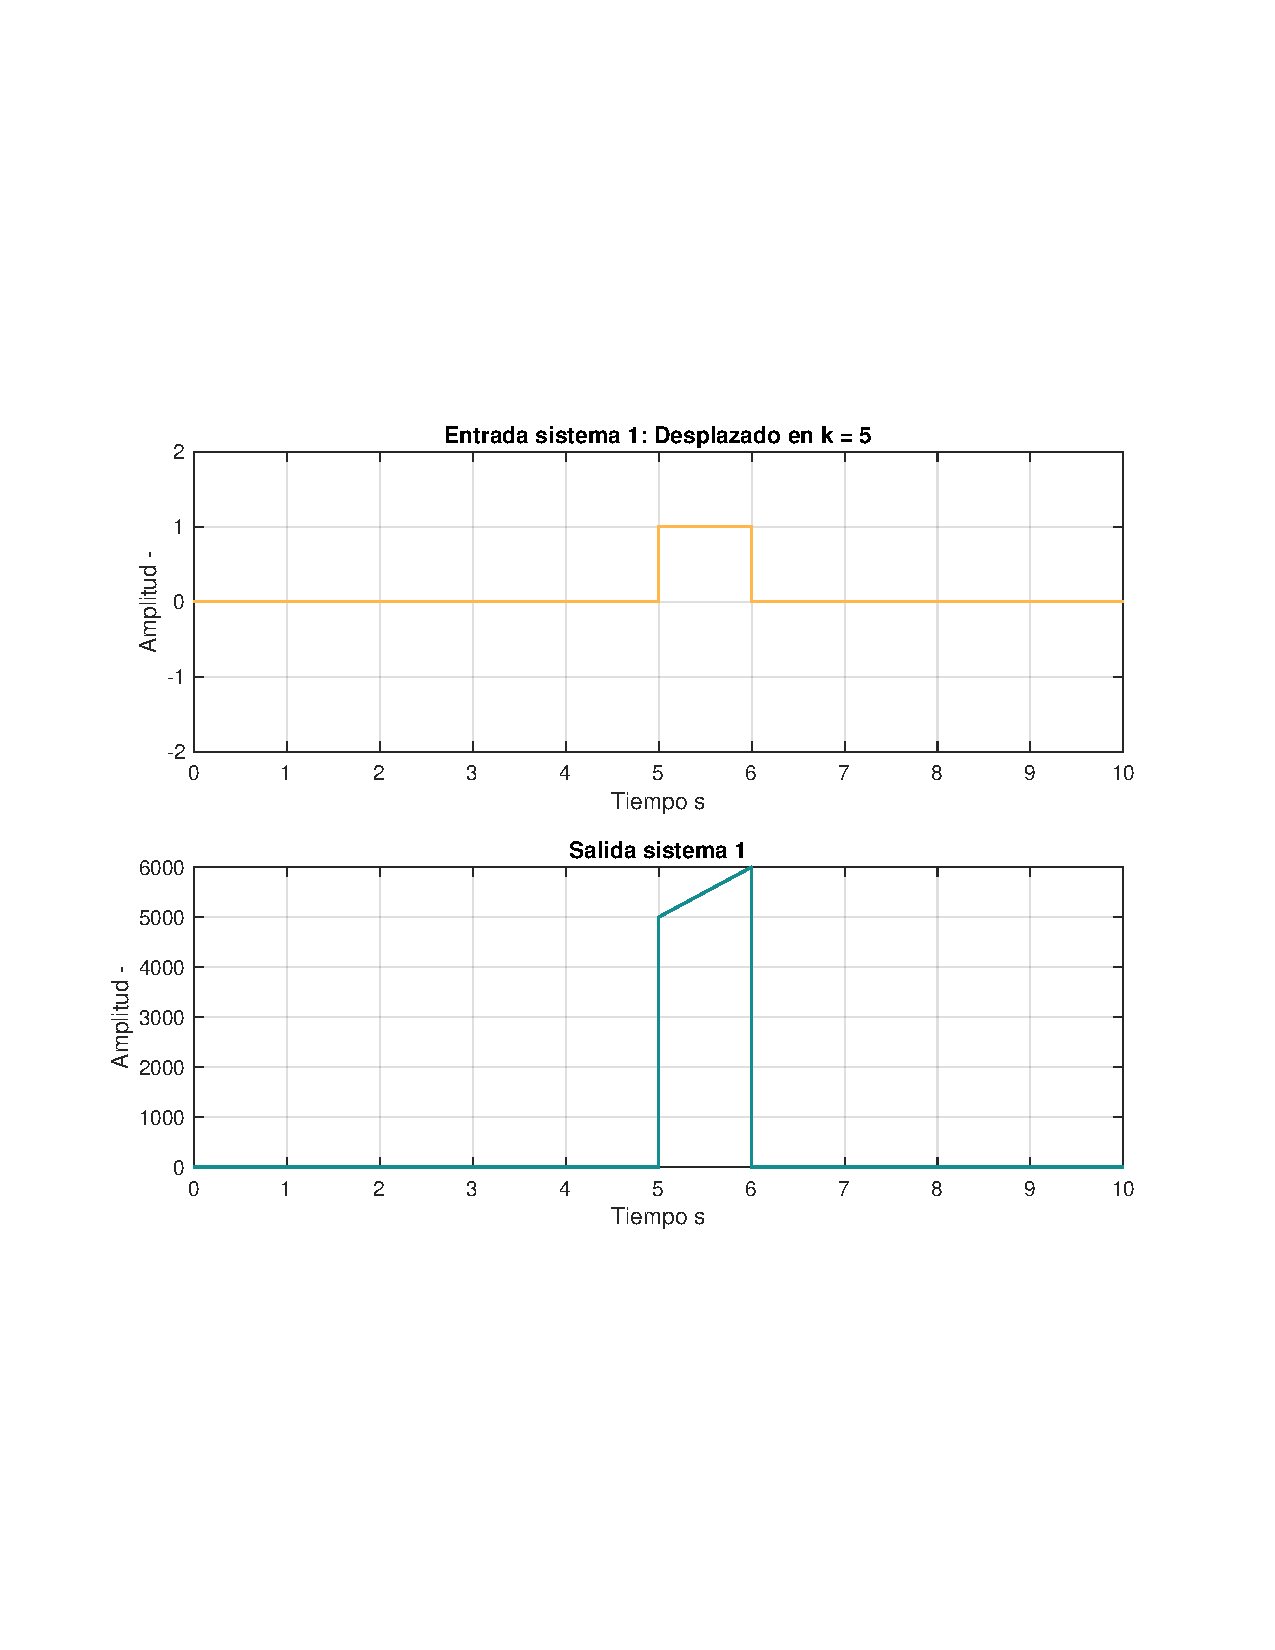
\includegraphics[width=0.6\textwidth,clip, trim = {2cm 7.0cm 2.2cm 7.0cm}]{../imgs/sistema_1_invarianza_temporal_retardo.pdf}
				\caption{Sistema \#1 Entrada: Pulso cuadrado de duración 1 \textit{s}, con un retardo de 5 \textit{s} \textbf{Arriba}.Salida del sistema \textbf{Abajo}.}
				\label{fig:s_1_time_invariant_test_2}
			\end{figure}
			
			A partir de los resultados, claramente el sistema es \textbf{variante en el tiempo}, dado que la señal de entrada retardada no equivale a la señal de salida retardada, no cumpliendo la definición de un sistema invariante según ecuación \ref{eq:cond_invarianza_temporal}.

\newpage

		\subsubsection{Linealidad}
			Se generaron las entradas del sistema, $u_{1}[n]$ y $u_{2}[n]$: 
			\begin{figure}[H]
				\center
				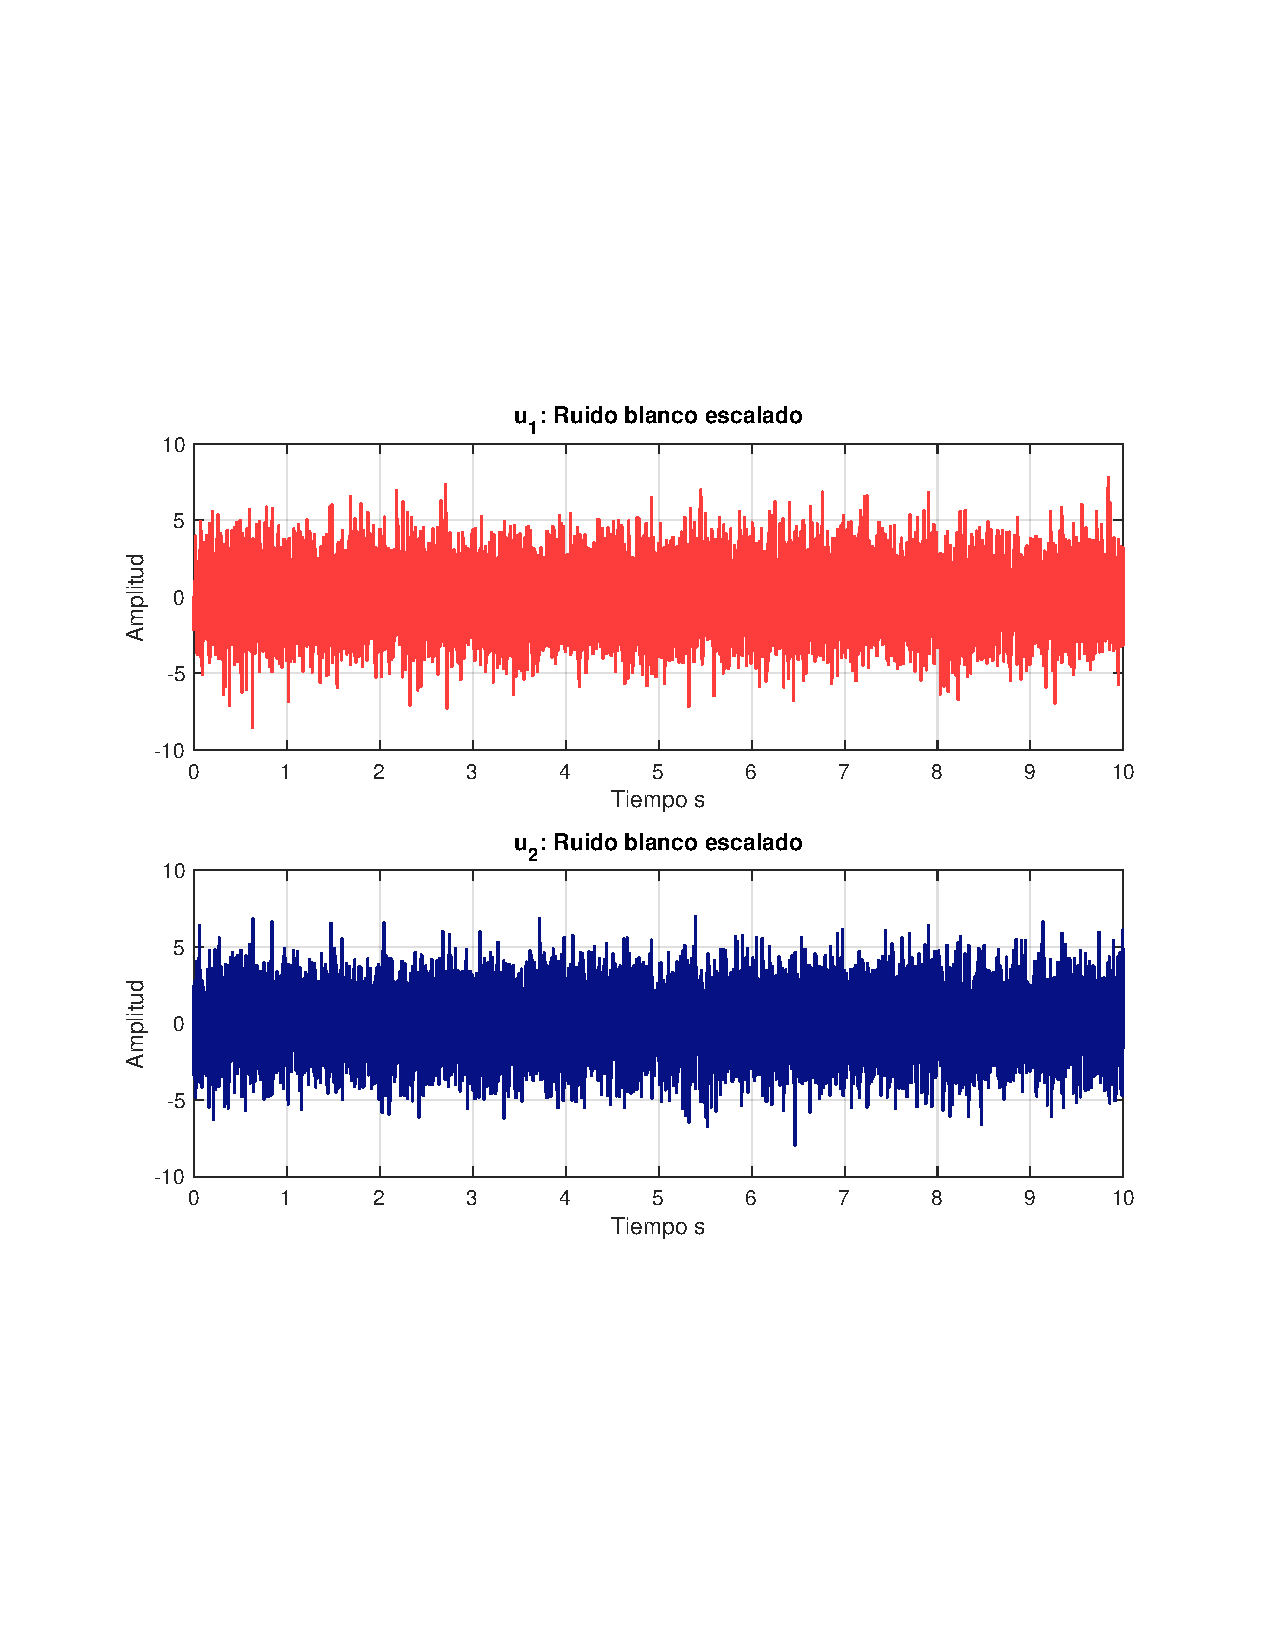
\includegraphics[width=0.6\textwidth,clip, trim = {2cm 7.0cm 2.2cm 7.0cm}]{../imgs/sistema_1_linealidad_entradas.pdf}
				\caption{Entradas del sistema}
				\label{fig:s_1_lineality_inputs}
			\end{figure}

			Para comprobar la linealidad, se necesita que la ecuación \ref{eq:cond_linealidad} se cumpla tanto a su lado izquierdo como derecho, por lo que se genero los términos correspondientes a ambos lados, utilizando la notación dada por la expresión \ref{eq:lineality_outputs}:
			
			\begin{figure}[H]
				\center
				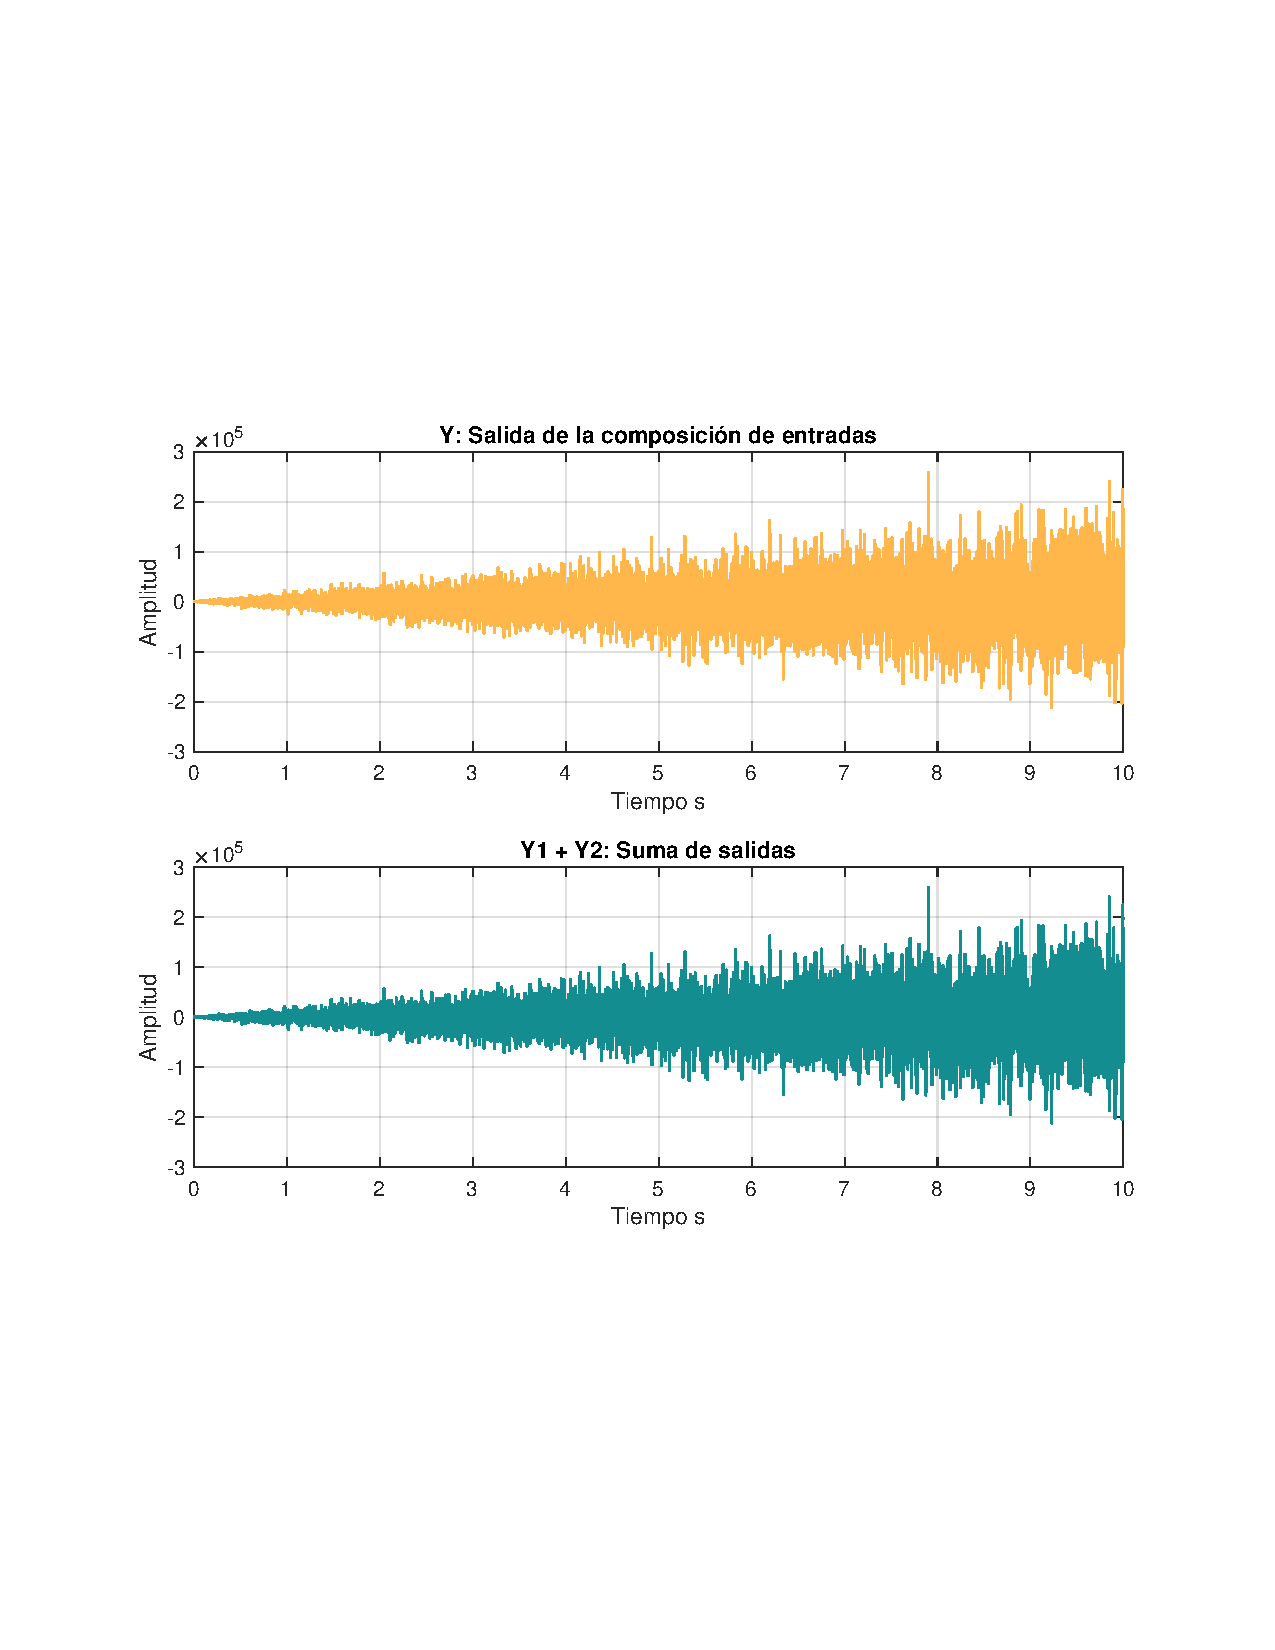
\includegraphics[width=0.6\textwidth,clip, trim = {2cm 7.0cm 2.2cm 7.0cm}]{../imgs/sistema_1_linealidad_salidas.pdf}
				\caption{Salidas del sistema: $Y[n]$ \textbf{(Arriba)}. $Y_{1}[n] + Y_{2}[n]$ \textbf{(Abajo)}.}
				\label{fig:s_1_lineality_outputs}
			\end{figure}
			
			A simple vista, se puede especular que el sistema se comporta de manera lineal, para comprobar esta aseveración, se superpondrá una señal sobre la otra y se calculará la diferencia entre ambas:
			\begin{figure}[H]
				\center
				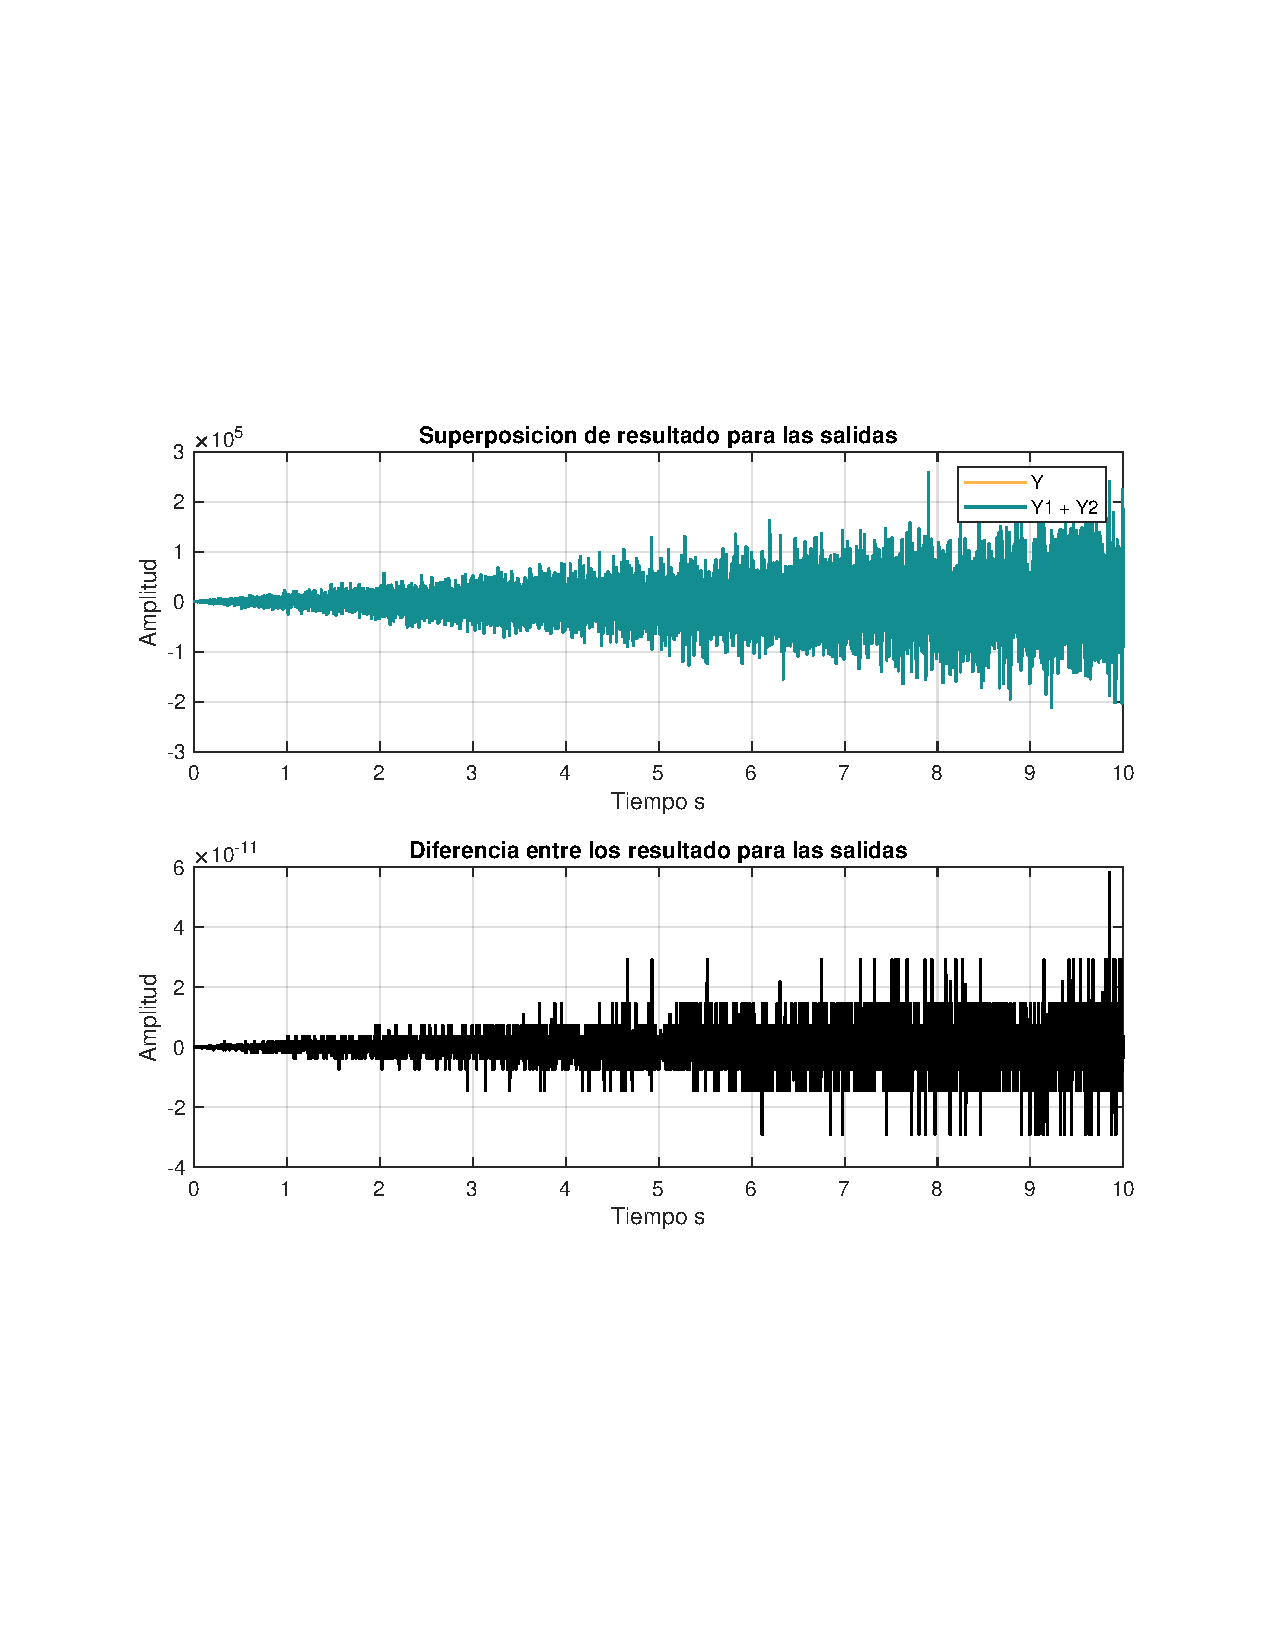
\includegraphics[width=0.6\textwidth,clip, trim = {2cm 7.0cm 2.2cm 7.0cm}]{../imgs/sistema_1_linealidad_superpuestas.pdf}
				\caption{Superposición de las señales de salida \textbf{(Arriba)}. Representación de la resta punto a punto de las señales. \textbf{(Abajo)}.}
				\label{fig:s_1_lineality_superposition}
			\end{figure}
			
			Como se puede observar en la parte superior de la Figura \ref{fig:s_1_lineality_superposition}, ambas señales son iguales, lo que se puede comprobar en la parte inferior de la misma figura, que representa la diferencia:
			\begin{equation*}
				Y [n] -  \left( Y_{1} [n] + Y_{2}[n] \right) 
			\end{equation*}
			
			Dado, que esta está en el orden de $10^{-11}$ se puede concluir que ambas señales son iguales, por lo tanto el sistema es \textbf{lineal}.\footnote{Esta diferencia se puede atribuir a redondeos en tiempo de ejecución realizados por el programa al evaluar las entradas en el sistema}
			
		\subsubsection{Estabilidad BIBO}
			Aplicando como señal de entrada, un delta de Kronecker: 
			\begin{figure}[H]
				\center
				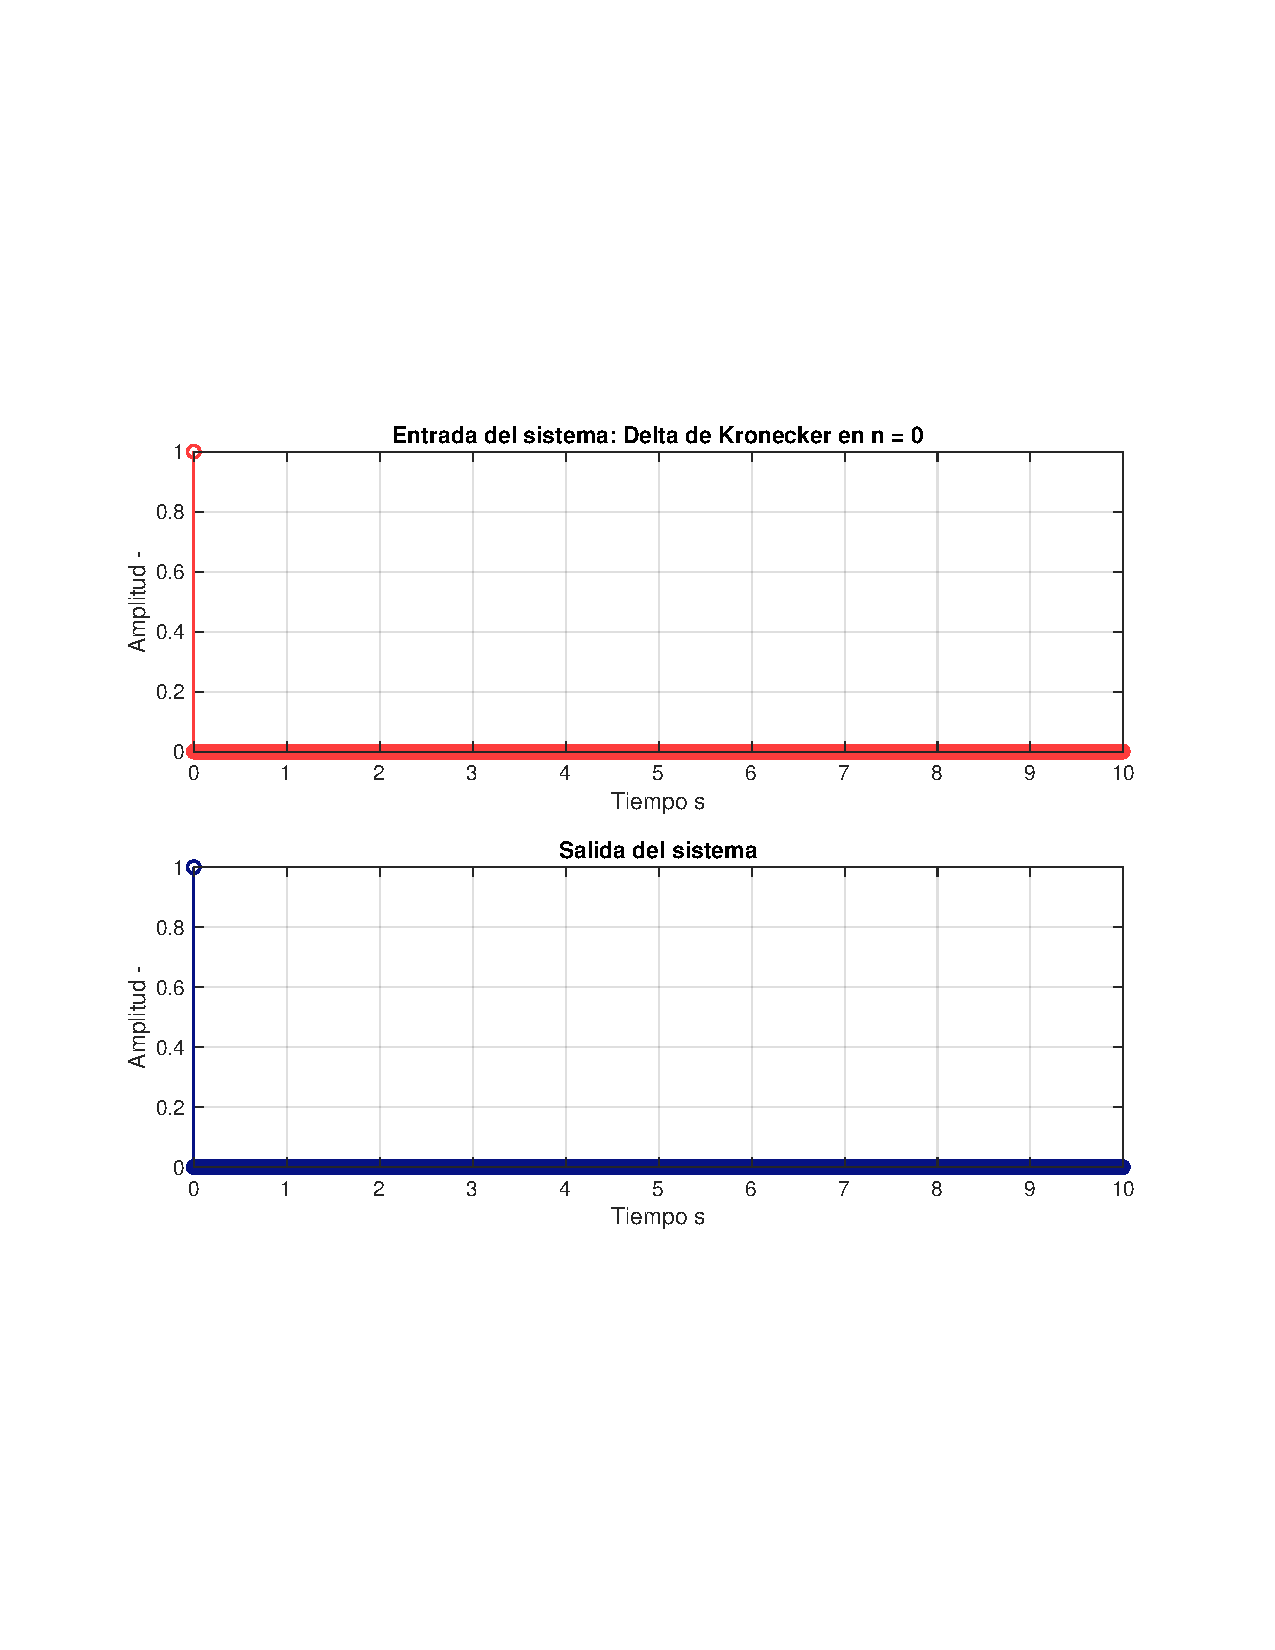
\includegraphics[width=0.6\textwidth,clip, trim = {2cm 7.0cm 2.2cm 7.0cm}]{../imgs/sistema_1_bibo_n_0.pdf}
				\caption{Sistema \#1, para una entrada de un delta de Kronecker \textbf{(arriba)}, se tiene la siguiente respuesta \textbf{(abajo)}.}
				\label{fig:s_1_bibo_0}
			\end{figure}
			
			Notemos, que el resultado, no es de mucha información dado que considerando únicamente esto, podríamos decir que el sistema se comportaria de forma estable. Sin embargo, modificando la entrada para que ahora tenga un retardo de $n = 50$ muestras:
			\begin{figure}[H]
				\center
				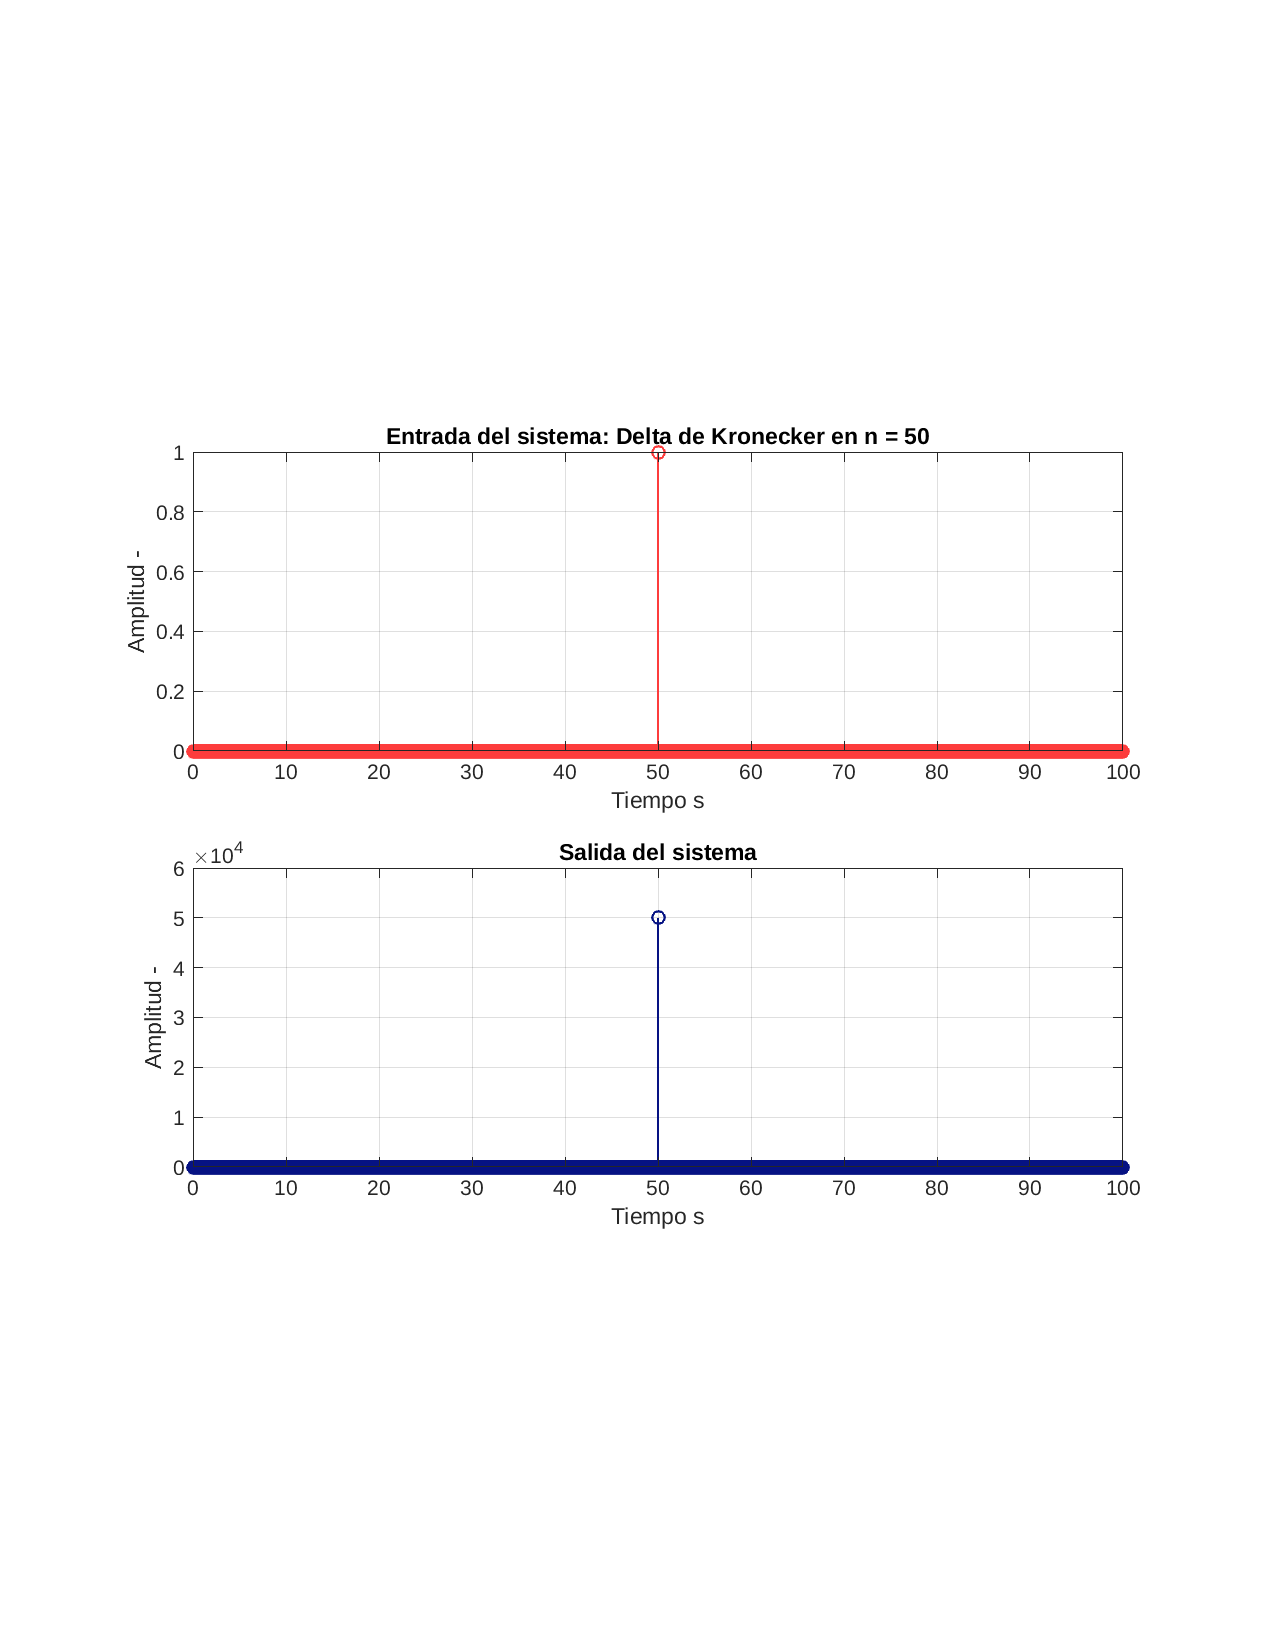
\includegraphics[width=0.6\textwidth,clip, trim = {2cm 7.0cm 2.2cm 7.0cm}]{../imgs/sistema_1_bibo_n_50.pdf}
				\caption{Sistema \#1, para un delta de Kronecker desplazado 50 muestras a la derecha \textbf{(arriba)}. Salida del sistema \textbf{(abajo)}.}
				\label{fig:s_1_bibo_50}
			\end{figure}
			
			Notemos que ahora, se tiene una señal similar a la obtenida en figura \ref{fig:s_1_bibo_0}, sin embargo, ahora el delta que se obtiene a la salida está amplificado por un facotor de ~ $5 \cdot 10^{4}$, esto es debido a que el sistema se comporta como un amplificador, dependiente el tiempo. A medida que avanza el tiempo, la amplificación aumenta:
			\begin{figure}[H]
				\center
				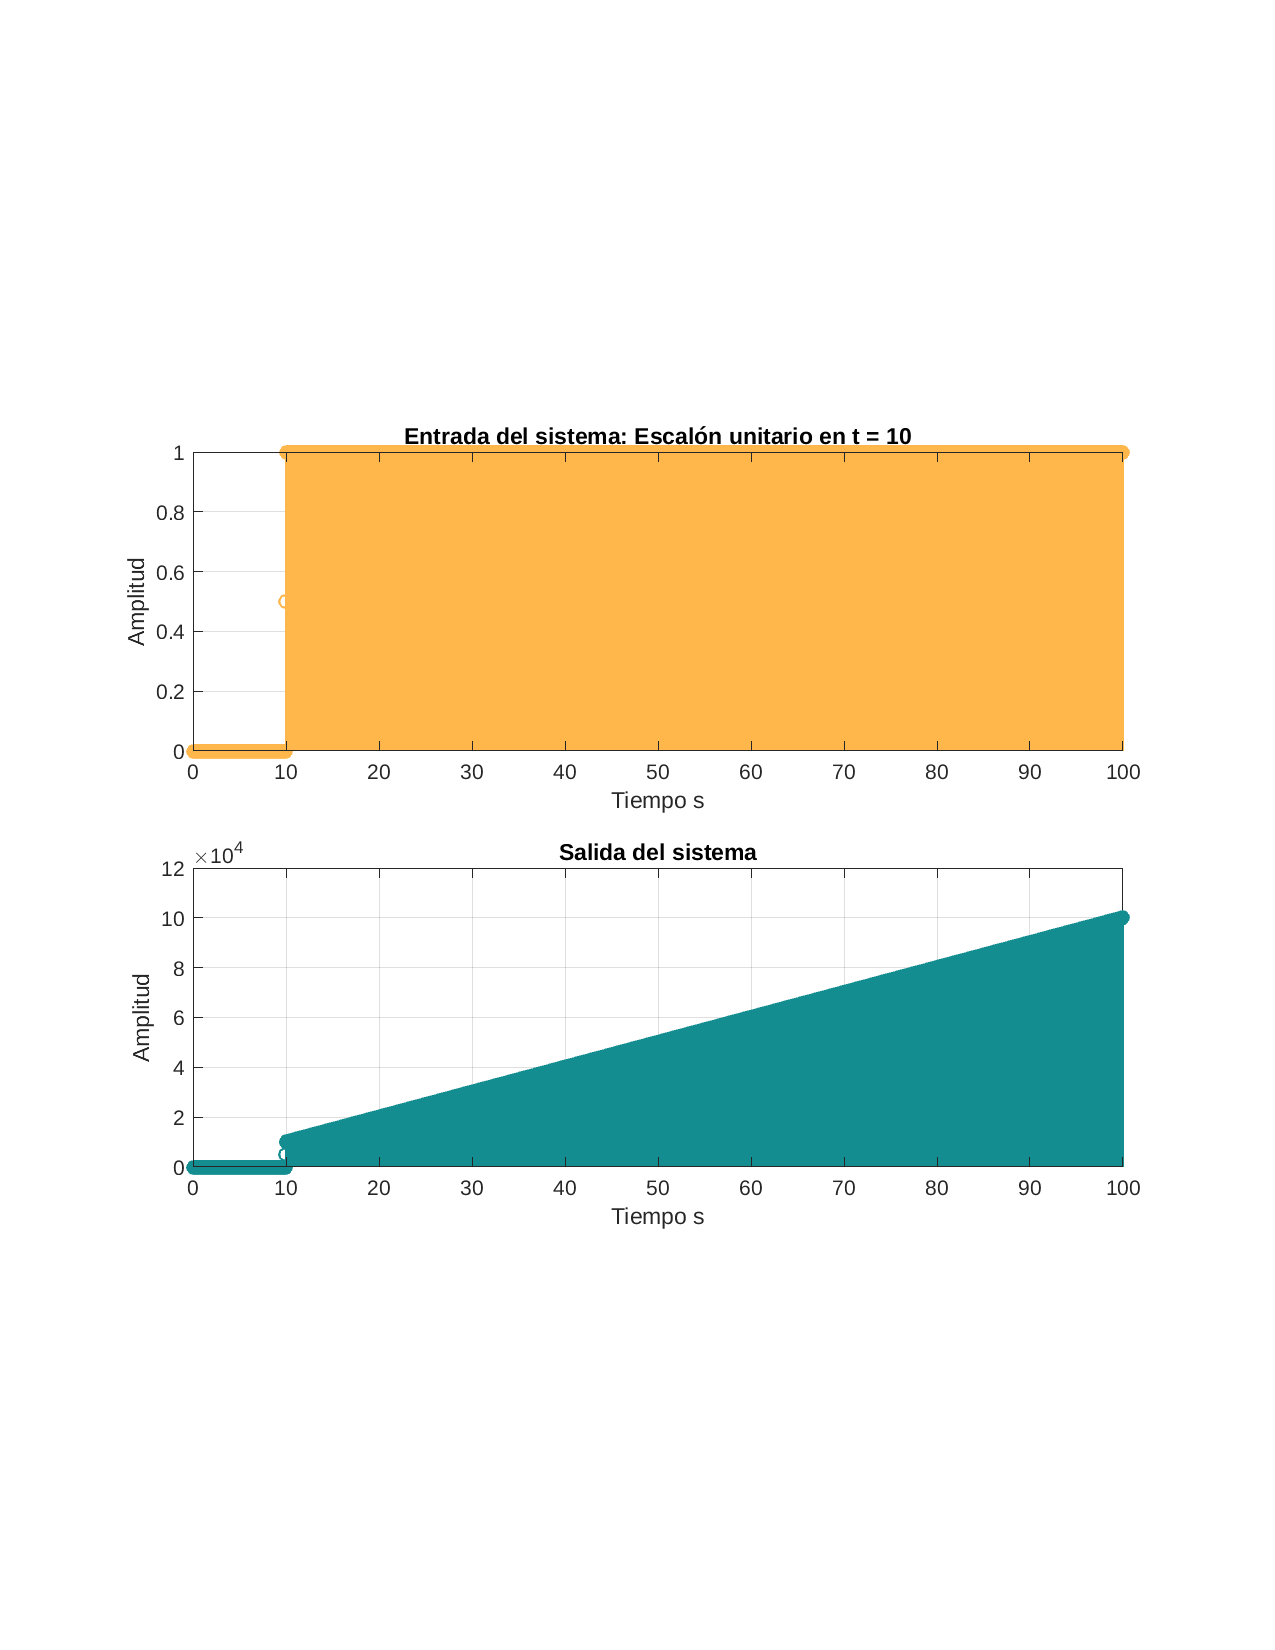
\includegraphics[width=0.6\textwidth,clip, trim = {2cm 7.0cm 2.2cm 7.0cm}]{../imgs/sistema_1_bibo_step.pdf}
				\caption{Sistema \#1, para una escalón unitario, activado en t = 10 \textbf{(arriba)}. Salida del sistema \textbf{(abajo)}.}
				\label{fig:s_1_bibo_step}
			\end{figure}
			
			Como se puede apreciar, a medida que pasa el tiempo, la señal tiende a amplificarse, por lo que se puede especular que si se toma un tiempo muy grande y muestras acorde a este tiempo:
			\begin{equation}
			\lim_{k \rightarrow \infty}  S\{ x[n -k] \} \rightarrow \infty  
			\end{equation}
			
			Dado, que a medida que pasa el tiempo, la amplificación sobre la señal de entrada aumenta, por lo que independiente que $x[n-k]$ sea una señal acotada, la salida del sistema tenderá a infinito. Por lo que podemos especular que el sistema es \textbf{inestable}.\footnote{Note que no es necesario probar con otras señales, dado que ya se comprobó que el sistema es inestable.}
			
\newpage

		\subsection{Sistema \#2}
			\subsubsection{Invariancia temporal}
				Aplicando la señal de prueba en el sistema, con retardo igual a cero:
				\begin{figure}[H]
				\center
				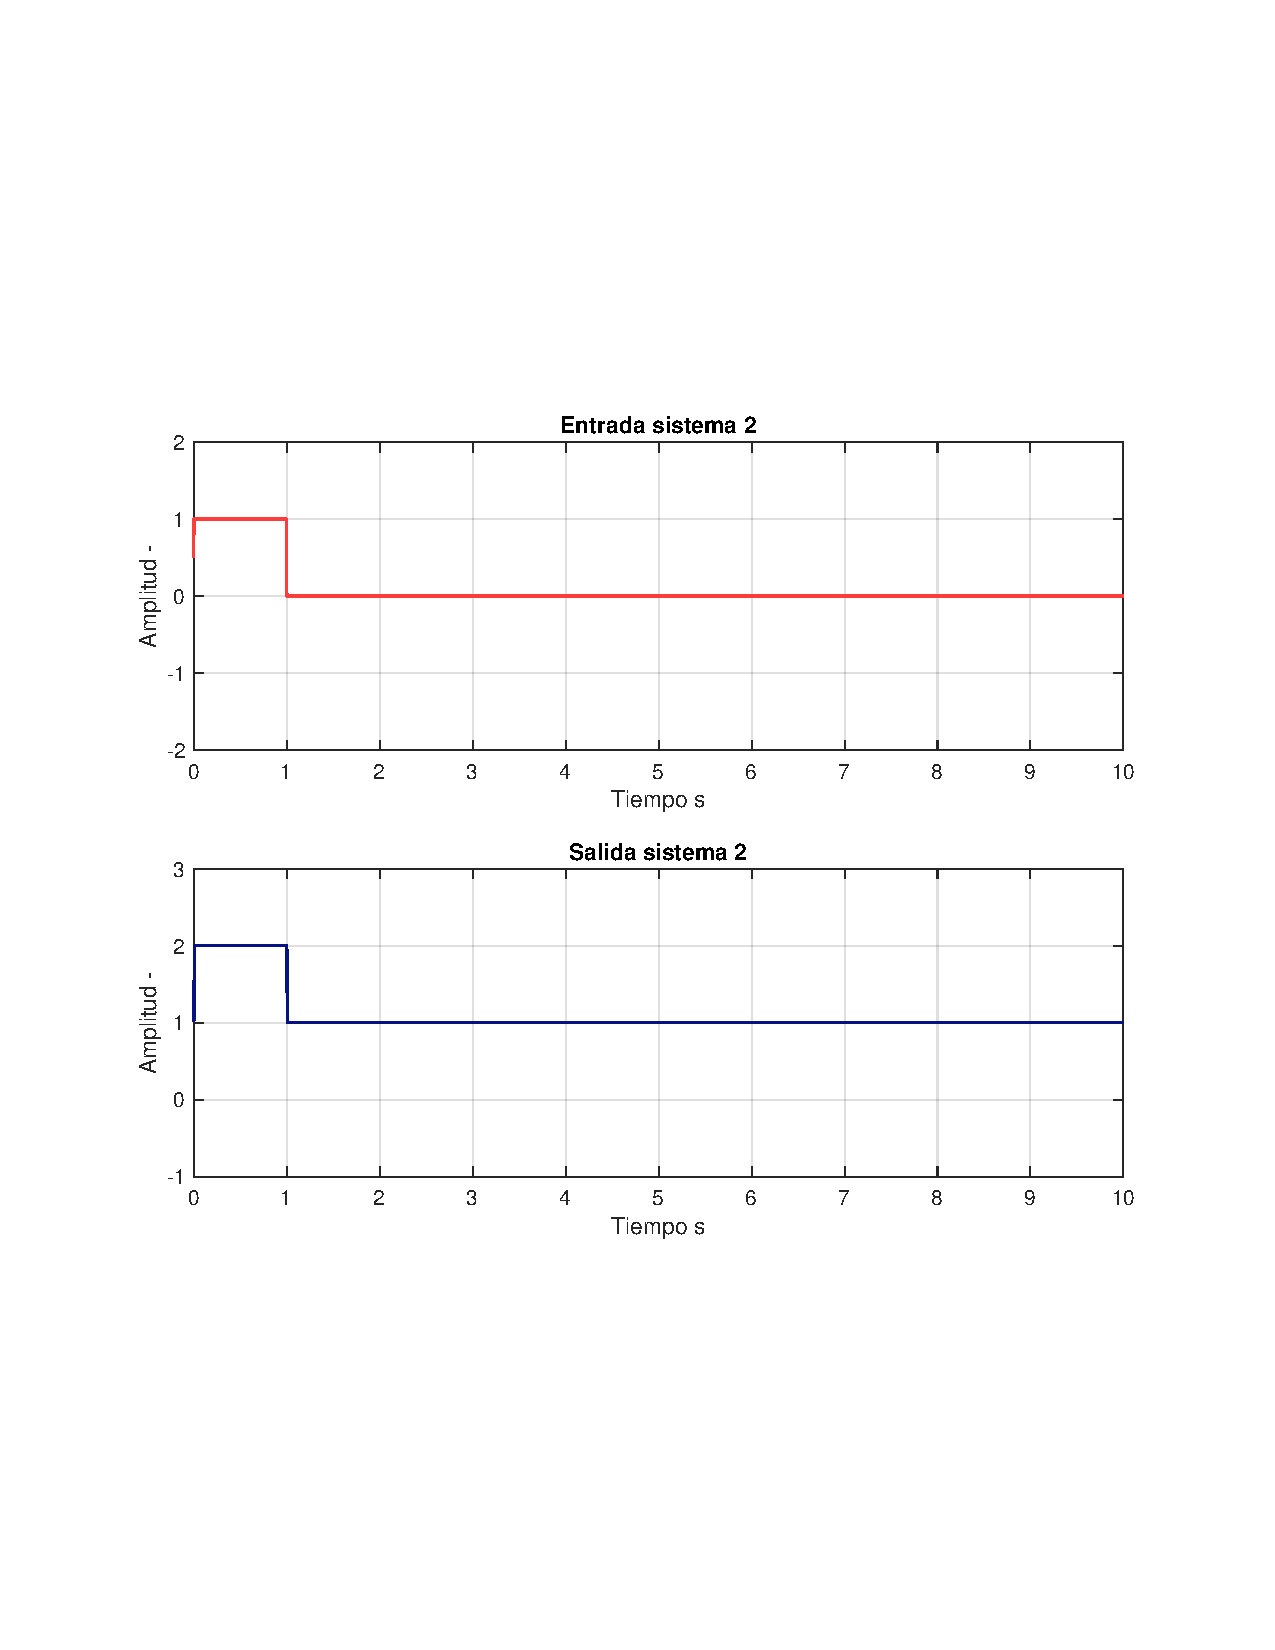
\includegraphics[width=0.6\textwidth,clip, trim = {2cm 7.0cm 2.2cm 7.0cm}]{../imgs/sistema_2_invarianza_temporal_noretardo.pdf}
				\caption{Sistema \#2 Entrada: Pulso cuadrado de duración 1 \textit{s} \textbf{(Arriba)}. Salida del sistema \textbf{(Abajo)}.}
				\label{fig:s_2_time_invariant_test_1}
				\end{figure}
			
				Para un retardo de 5 \textit{s}: 
				\begin{figure}[H]
					\center
					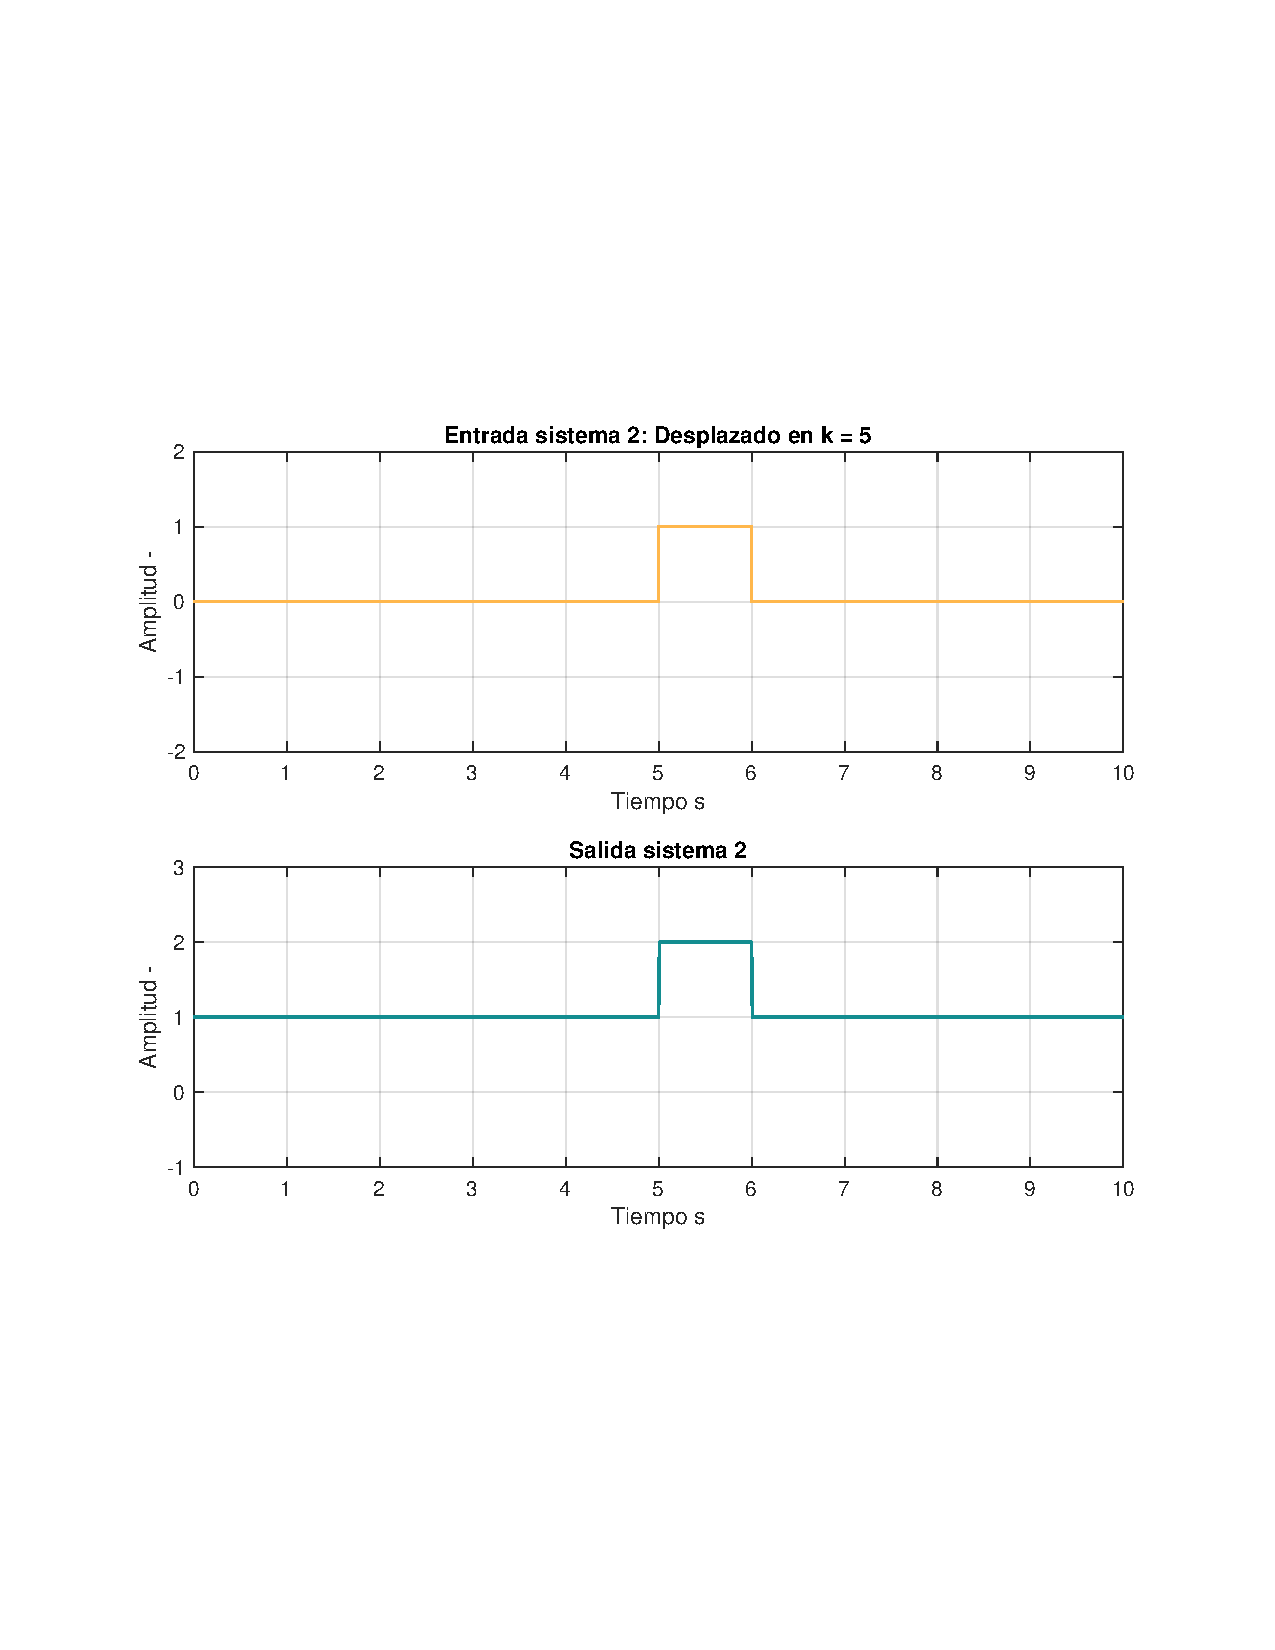
\includegraphics[width=0.6\textwidth,clip, trim = {2cm 7.0cm 2.2cm 7.0cm}]{../imgs/sistema_2_invarianza_temporal_retardo.pdf}
					\caption{Sistema \#2 Entrada: Pulso cuadrado de duración 1 \textit{s}, desplazado en 5 \textit{s} \textbf{(Arriba)}. Salida del sistema \textbf{(Abajo)}.}
					\label{fig:s_2_time_invariant_test_2}
				\end{figure}
			
				Como se ver, al aplicar un retardo sobre la señal de entrada, se obtiene la misma salida sólo que desplazada, cumpliendose la condición descrita en la ecuación \ref{eq:cond_invarianza_temporal}. Por lo que podemos decir que el sistema es \textbf{invariante en el tiempo}. 

\newpage

		\subsubsection{Linealidad}
			Generando las entradas del sistema $u_{1}[n]$ y $u_{2}[n]$:
			\begin{figure}[H]
				\center
				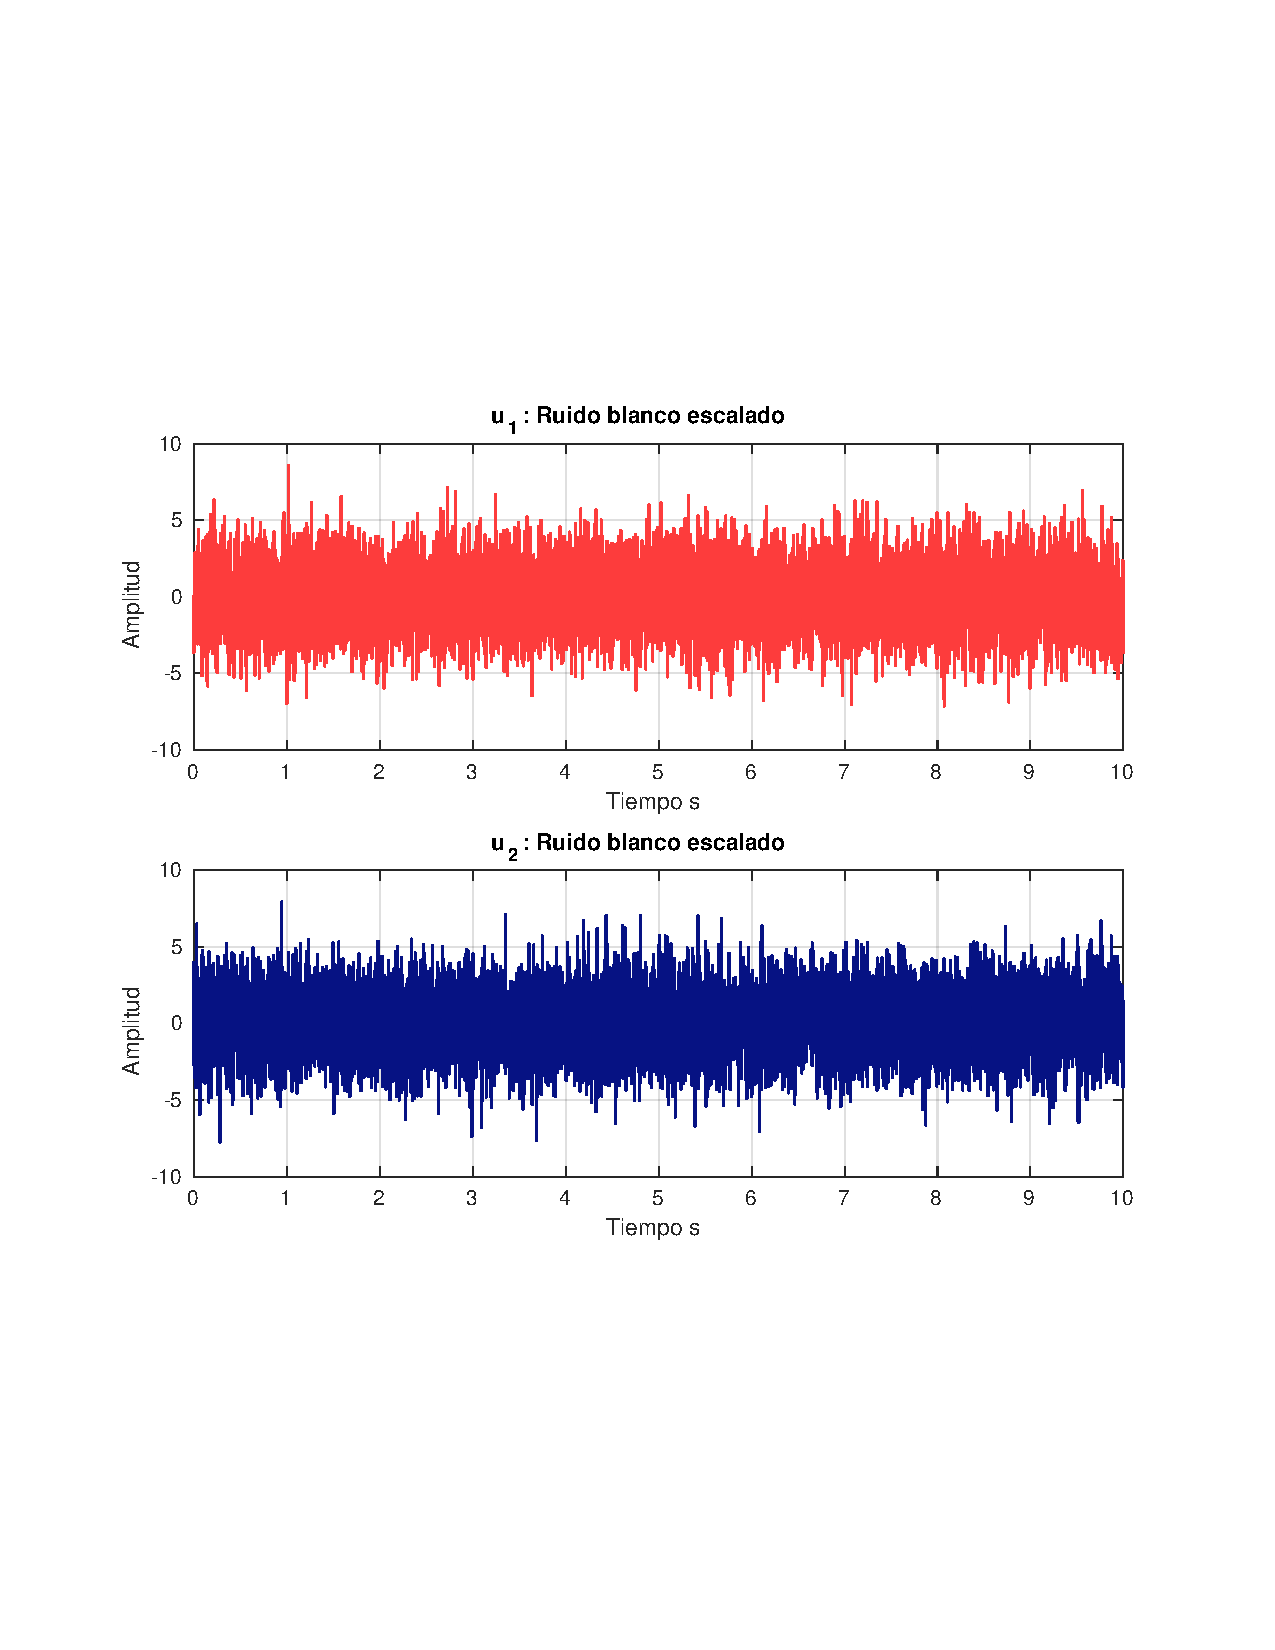
\includegraphics[width=0.6\textwidth,clip, trim = {2cm 7.0cm 2.2cm 7.0cm}]{../imgs/sistema_2_linealidad_entradas.pdf}
				\caption{Entradas del sistema}
				\label{fig:s_2_lineality_inputs}
			\end{figure}
		
			Comprobando las salidas del sistema:
			\begin{figure}[H]
				\center
				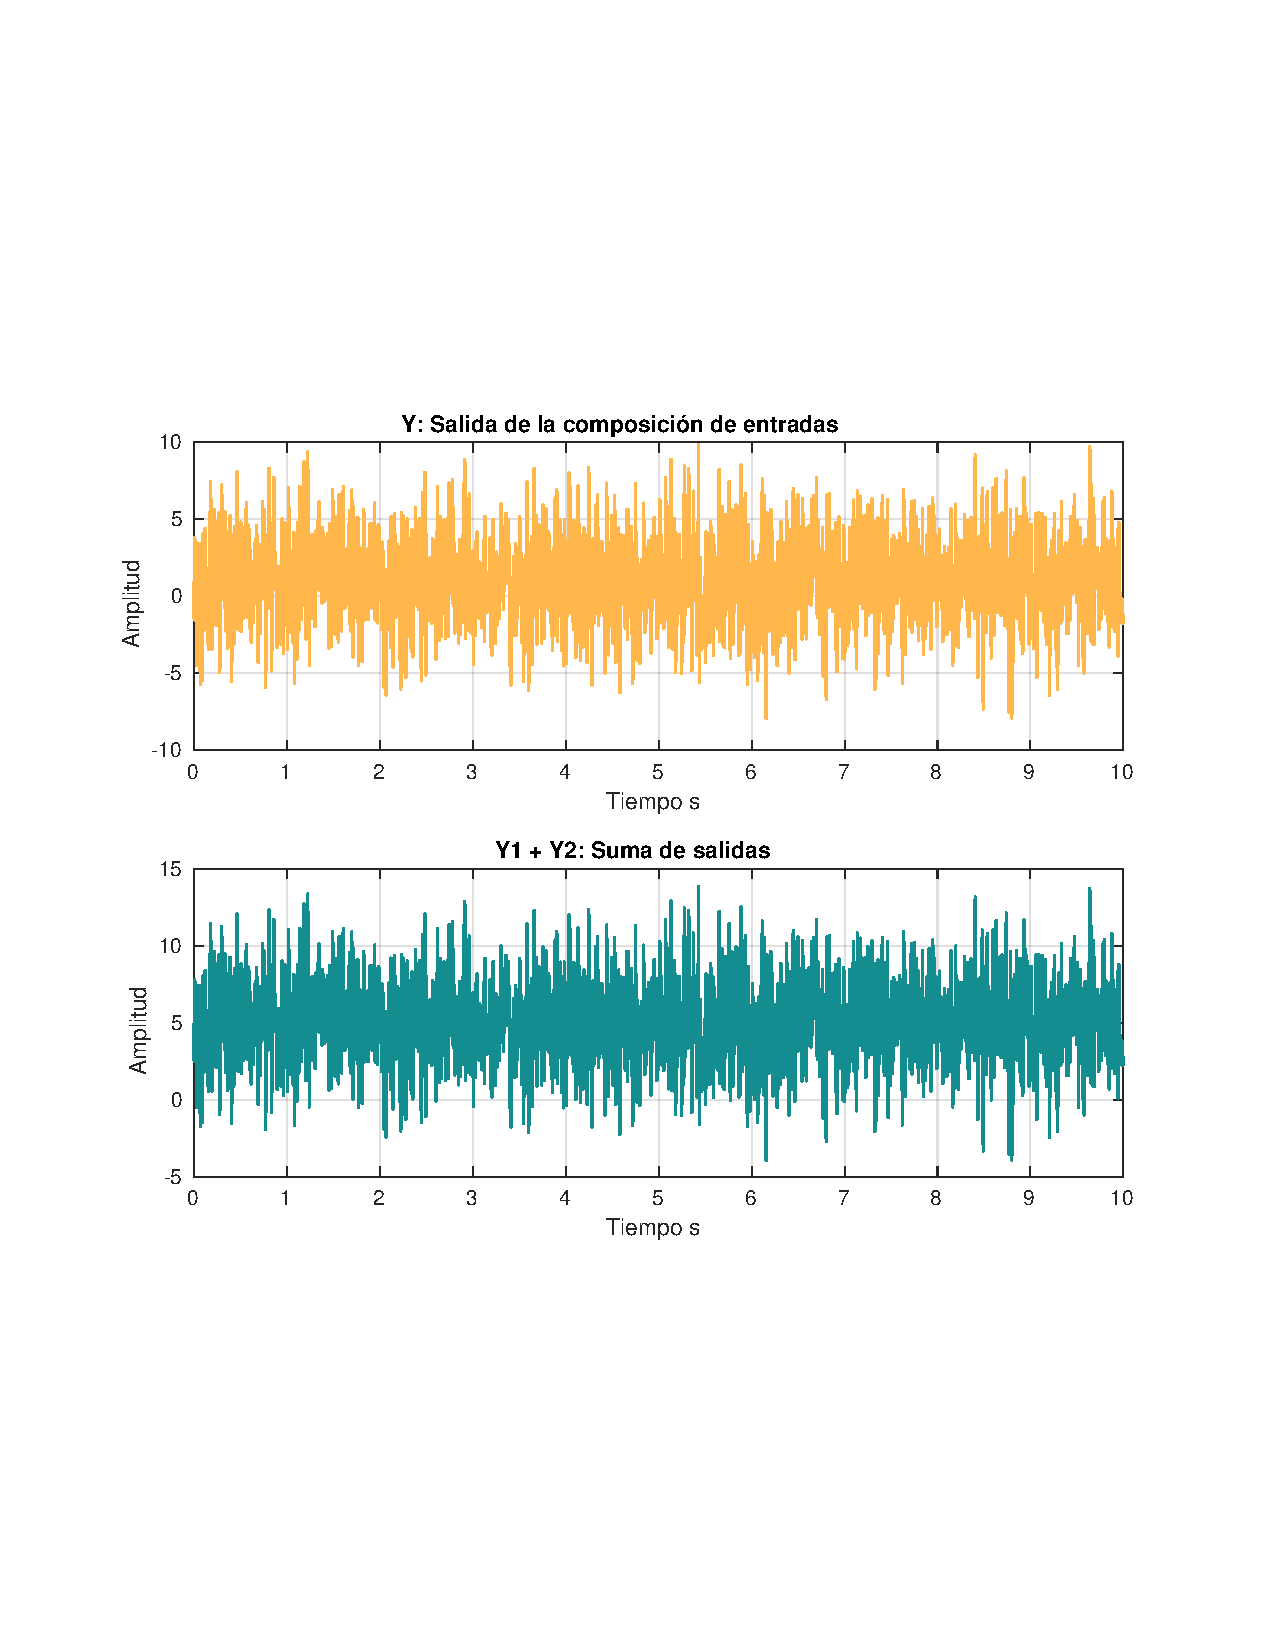
\includegraphics[width=0.6\textwidth,clip, trim = {2cm 7.0cm 2.2cm 7.0cm}]{../imgs/sistema_2_linealidad_salidas.pdf}
				\caption{Salidas del sistema: $Y[n]$ \textbf{(Arriba)}. $Y_{1}[n] + Y_{2}[n]$ \textbf{(Abajo)}.}
				\label{fig:s_2_lineality_outputs}	
			\end{figure}
\newpage
			Realizando la comparación de salidas:
			\begin{figure}[H]
				\center
				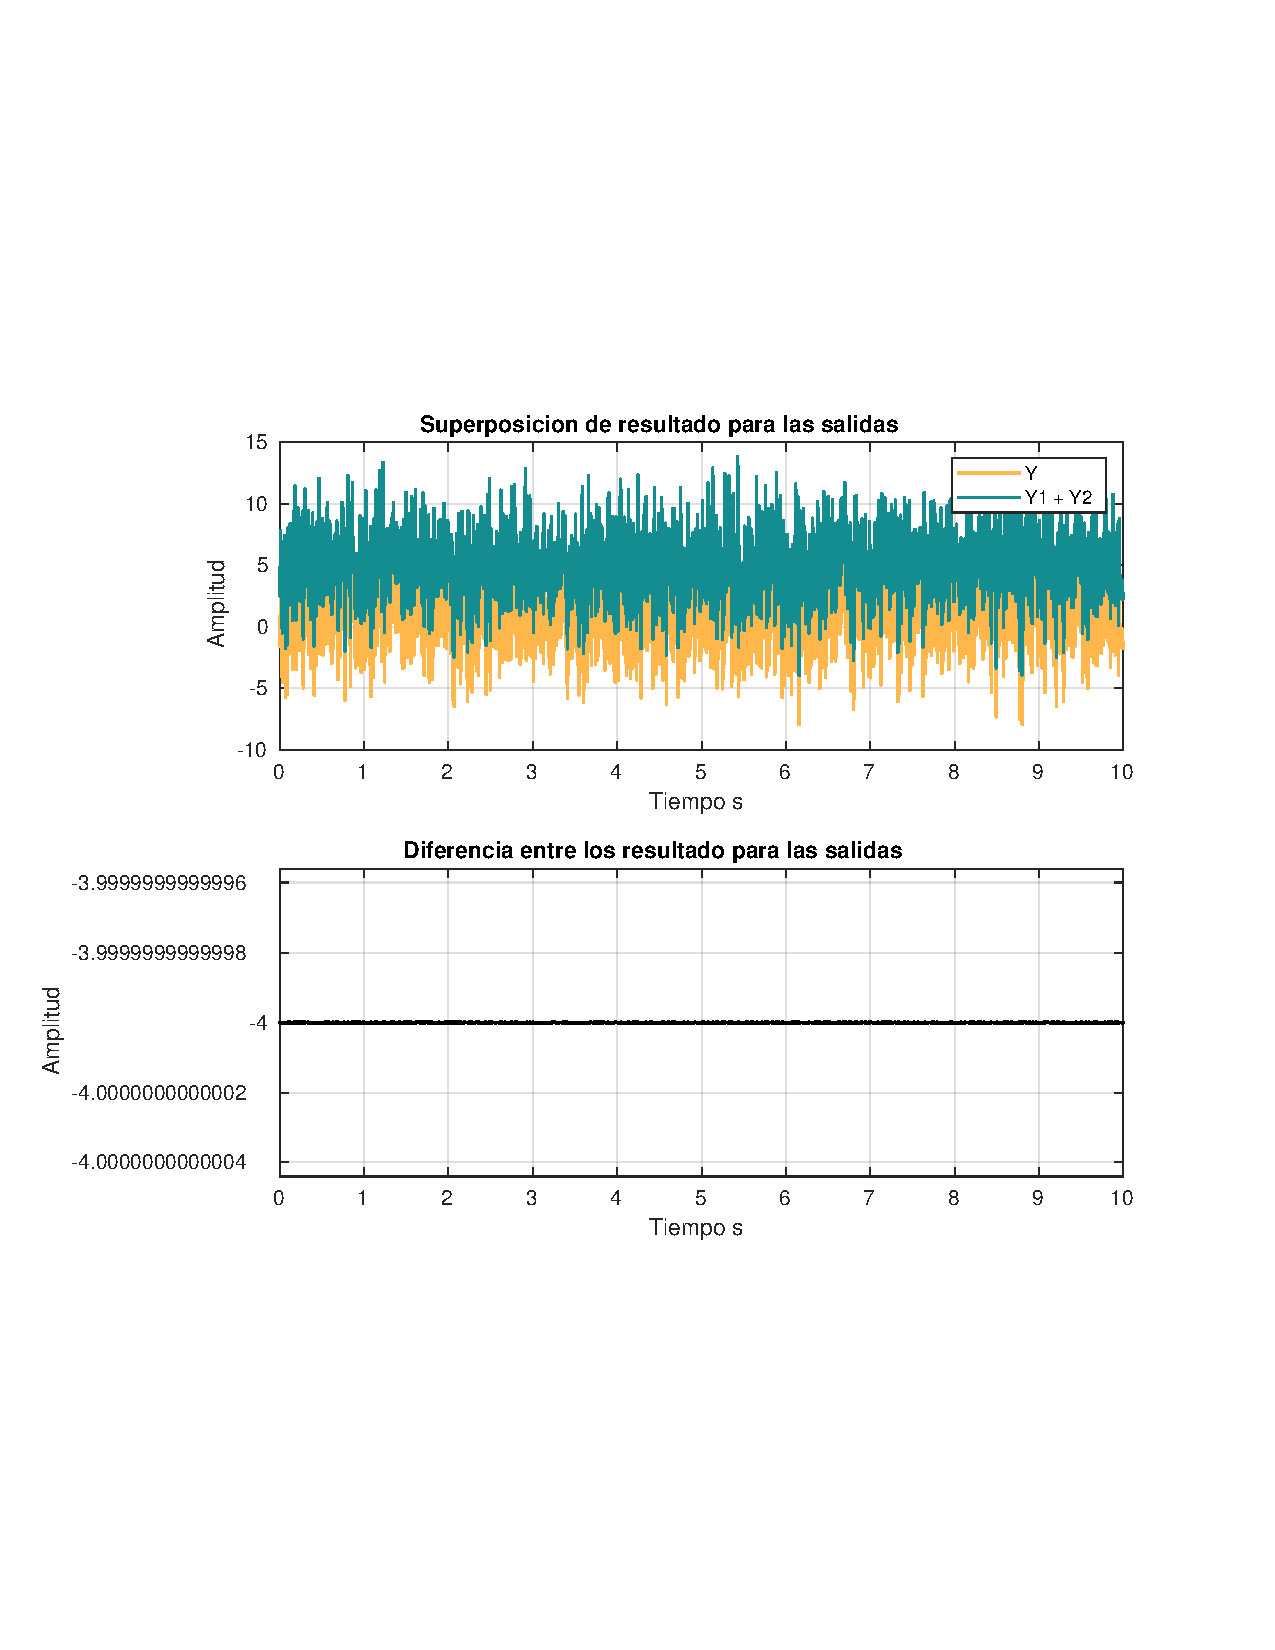
\includegraphics[width=0.6\textwidth,clip, trim = {2cm 7.0cm 2.2cm 7.0cm}]{../imgs/sistema_2_linealidad_superpuestas.pdf}
				\caption{Superposición de las señales de salida \textbf{(Arriba)}. Representación de la resta punto a punto de las señales. \textbf{(Abajo)}.}
				\label{fig:s_2_lineality_superposition}
			\end{figure}
		
			Como se puede ver, en la figura \ref{fig:s_2_lineality_outputs}, ambas salidas son muy similares, sin embargo, la salida que corresponde al resultado del lado derecho de la ecuación \ref{eq:cond_linealidad}, parece faltarle un nivel continuo, lo que queda en evidencia al calcular la diferencia de ambas entradas, figura \ref{fig:s_2_lineality_superposition}. Por lo que podemos concluir que el sistema \textbf{no es lineal}.
		
		\subsubsection{Estabilidad BIBO}
			Aplicandole al sistema un delta de Kronecker:
		
			\begin{figure}[H]
				\center
				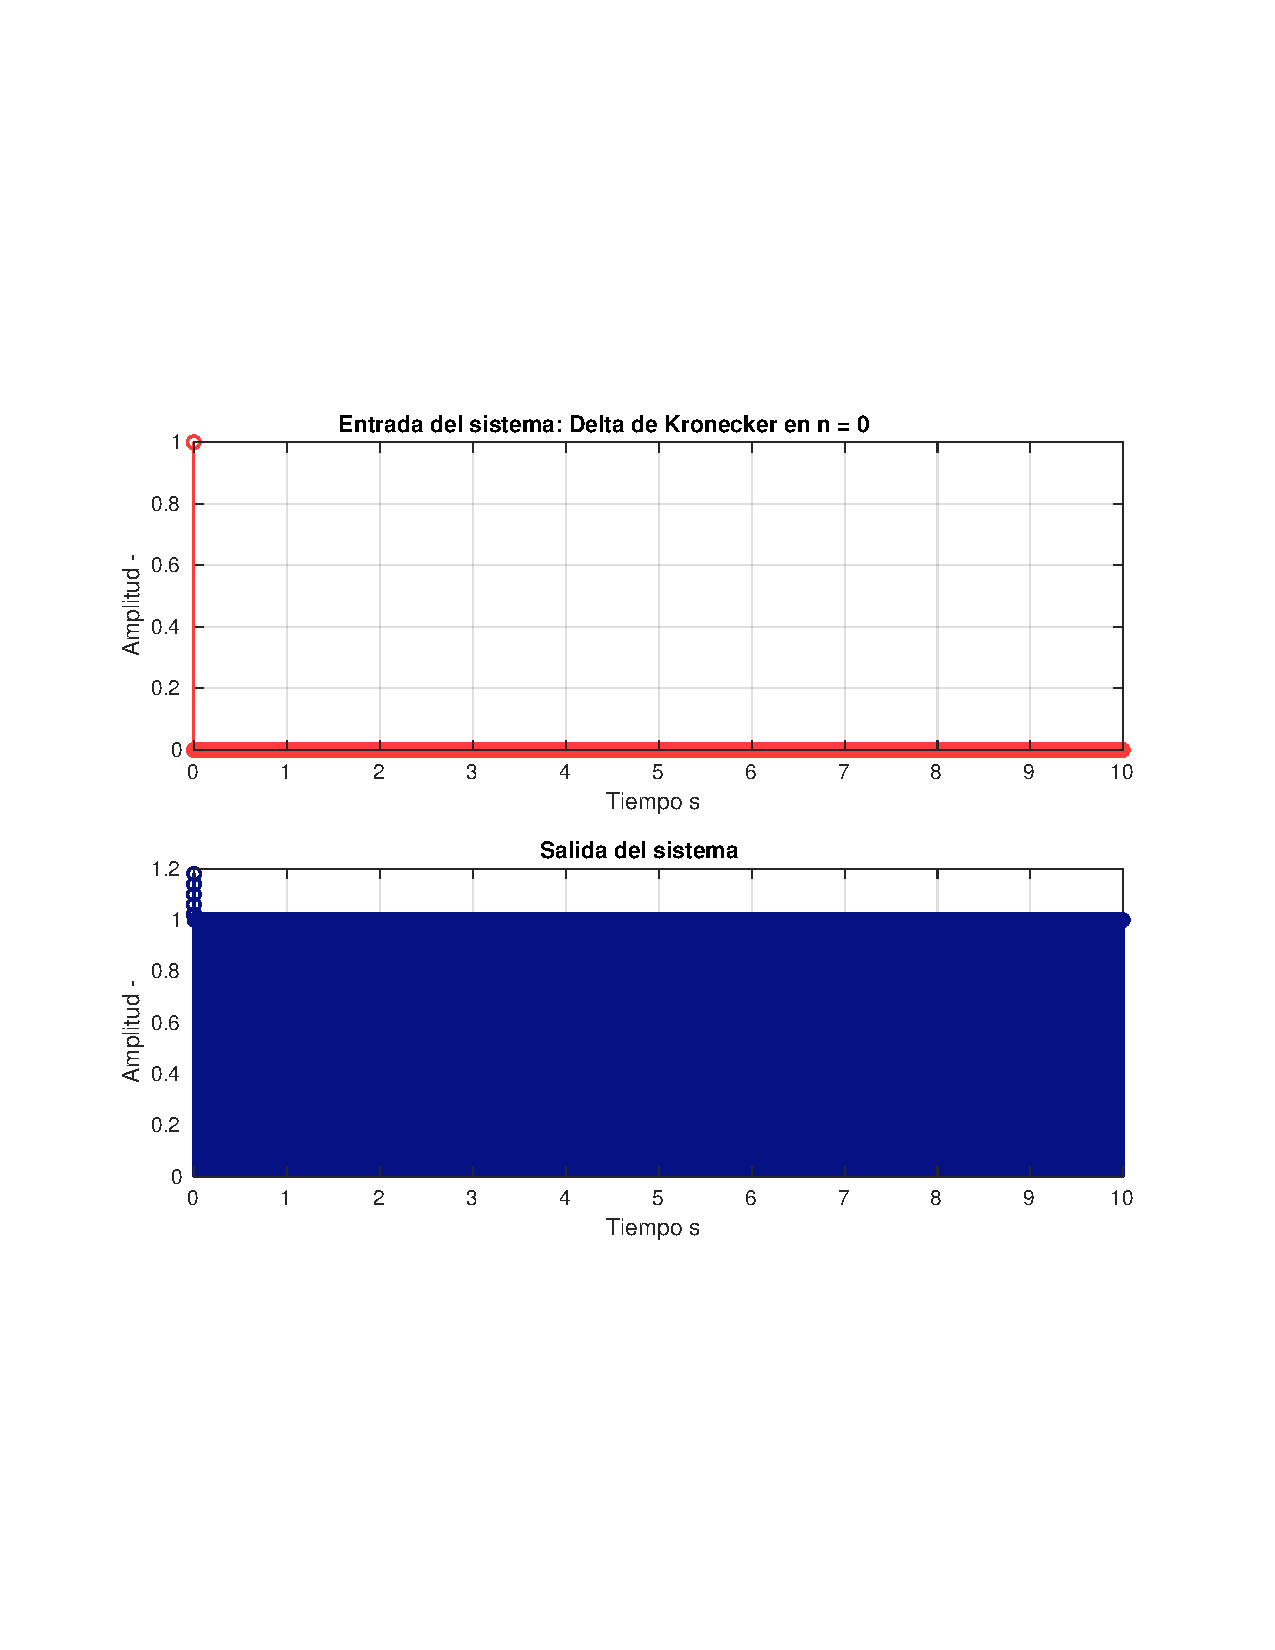
\includegraphics[width=0.6\textwidth,clip, trim = {2cm 7.0cm 2.2cm 7.0cm}]{../imgs/sistema_2_bibo_n_0.pdf}
				\caption{Sistema \#2, para una entrada de un delta de Kronecker \textbf{(Arriba)}, para la cual se tiene la siguiente respuesta \textbf{(Abajo)}.}
				\label{fig:s_2_bibo_n_0}
			\end{figure}
		
			Podemos ver que la salida del sistema, se comporta como la entrada más una constante, algo que ya se había notado durante la comprobación de linealidad del sistema. A partir del resultado, para esta señal, podemos decir que para un delta, el sistema es estable. Procediendo a probar con un escalón unitario:
		
			\begin{figure}[H]
				\center
				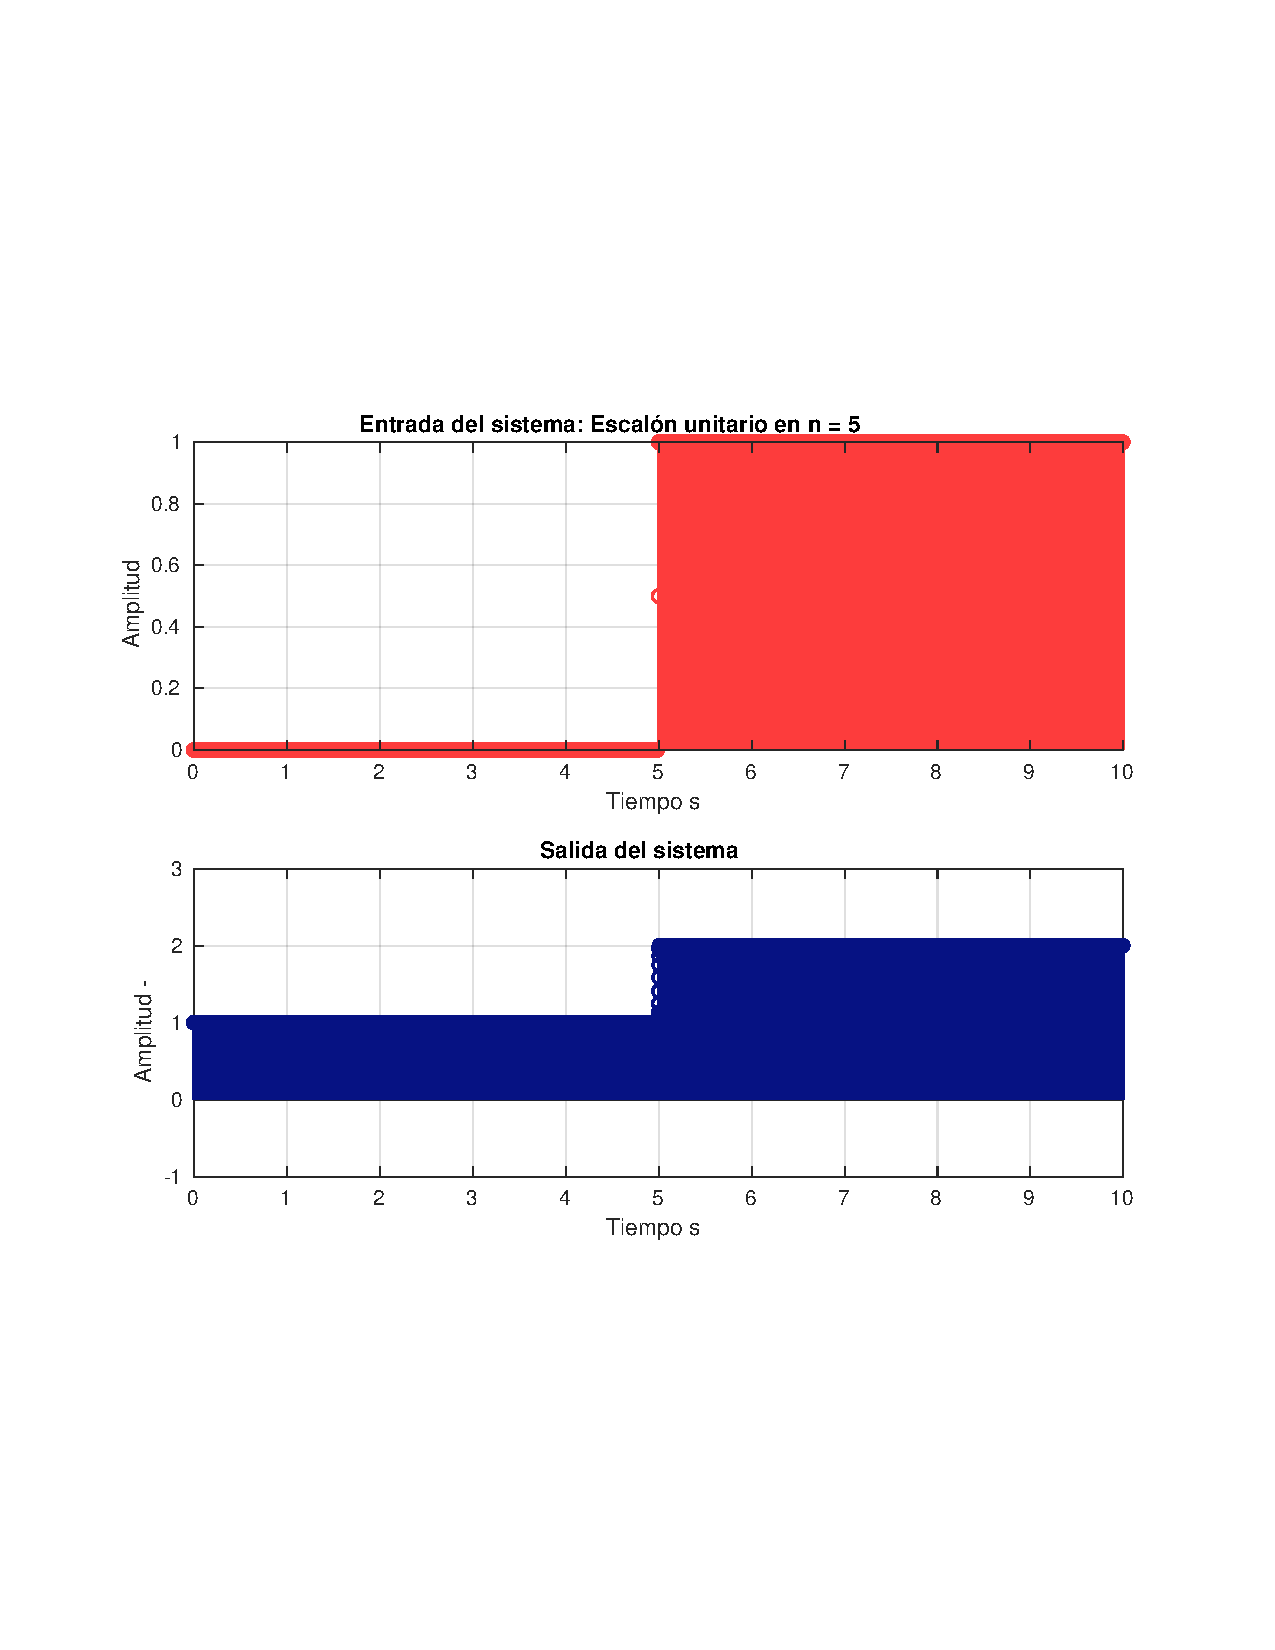
\includegraphics[width=0.6\textwidth,clip, trim = {2cm 7.0cm 2.2cm 7.0cm}]{../imgs/sistema_2_bibo_heaviside_n_5.pdf}
				\caption{Sistema \#2, para una entrada de escalón unitario, activado en n = 5 \textbf{(Arriba}}, para el cual se tiene la siguiente respuesta \textbf{(Abajo)}. 
				\label{fig:s_2_bibo_heaviside_n_5}
			\end{figure}
		
			Para esta salida, también se tiene que el sistema responde sumándole a la entrada una constante. Nuevamente, la respuesta para esta entrada es acotada. Siguiendo con la última señal de prueba, una señal triangular de amplitud 1 y frecuencia 1 \textit{Hz}: 
			\begin{figure}[H]
				\center
				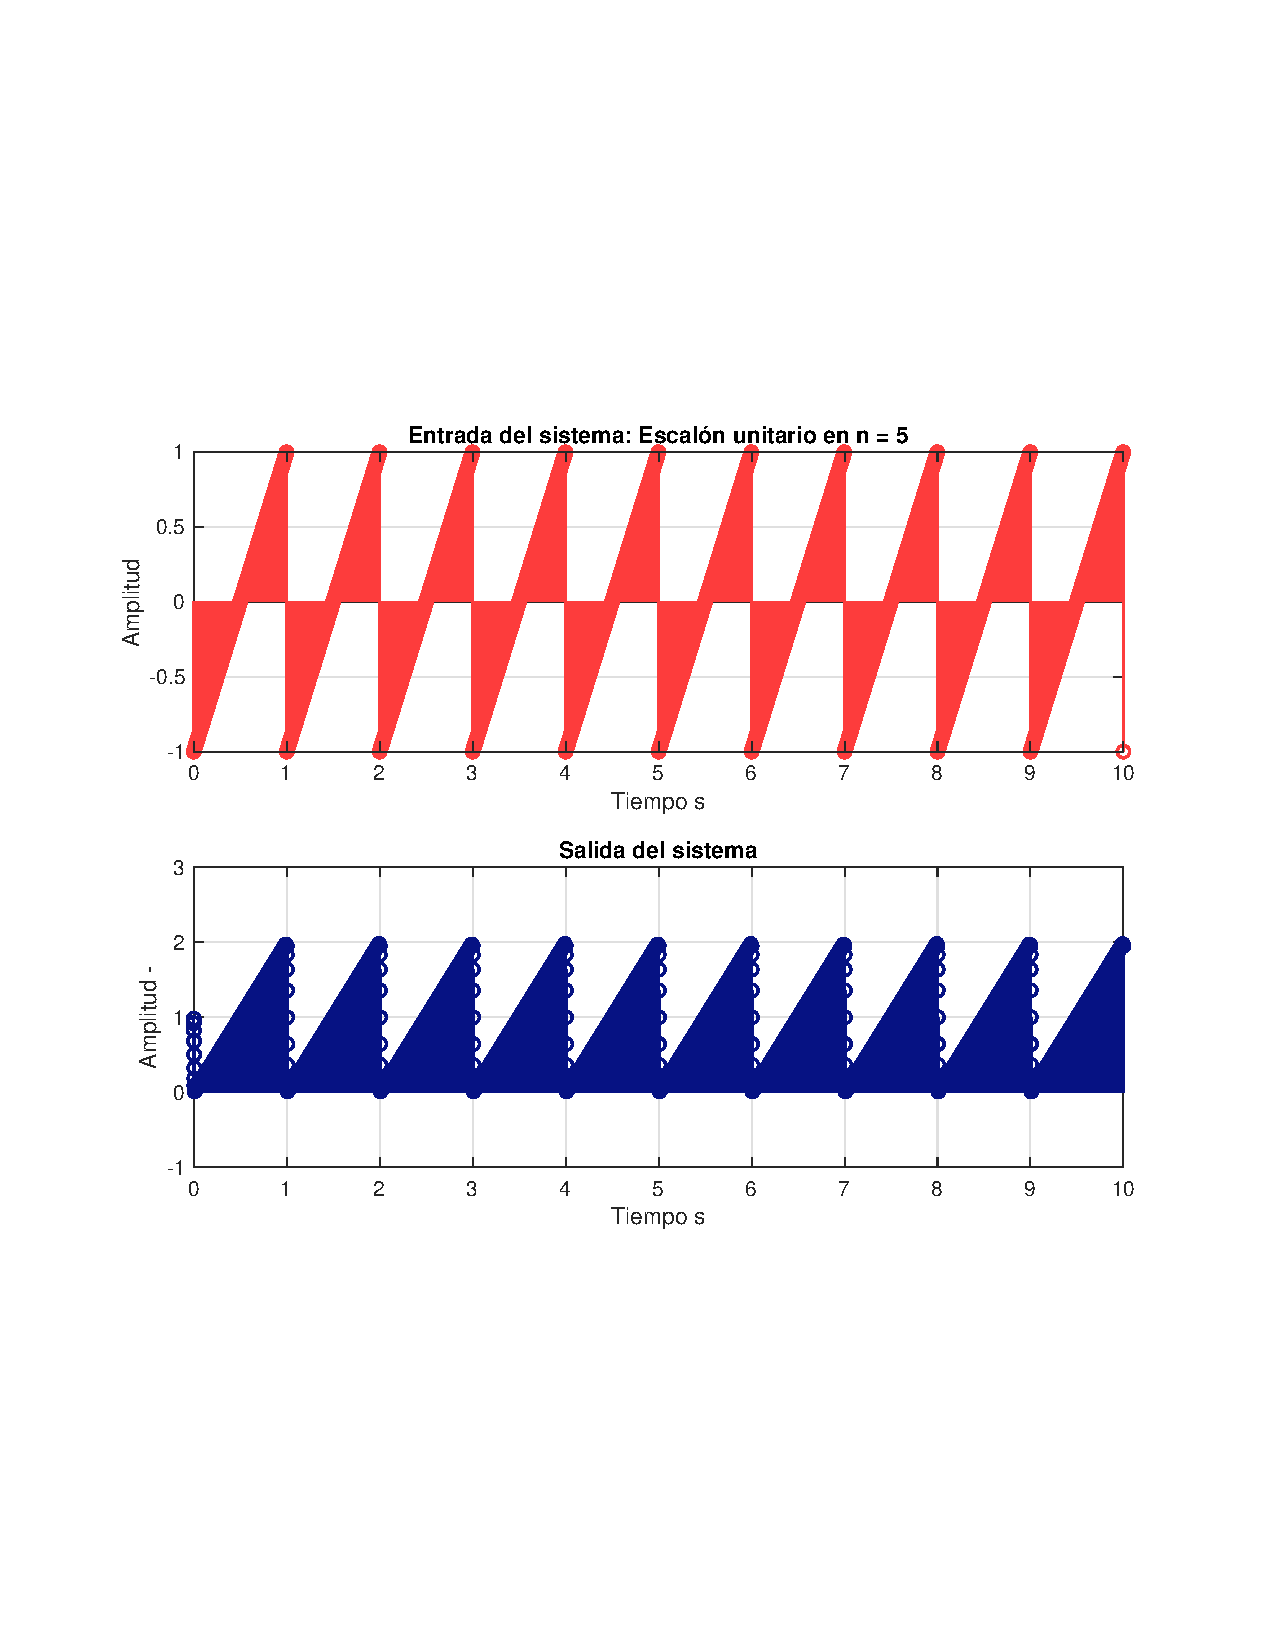
\includegraphics[width=0.6\textwidth,clip, trim = {2cm 7.0cm 2.2cm 7.0cm}]{../imgs/sistema_2_bibo_sawtooth.pdf}
				\caption{Sistema \#2, para una entrada de señal triangular \textbf{(Arriba)}, se tiene la siguiente salida \textbf{(Abajo)}.}
				\label{fig:s_2_bibo_sawtooth}
			\end{figure}
		
			Nuevamente, el resultado obtenido es idéntico, a la señal de entrada se le suma una constante, por lo que nuevamente es acotada. Tomando en consideración estos resultados, \textbf{se puede especular que el sistema es BIBO estable}.

\newpage

	\subsection{Sistema \#3}
		\subsubsection{Invariancia temporal}
			Aplicando la señal de prueba en el sistema, con retardo igual a cero: 
			\begin{figure}[H]
				\center
				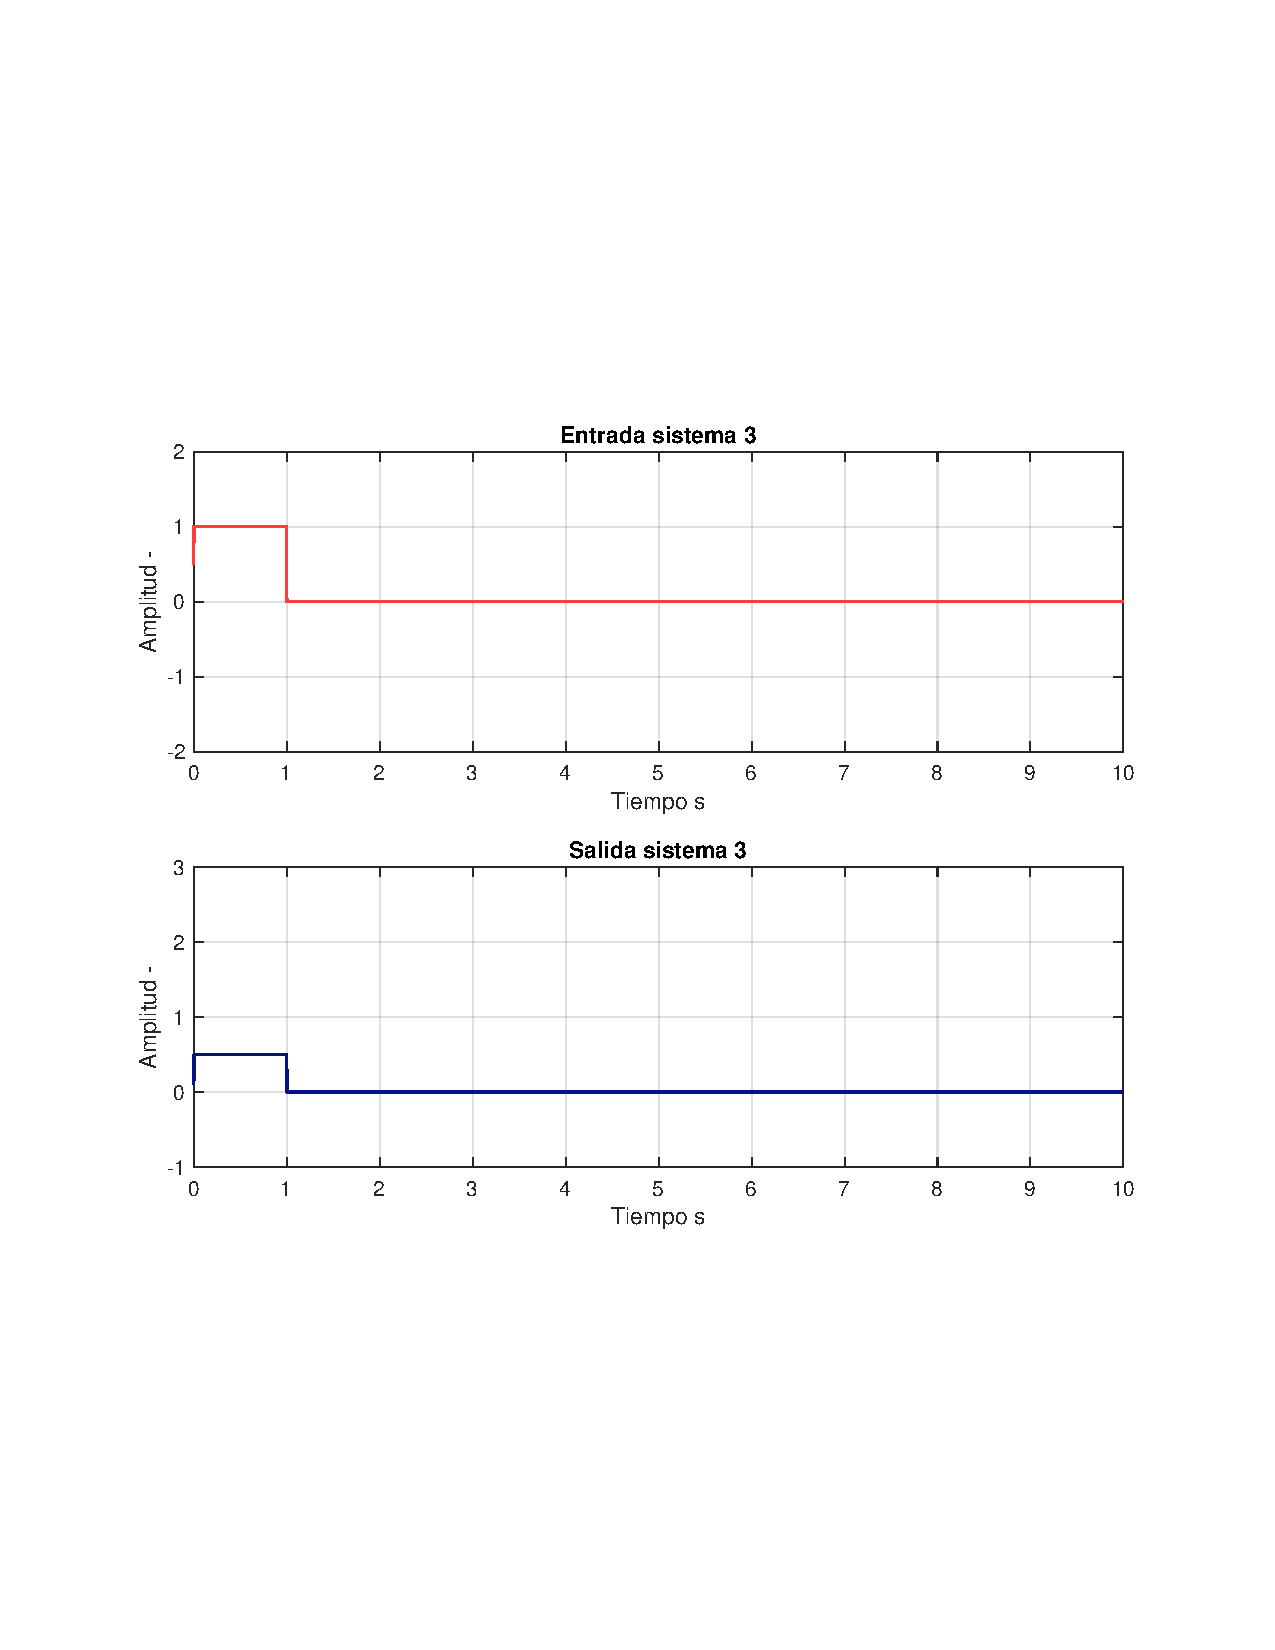
\includegraphics[width=0.6\textwidth,clip, trim = {2cm 7.0cm 2.2cm 7.0cm}]{../imgs/sistema_3_invarianza_temporal_noretardo.pdf}
				\caption{Sistema \#3 Entrada: Pulso cuadrado de duracion 1 \textit{s} \textbf{(Arriba)}. Salida del sistema \textbf{(Abajo)}.}
				\label{fig:s_3_time_invariant_test_1}
			\end{figure}
			Para un retardo de 5 s:
			\begin{figure}[H]
				\center
				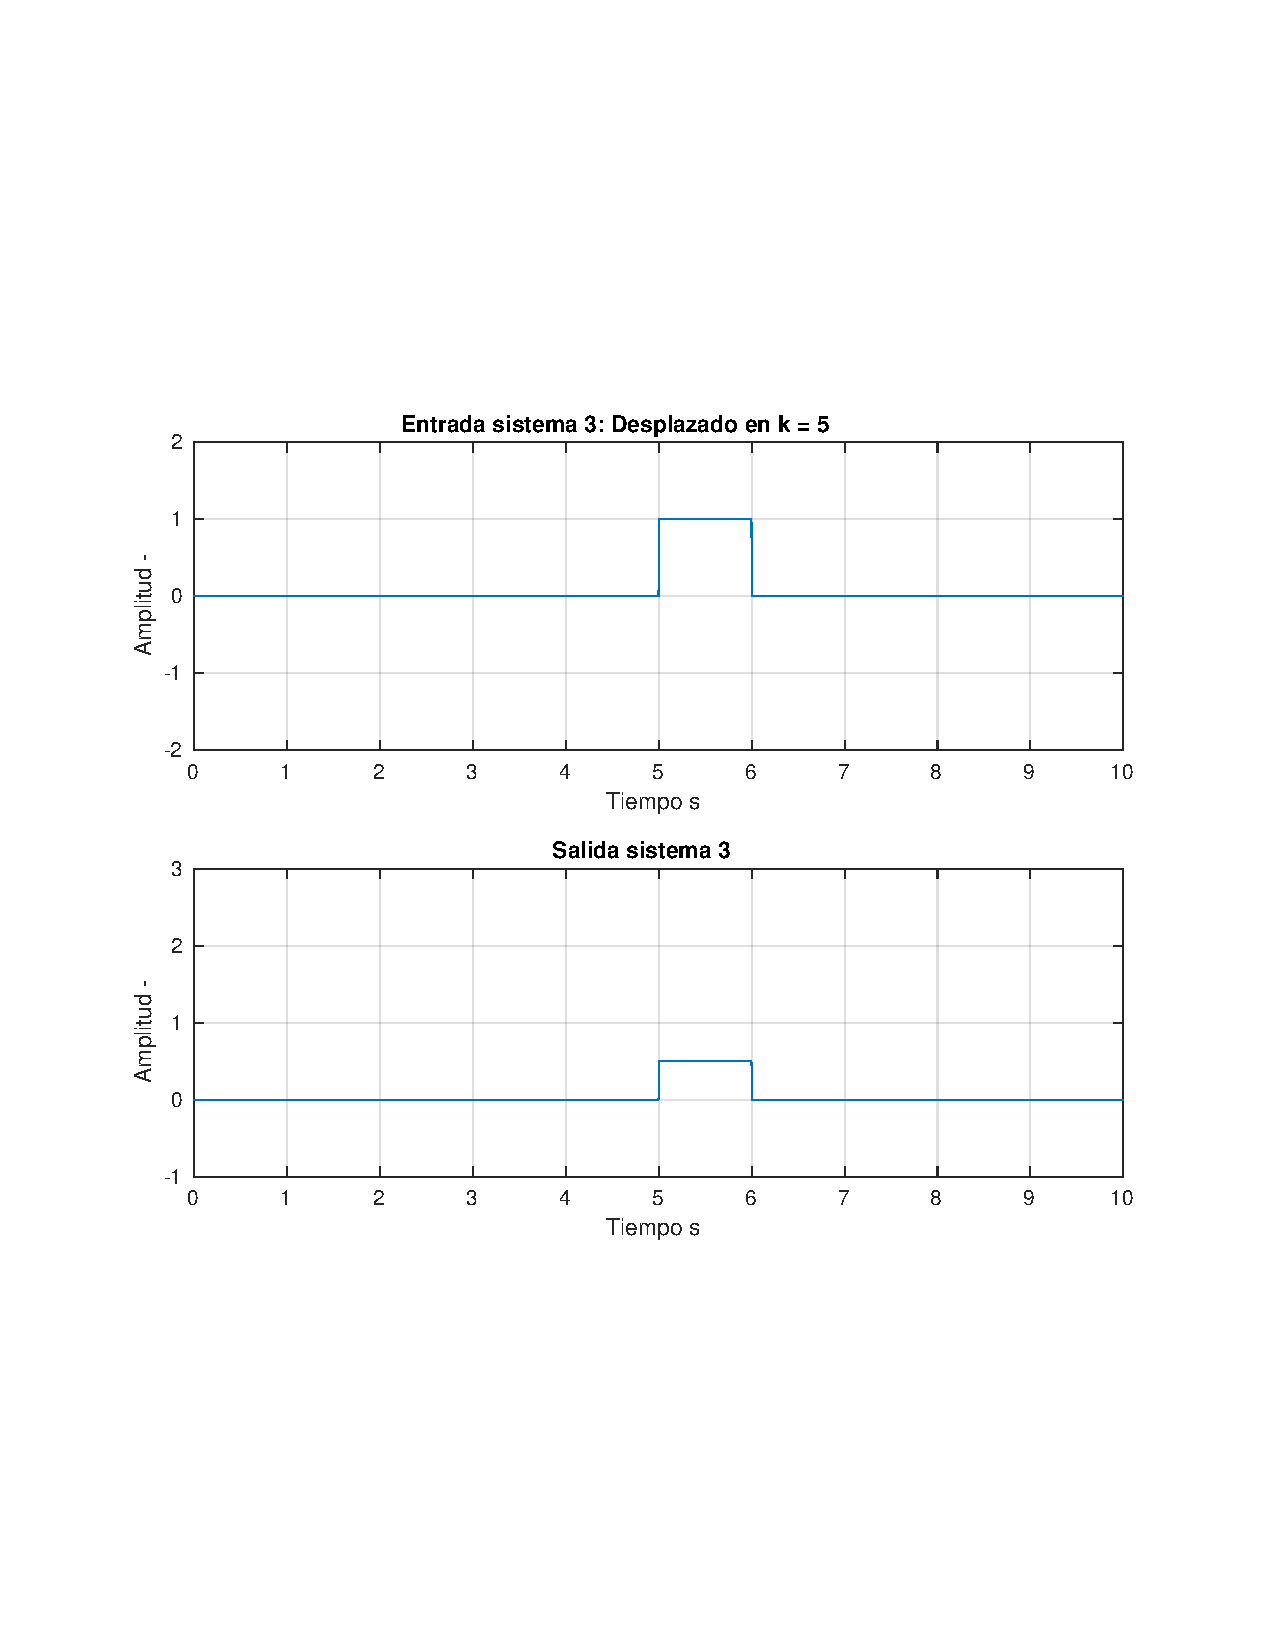
\includegraphics[width=0.6\textwidth,clip, trim = {2cm 7.0cm 2.2cm 7.0cm}]{../imgs/sistema_3_invarianza_temporal_retardo.pdf}
				\caption{Sistema \#3 Entrada: Pulso cuadrado de duracion 1 \textit{s}, desplazado en 5 \textit{s} \textbf{(Arriba)}. Salida del sistema \textbf{(Abajo)}.}
				\label{fig:s_3_time_invariant_test_2}
			\end{figure}
			
			Se obtiene la misma salida, simplemente desplazada, cumpliendo la condición de la ecuación \ref{eq:cond_invarianza_temporal}. Se puede decir que el sistema es \textbf{invariante en el tiempo}.

\newpage

		\subsubsection{Linealidad}
			Generando las entradas del sistema $u_{1}[n]$ y $u_{2}[n]$:
			\begin{figure}[H]
				\center
				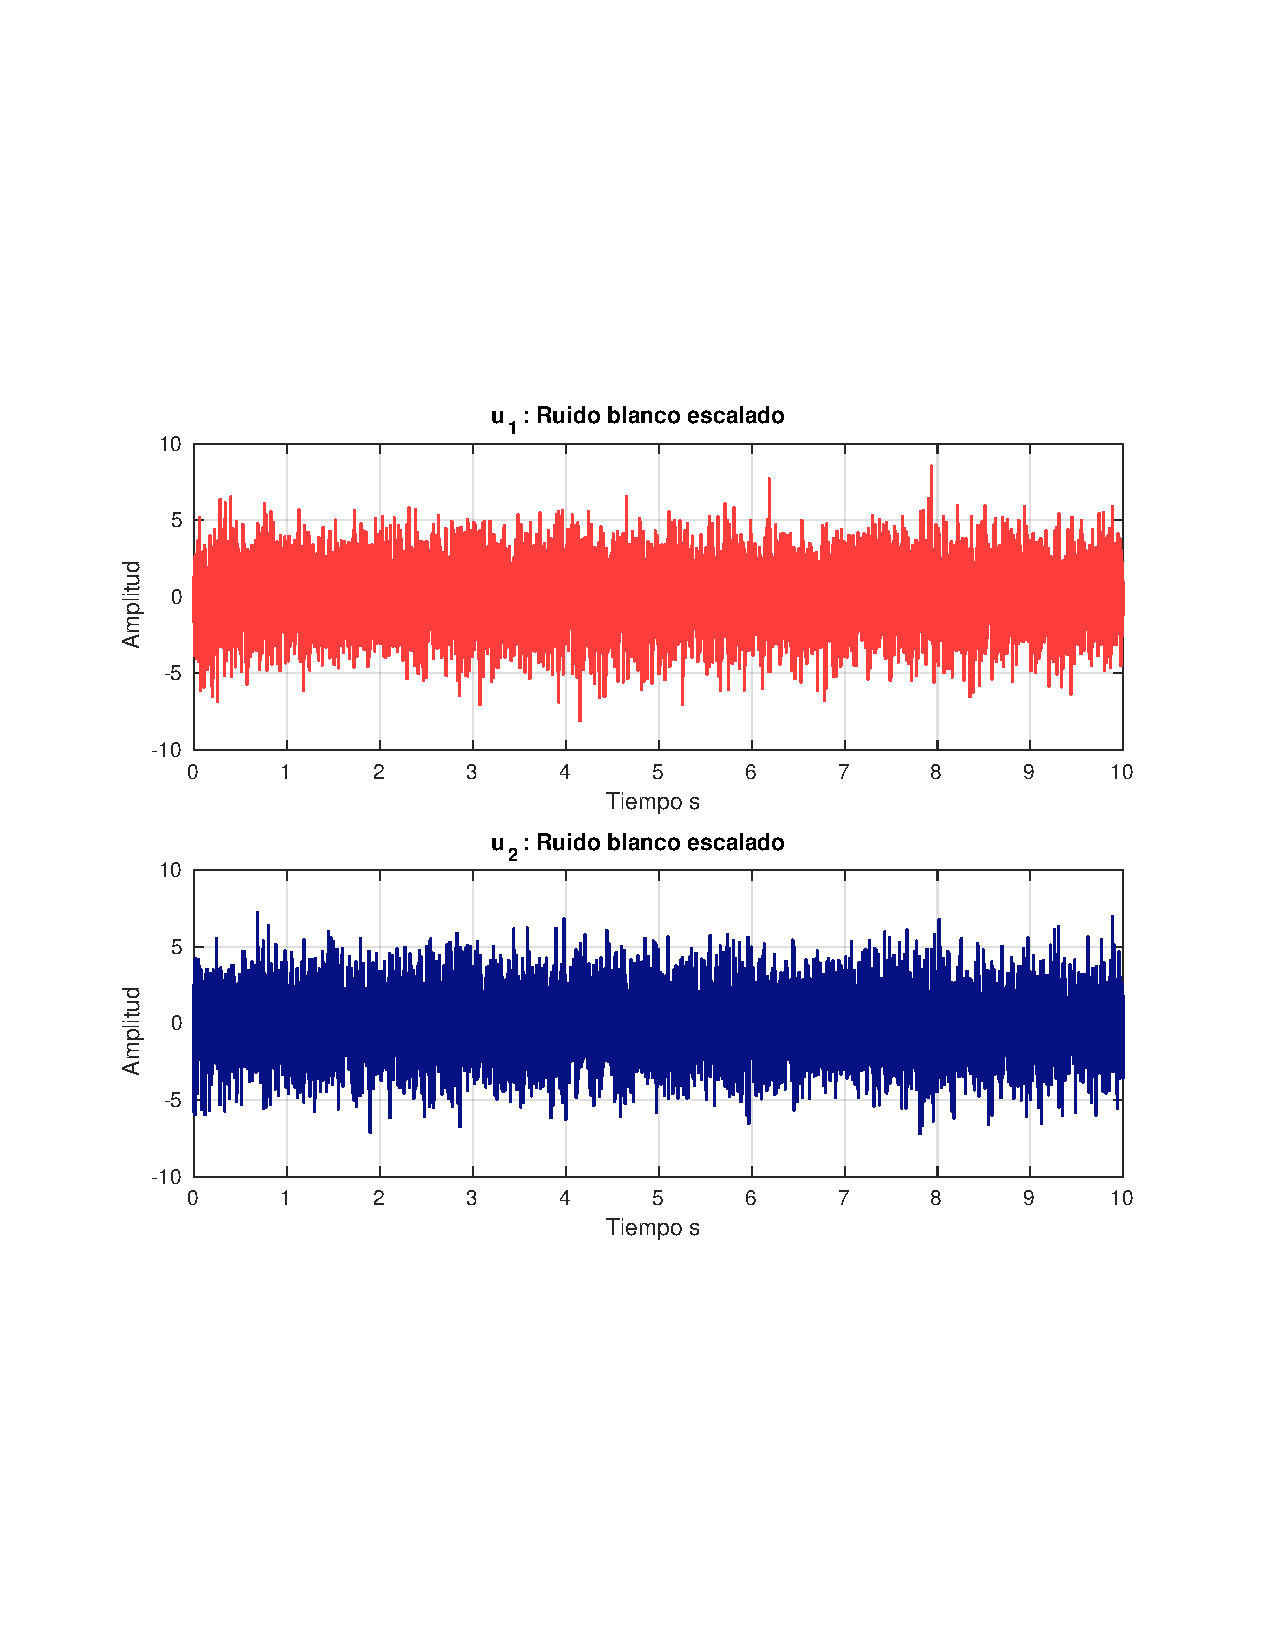
\includegraphics[width=0.6\textwidth,clip, trim = {2cm 7.0cm 2.2cm 7.0cm}]{../imgs/sistema_3_linealidad_entradas.pdf}
				\caption{Entradas del sistema}
				\label{fig:s_3_lineality_inputs}
			\end{figure}
			Comprobando las salidas del sistema:
			\begin{figure}[H]
				\center
				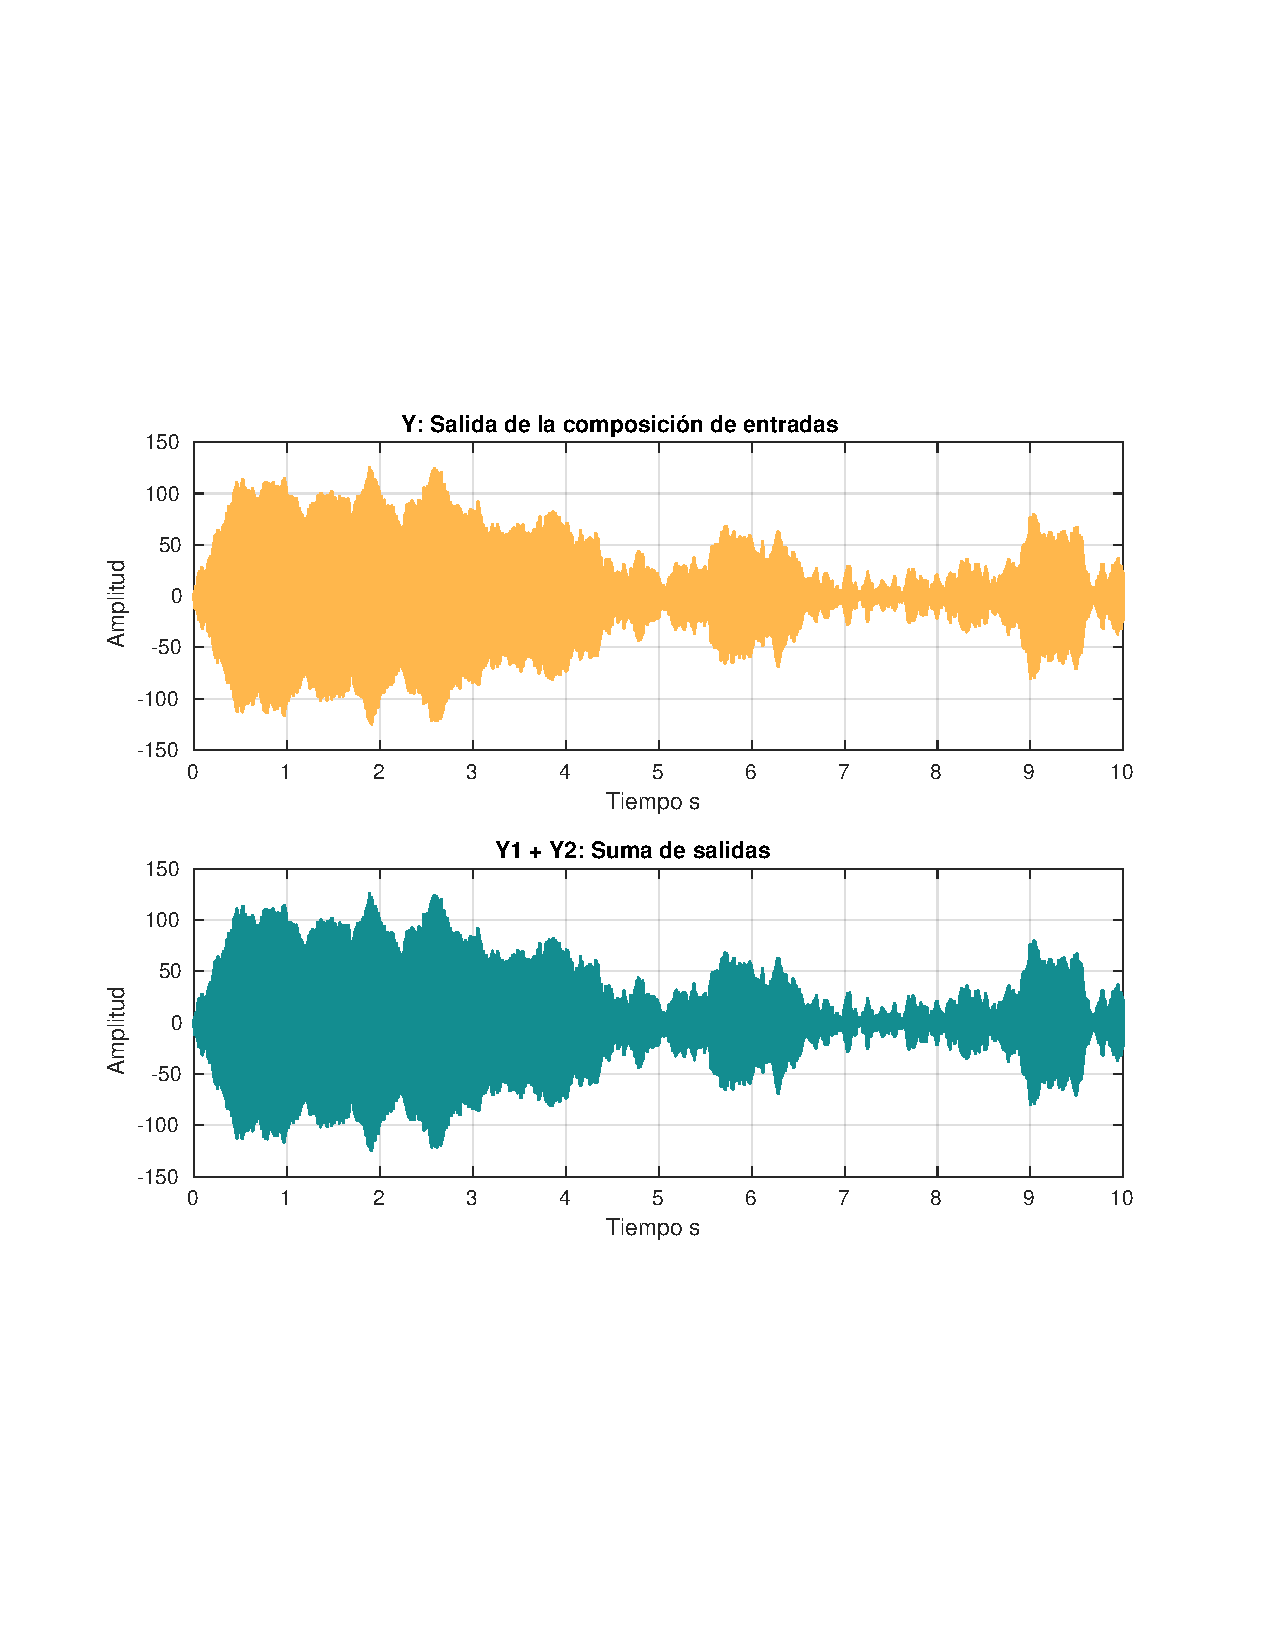
\includegraphics[width=0.6\textwidth,clip, trim = {2cm 7.0cm 2.2cm 7.0cm}]{../imgs/sistema_3_linealidad_salidas.pdf}
				\caption{Salidas del sistema: $Y[n]$ \textbf{(Arriba)}. $Y_{1}[n] + Y_{2}[n]$ \textbf{(Abajo)}.}
				\label{fig:s_3_lineality_outputs}	
			\end{figure}

\newpage			

			Realizando la comparación de salidas:
			\begin{figure}[H]
				\center
				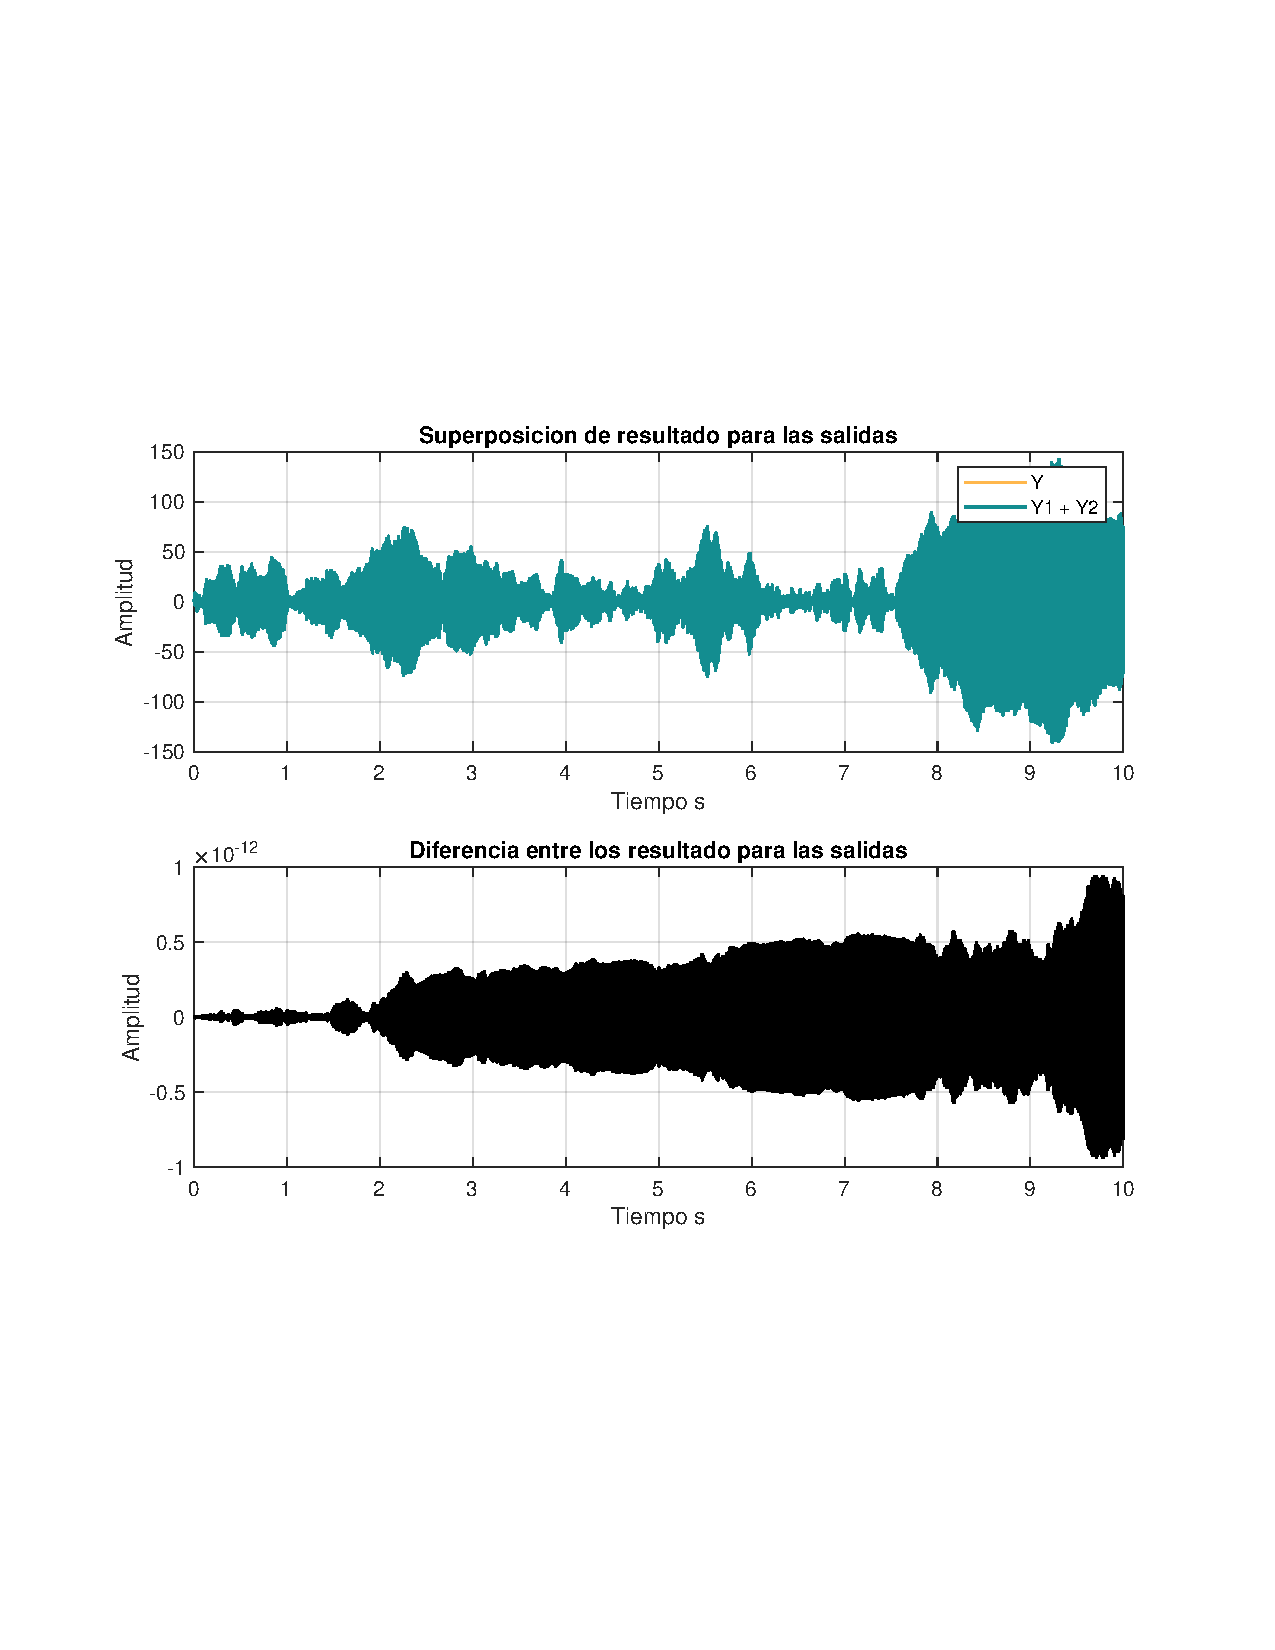
\includegraphics[width=0.6\textwidth,clip, trim = {2cm 7.0cm 2.2cm 7.0cm}]{../imgs/sistema_3_linealidad_superpuestas.pdf}
				\caption{Superposición de las señales de salida \textbf{(Arriba)}. Representación de la resta punto a punto de las señales. \textbf{(Abajo)}.}
				\label{fig:s_3_lineality_superposition}
			\end{figure}
			
			Dado el resultado obtenido en la figura \ref{fig:s_3_lineality_outputs}, ambas señales son identicas, hecho que es comprobado en la figura \ref{fig:s_3_lineality_superposition}, donde se puede comprobar que la diferencia de ambas señales es del orden de $10^{-12}$. Por lo que se puede decir que el sistema cumple \textbf{linealidad}.
			
		\subsubsection{Estabilidad BIBO}
			Aplicandole al sistema un delta de Kronecker:
		
			\begin{figure}[H]
				\center
				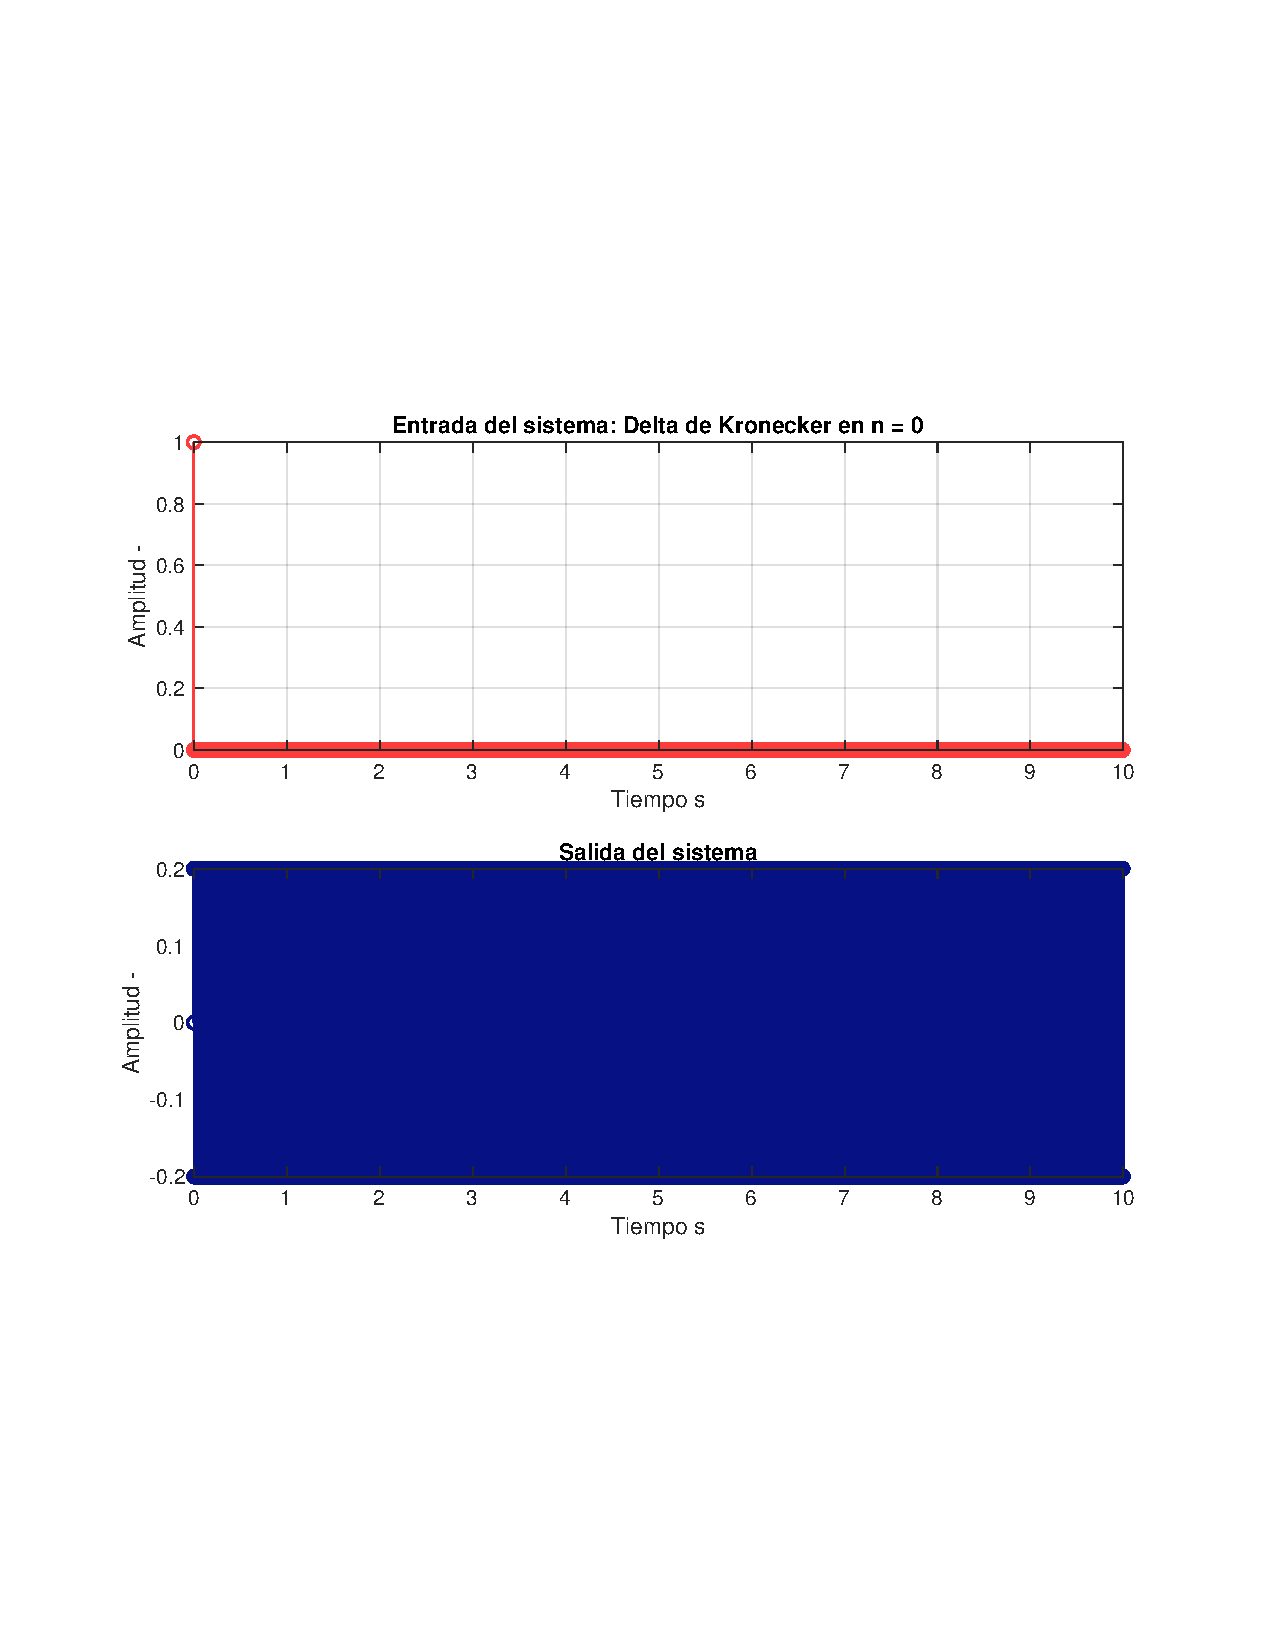
\includegraphics[width=0.6\textwidth,clip, trim = {2cm 7.0cm 2.2cm 7.0cm}]{../imgs/sistema_3_bibo_n_0.pdf}
				\caption{Sistema \#3, para una entrada de un delta de Kronecker \textbf{(Arriba)}, para la cual se tiene la siguiente respuesta \textbf{(Abajo)}.}
				\label{fig:s_3_bibo_n_0}
			\end{figure}
		
			A la salida del sistema, se obtiene una señal que se asemeja a un escalón unitario, el cual es acotado. A partir del resultado, para esta señal, podemos decir que para un delta, el sistema es estable. Procediendo a probar con un escalón unitario:
		
			\begin{figure}[H]
				\center
				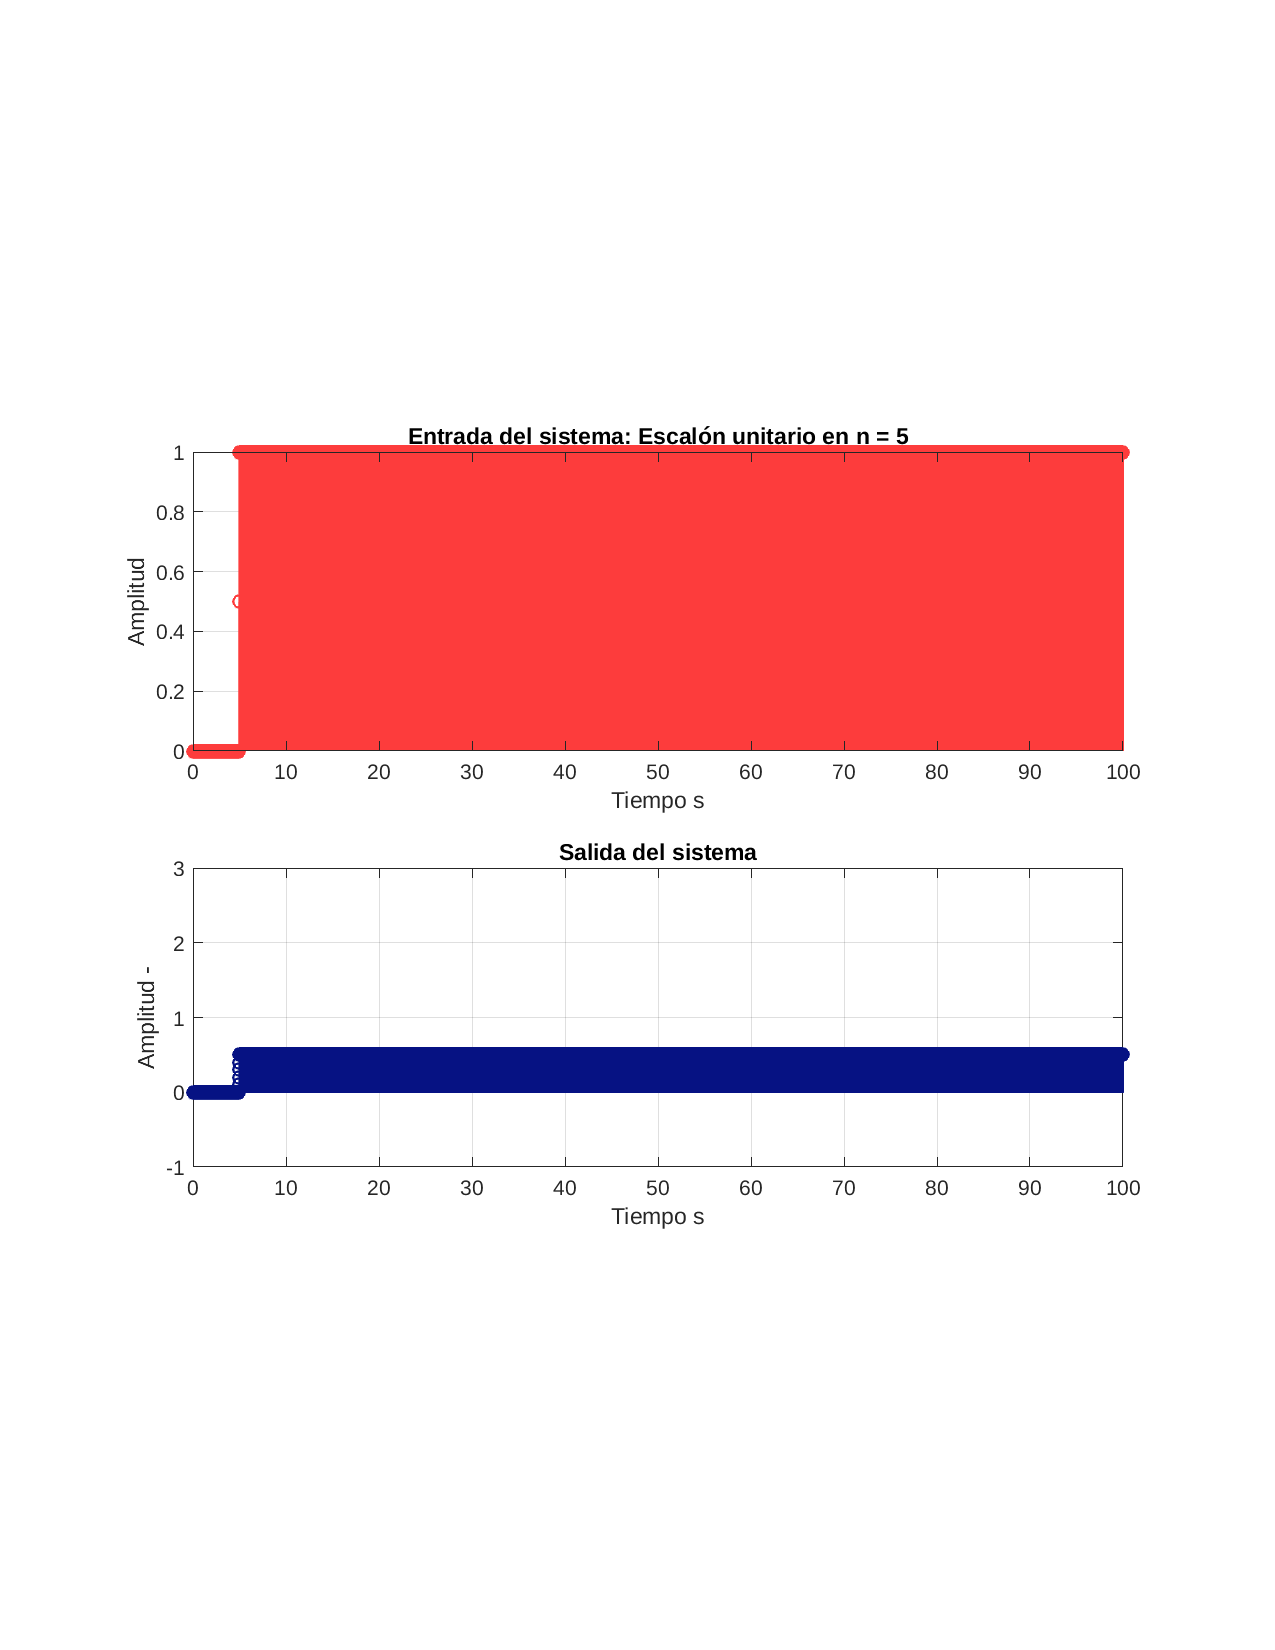
\includegraphics[width=0.6\textwidth,clip, trim = {2cm 7.0cm 2.2cm 7.0cm}]{../imgs/sistema_3_bibo_heaviside_n_5.pdf}
				\caption{Sistema \#3, para una entrada de escalón unitario, activado en n = 5 \textbf{(Arriba}}, para el cual se tiene la siguiente respuesta \textbf{(Abajo)}. 
				\label{fig:s_3_bibo_heaviside_n_5}
			\end{figure}
		
			Para esta salida,la respuesta del sistema es similar a la anterior, lo que da para especular, que el sistema mantiene la entrada que recibe, para este entrada el sistema nuevamente es estable. Siguiendo con la última señal de prueba, una señal triangular de amplitud 1 y frecuencia 1 \textit{Hz}: 
			\begin{figure}[H]
				\center
				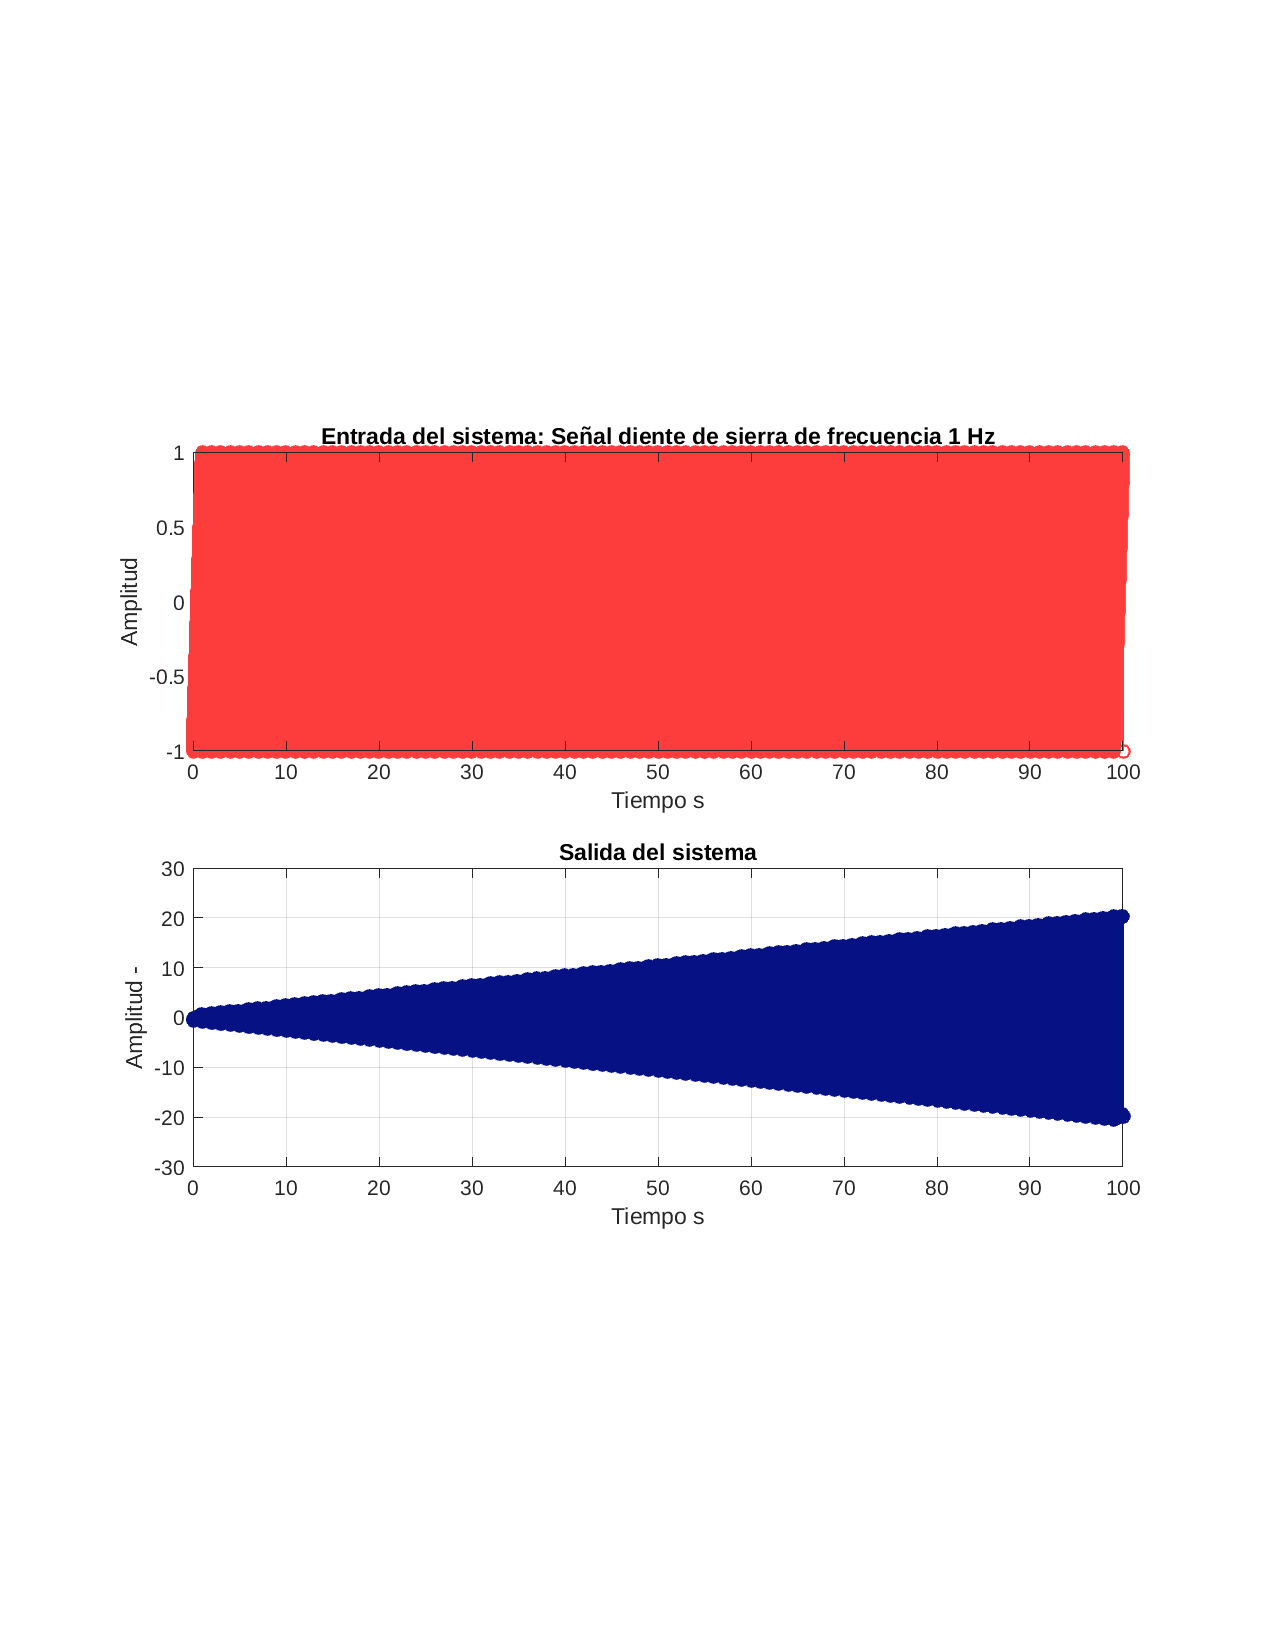
\includegraphics[width=0.6\textwidth,clip, trim = {2cm 7.0cm 2.2cm 7.0cm}]{../imgs/sistema_3_bibo_sawtooth.pdf}
				\caption{Sistema \#3, para una entrada de señal triangular \textbf{(Arriba)}, se tiene la siguiente salida \textbf{(Abajo)}.}
				\label{fig:s_3_bibo_sawtooth}
			\end{figure}
		
			Para esta entrada, el sistema tiende a amplificarse, lo que da pie a asumir, que la salida no será acotada. Por lo que se puede decir que el sistema \textbf{no es estable}.
			
	\subsection{Resumen}
		Resumiendo los resultados hallados en una tabla:
		\begin{table}[H]
			\center
			\begin{tabular}{|c|c|c|c|}
				\hline
				\textbf{Criterio} & \textbf{S1} & \textbf{S2} & \textbf{S3} \\
				\hline
				\textbf{Invariancia temporal} & No & Si & Si \\
				\hline
				\textbf{Linealidad} & Si & No & Si \\
				\hline
				\textbf{Estabilidad BIBO} & No & Si & No \\
				\hline			
			\end{tabular}
			\caption{Resumen de las características de los sistemas}
			\label{tab:summary_systems}
		\end{table}

\section{Inversión de Sistemas}
	Sea
	\begin{align}
		y = S_{a}(x) \\
		y[n] = \frac{1}{2}y[n-1]-x[n]
		\label{eq:considerations_system_inversion}
	\end{align}
	\subsection{Encontrar el sistema inverso}
		Buscamos obtener
		\begin{align}
			\delta[n] = S_{b}(S_{a}(\delta[n]))
			\label{eq:system_inverse_target}
		\end{align}
		
		Para encontrar el sistema $S_{b}$ que satisface lo anterior, es conveniente expresar la ecuación \ref{eq:considerations_system_inversion}, mediante su función de transferencia, aplicamos transformada Zeta:
		\begin{align}
			Y[z] = \frac{1}{2}Y[z]Z^{-1} - X[z] \\
			Y[z] \left( 1 - \frac{1}{2}Z^{-1} \right) = -X[z] \\
			H_{a}[z] = \frac{Y[z]}{X[z]} = \frac{2Z}{1 - 2Z}
			\label{eq:transfer_function_ha}
		\end{align}
		

		Con esta función de transferencia, buscamos que al aplicar ambos sistemas a una señal de entrada, el resultado sea la misma señal de entrada, esto equivale a poner ambos a poner ambos sistemas en cascada:
		\begin{equation}
			S_{b}(S_{a}(x[n])) \equiv h_{b}[n] * h_{a}[n] * x[n] = x[n]
		\end{equation}
		
		En términos de la transformada Zeta:
		\begin{equation}
			H_{a}[z] \cdot H_{b}[z] \cdot X[z] = X[z] \Longleftrightarrow H_{a}[z] \cdot H_{b}[z] = 1
 		\end{equation}
 		
 		Por lo que podemos definir:
 		\begin{equation}
 			\boxed{H_{b}[z] = \frac{1}{H_{a}[z]} = \frac{1 -2Z}{2Z}}
 		\end{equation}
 		
 		De esta forma, encontramos la respuesta a impulso que debe tener el sistema inverso, volviendo a ecuaciones en diferencia, expresamos el sistema:
 		\begin{equation}
 			\boxed{y[n] = -x[n] + \frac{1}{2}x[n-1]}
 			\label{eq:2_inverse_system}
 		\end{equation}
 		
 	\subsection{Implementación en Matlab}
 		Implementando ambos sistemas como funciones en Matlab:
 		
 		\begin{figure}[H]
 			\lstinputlisting[language=Matlab, firstline=49, lastline=61]{../parte_ii.m}
 		\end{figure}
 		
 		\subsubsection{Respuesta a impulso de Sa(x)}
 			\begin{figure}[H]
 				\center
 				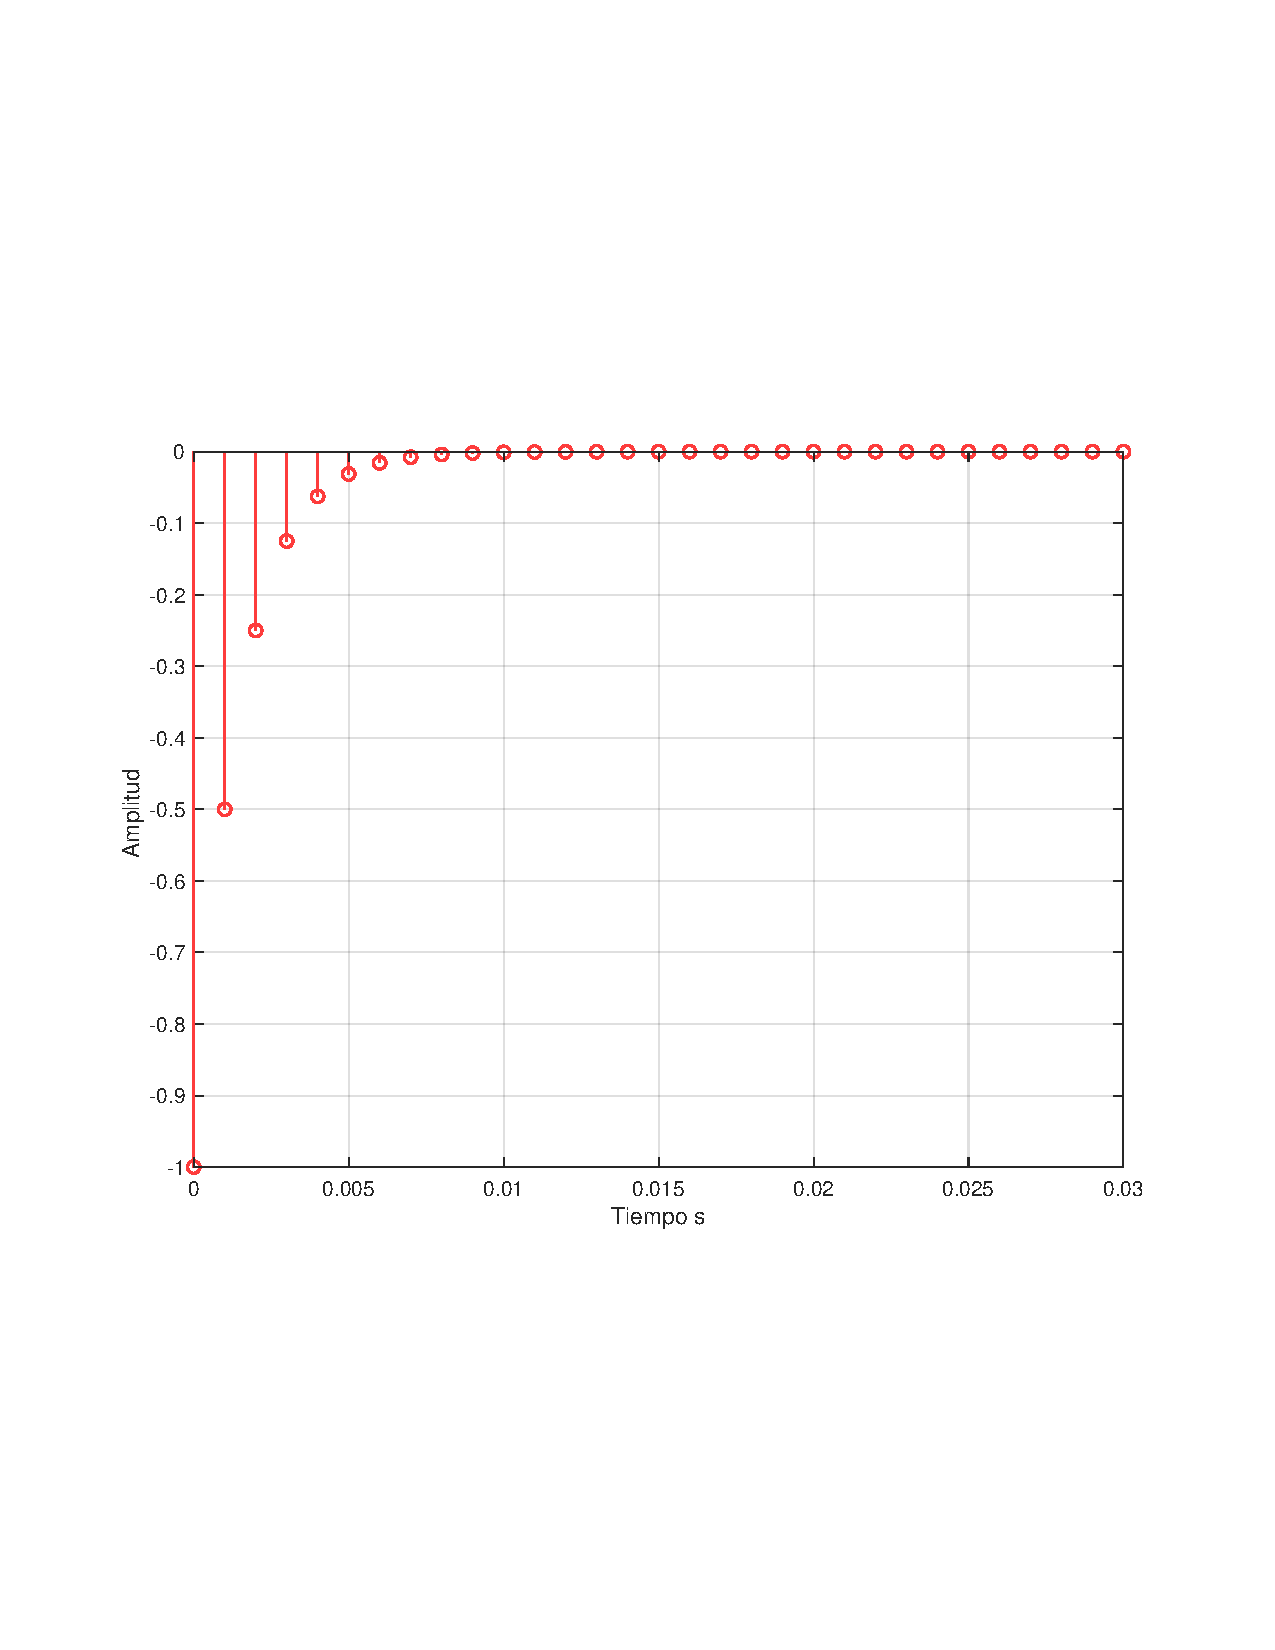
\includegraphics[width=0.6\textwidth,clip, trim = {2cm 7.0cm 2.2cm 7.0cm}]{../imgs/2_Sa.pdf}
				\caption{Respuesta del sistema $S_{a}(x)$ a impulso}
 				\label{fig:2_Sa}
 			\end{figure}
			Analizando la respuesta de este sistema, podemos comprobar lo descrito en la ecuación \ref{eq:considerations_system_inversion}, el valor actual de la salida, corresponde a 0.5 el valor anterior de la salida, menos el valor actual. Como el delta solo se aplica en t = 0, la salida parte con un valor negativo y se va reduciendo por un factor de 0.5 a medida que avanza el tiempo. 
			
 		\subsubsection{Respuesta a impulso de Sb(x)}
 			\begin{figure}[H]
 				\center
 				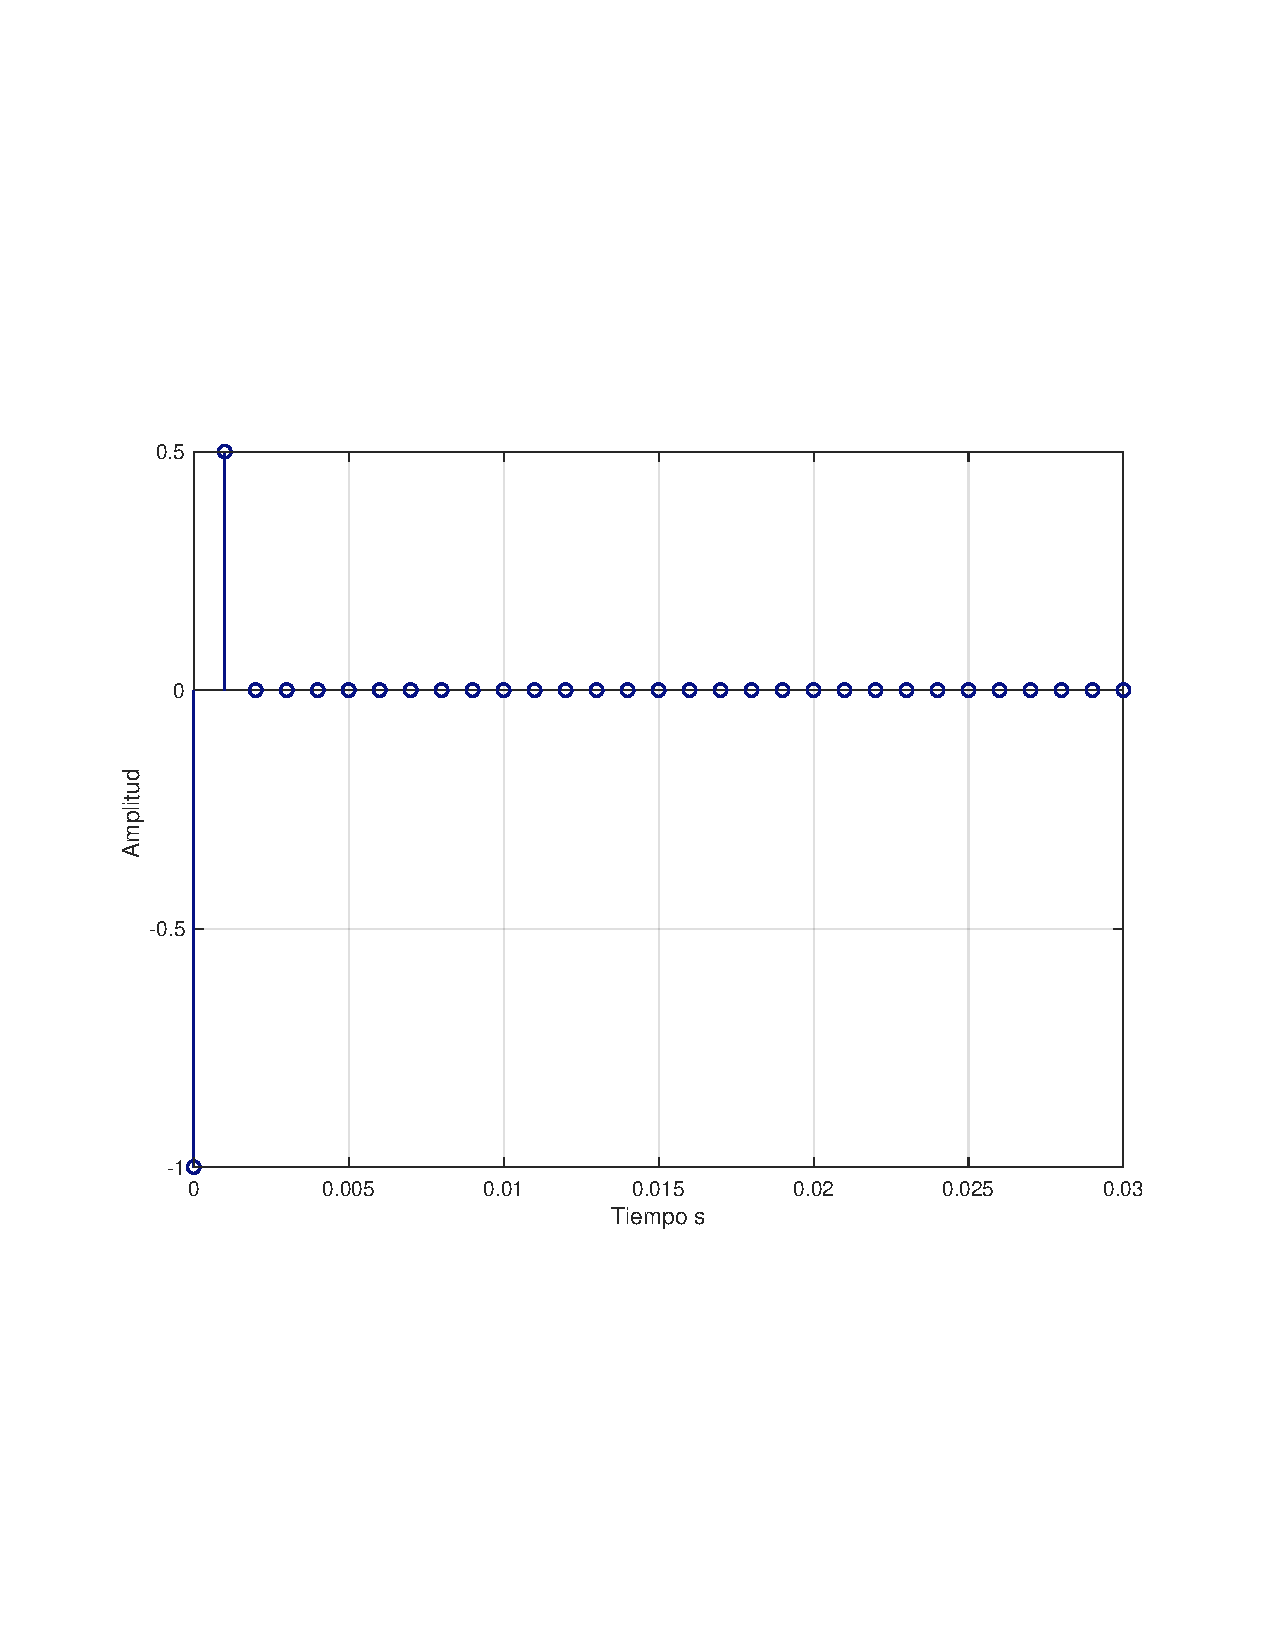
\includegraphics[width=0.6\textwidth,clip, trim = {2cm 7.0cm 2.2cm 7.0cm}]{../imgs/2_Sb.pdf}
				\caption{Respuesta del sistema $S_{b}(x)$ a impulso}
 				\label{fig:2_Sb}
 			\end{figure}
 			
 			Comparando el resultado con lo esperado con la ecuación \ref{eq:2_inverse_system}, notamos que el sistema toma el valor actual de la salida, escalado por -1 y 0.5 veces el valor anterior de la entrada, es por esto que con un delta en t = 0  como entrada,  la salida primero se dispara a -1 (la señal anterior a t = 0 es 0), para al siguiente instante, tomar valor 0.5 y al siguiente mantenerse en cero. 
		\subsubsection{Respuesta a impulso de Sb(Sa(x))}
 			\begin{figure}[H]
 				\center
 				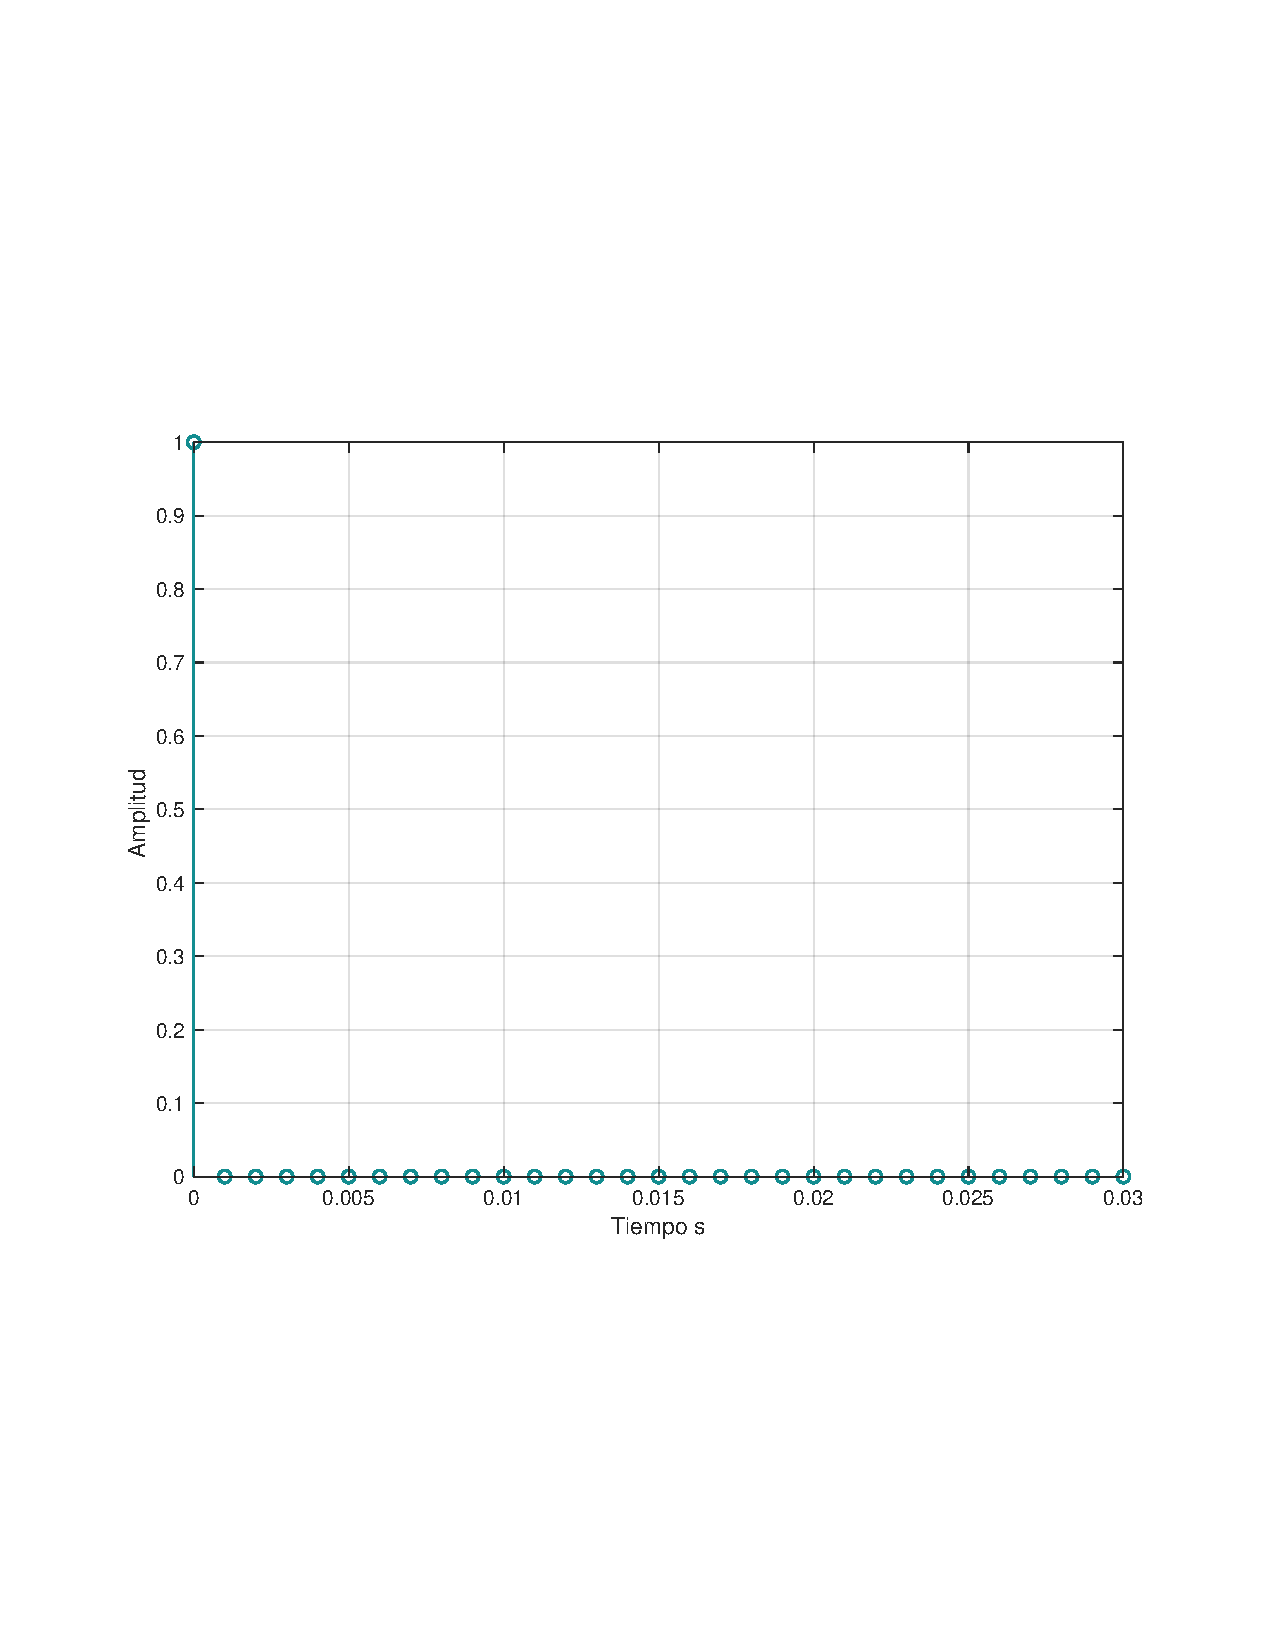
\includegraphics[width=0.6\textwidth,clip, trim = {2cm 7.0cm 2.2cm 7.0cm}]{../imgs/2_SbSa.pdf}
				\caption{Respuesta del sistema $S_{b}(S_{a}(x))$ a impulso}
 				\label{fig:2_SbSa}
 			\end{figure}
 			
 			Como se esperaba, dado que las funciones de transferencia son complementarias, el resultado es la misma señal de entrada.
 			
\section{Integrales y derivadas en tiempo discreto}
	Se considera, para tiempo continuo:
	\begin{align}
		y = S_{1}(x) \text{tal que } y(t) = \frac{d}{dt}x(t) \\
		y = S_{2}(x) \text{tal que } y(t) = \int_{-\infty}^{t} x(\tau)d\tau
	\end{align}
	
	\subsection{Aproximaciones de tiempo discreto}
		\subsubsection{Derivada}
			Consideremos la definición formal de la derivada temporal
			\begin{equation}
				\frac{d}{dt}x(t) = \lim_{h \rightarrow 0} \frac{x(t + h) + x(t)}{h}
				\label{eq:derivative_def} 
			\end{equation}
			
			Podemos realizar un análogo casi directo para tiempo continuo, considerando que la muestra $n-1$ y la muestra $n$, están separadas temporalmente por $T_{s}$. Expresando esto:
			\begin{equation}
				\frac{\Delta x[n]}{\Delta t} = \frac{x[n] - x[n-1]}{T_{s}} \approx \frac{d}{dt}x(t) |_{t = n}
			\end{equation}
			
			Llevando la expresión hallada a una forma de sistema:
			\begin{equation}
				\boxed{y[n] = \frac{x[n] - x[n-1]}{T_{s}}}
				\label{eq:derivative_S1}
			\end{equation}
			
			Analizando esta expresión, notemos que mientras la señal x[n] sea acotada y no presente \textit{saltos}, la salida y[n] será acotada, por lo que el sistema es \textbf{BIBO estable}. Notemos que esta aproximación de la derivada no es única, por ejemplo, se podría haber calculado como la diferencia entre la muestra n+1 y la muestra n, llegando al mismo resultado.
			
		\subsubsection{Integral}
			Considerando la definición por sumas de Riemann, de la integral:
			\begin{equation}
				\int_{a}^{b} f(x)dx =  \lim_{\Delta_{i} \rightarrow 0} \sum_{i = 1}^{n} f(t_{i}) \Delta_{i}
			\end{equation}			 
			
			Descomponiendo el término de la sumatoria, lo que obtenemos es que la suma del rectángulo de base $\Delta_{i}$ y altura $f(t_{i})$, con los rectángulos que le precedieron. Considerando que $\Delta_{i} = T_{s}$, podemos expresar esta idea en términos de ecuaciones de diferencia:
			\begin{equation}
				\boxed{y[n] = y[n-1] + T_{s}x[n]}
			\end{equation}
			
			La salida, está definida por el valor anterior de la salida y el área formada por el rectángulo de base $T_{s}$ y altura x[n]. Podemos saber que este sistema \textbf{no es BIBO estable}, considerando el caso donde se ingresa un escalón unitario a un integrador, ésta señal es acotada, pero si tendemos $t \rightarrow \infty$, el área bajo la curva, tenderá a ser infinita. 
			
	\subsection{Análisis con señal sinusoidal}
		Se considera una frecuencia de muestreo $f_{s} = 10$ \textit{KHz}. Consideramos una señal de prueba de las siguientes características:
		\begin{equation}
			x(t) =  \sin(2\pi\cdot 100 t)
		\end{equation}
		
		\begin{figure}[H]
			\center
			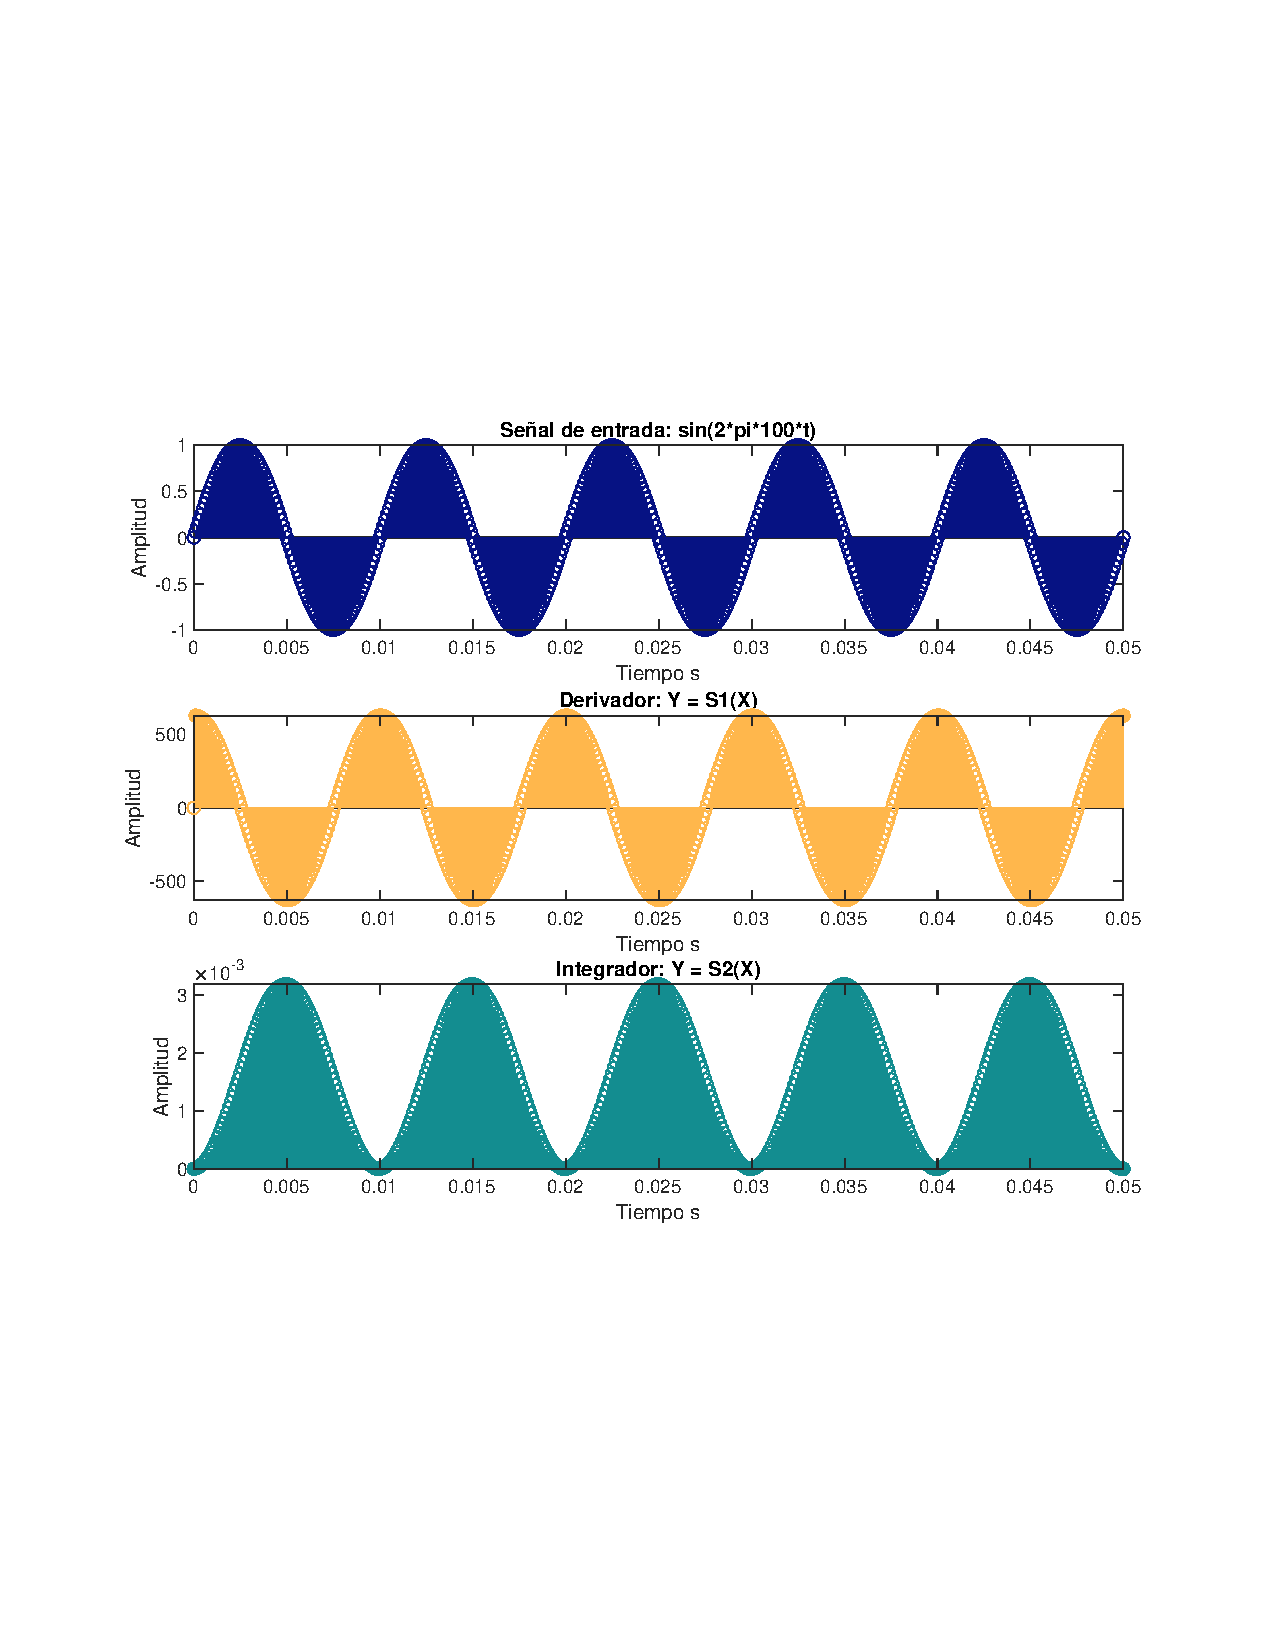
\includegraphics[width=0.6\textwidth,clip, trim = {2cm 7.0cm 2.2cm 7.0cm}]{../imgs/3_b.pdf}
			\caption{Resultado para la señal de entrada, en términos de su derivada e integral}
			\label{fig:3_b}
		\end{figure}
		
		Para el caso de la derivada, calculamos el valor esperado de manera teórica:
		\begin{equation}
			\frac{d}{dt}x(t) = 200\pi \cdot cos(200\pi t)
		\end{equation}
		
		Observando el resultado gráfico, notamos que la señal obtenida a la salida de S1(x), está desfasada en $\pi/2$ con respecto a la señal original, lo que nos permite concluir que es un coseno. Analizando la amplitud, se puede estimar que está acotada en un valor $|627| \approx 200\pi$ lo que corresponde con la expresión teórica para la derivada de un seno. 
		
		Para el caso de la integral, el valor esperado de manera teórica:
		\begin{equation}
			\int sin(200\pi t) dt = \frac{-1}{200\pi} cos(200\pi t) + C
		\end{equation}
		
		Considerando que el valor inicial en t = 0, será cero:
		\begin{align}
			C = \frac{1}{200\pi} \\
			\therefore \int sin(200\pi t) dt = \frac{-1}{200\pi} cos(200\pi t) + \frac{1}{200 \pi}
		\end{align}
		
		Notamos que el resultado gráfico, corresponde a lo esperado, dado que a medida que la señal avanzan en un período, el área bajo la curva, incrementa hasta alcanzar un máximo, para luego retornar a cero al cumplirse un período. El valor máximo que alcanza el área es $0.032$, que corresponde al caso donde se cumple medio periodo de la señal, valor que corresponde a lo esperado de manera teórica. 
	\subsection{Derivada e integral de: composicion de deltas}
		Se define la señal de entrada como:
		\begin{equation}
			x[n] = \delta [n] - \delta [n-5] 
		\end{equation}
		
		\begin{figure}[H]
			\center
			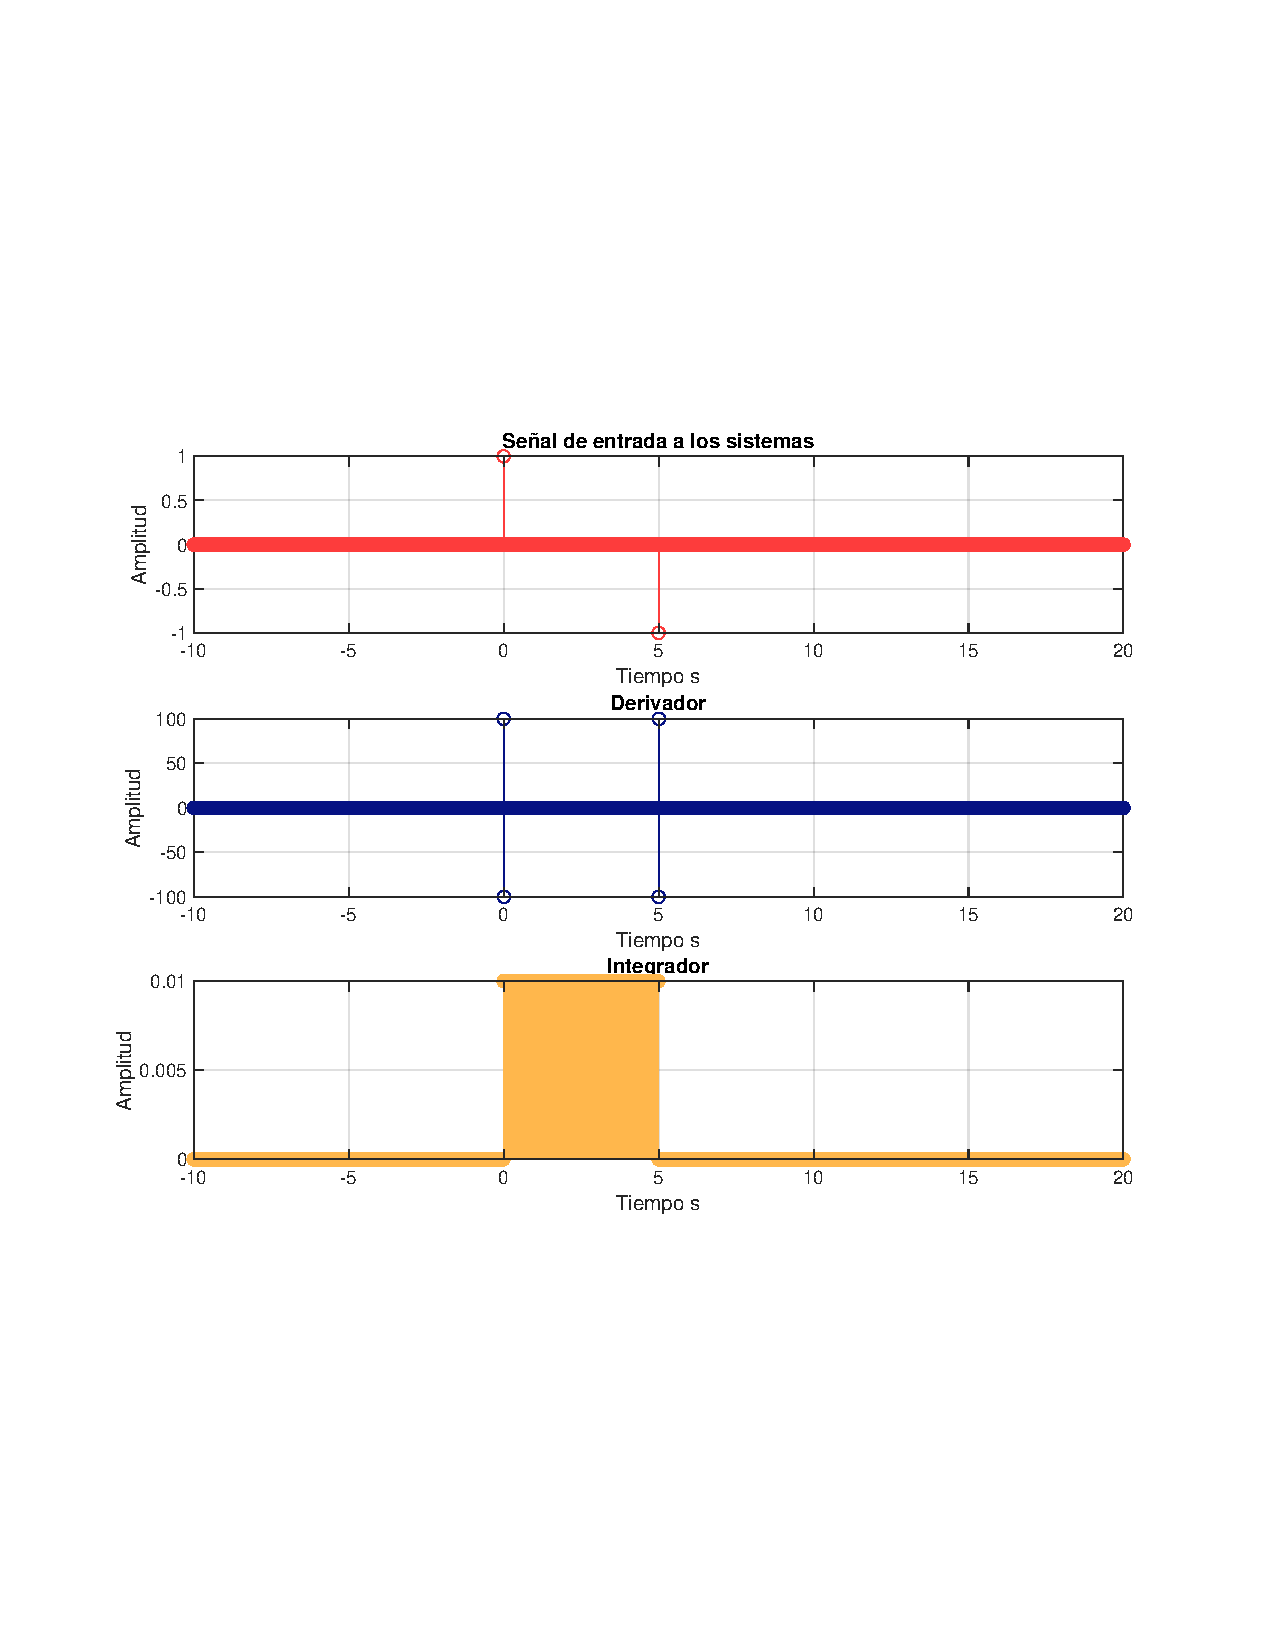
\includegraphics[width=0.6\textwidth,clip, trim = {2cm 7.0cm 2.2cm 7.0cm}]{../imgs/3_c.pdf}
			\caption{Resultado para la señal de entrada, en términos de su derivada e integral}
			\label{fig:3_c}
		\end{figure}
		
		Analizando los resultados, notemos que son coherentes a lo que se obtendría de manera teórica. Para el caso de la derivada, consideremos lo que pasa cuando nos acercamos al delta, estamos en valores de la señal de entrada que son cero. Cuando se llega al delta, la derivada se definira como la diferencia entre un valor muy alto y un valor cero, el cual será positivo, lo que da como salida un delta con valor positivo. A medida que nos alejamos del delta, esta diferencia ahora será entre un valor cercano a cero y un valor muy grande, lo cual arrojara un delta negativo. En el caso de la integral, es conocido que la integral de un delta corresponde a un escalón unitario.
	\subsection{Derivada e integral de: composición de escalones unitarios}
		 Se define la señal de entrada como:
		\begin{equation}
			x[n] = \mu [n] - \mu [n-5] 
		\end{equation}
		
		\begin{figure}[H]
			\center
			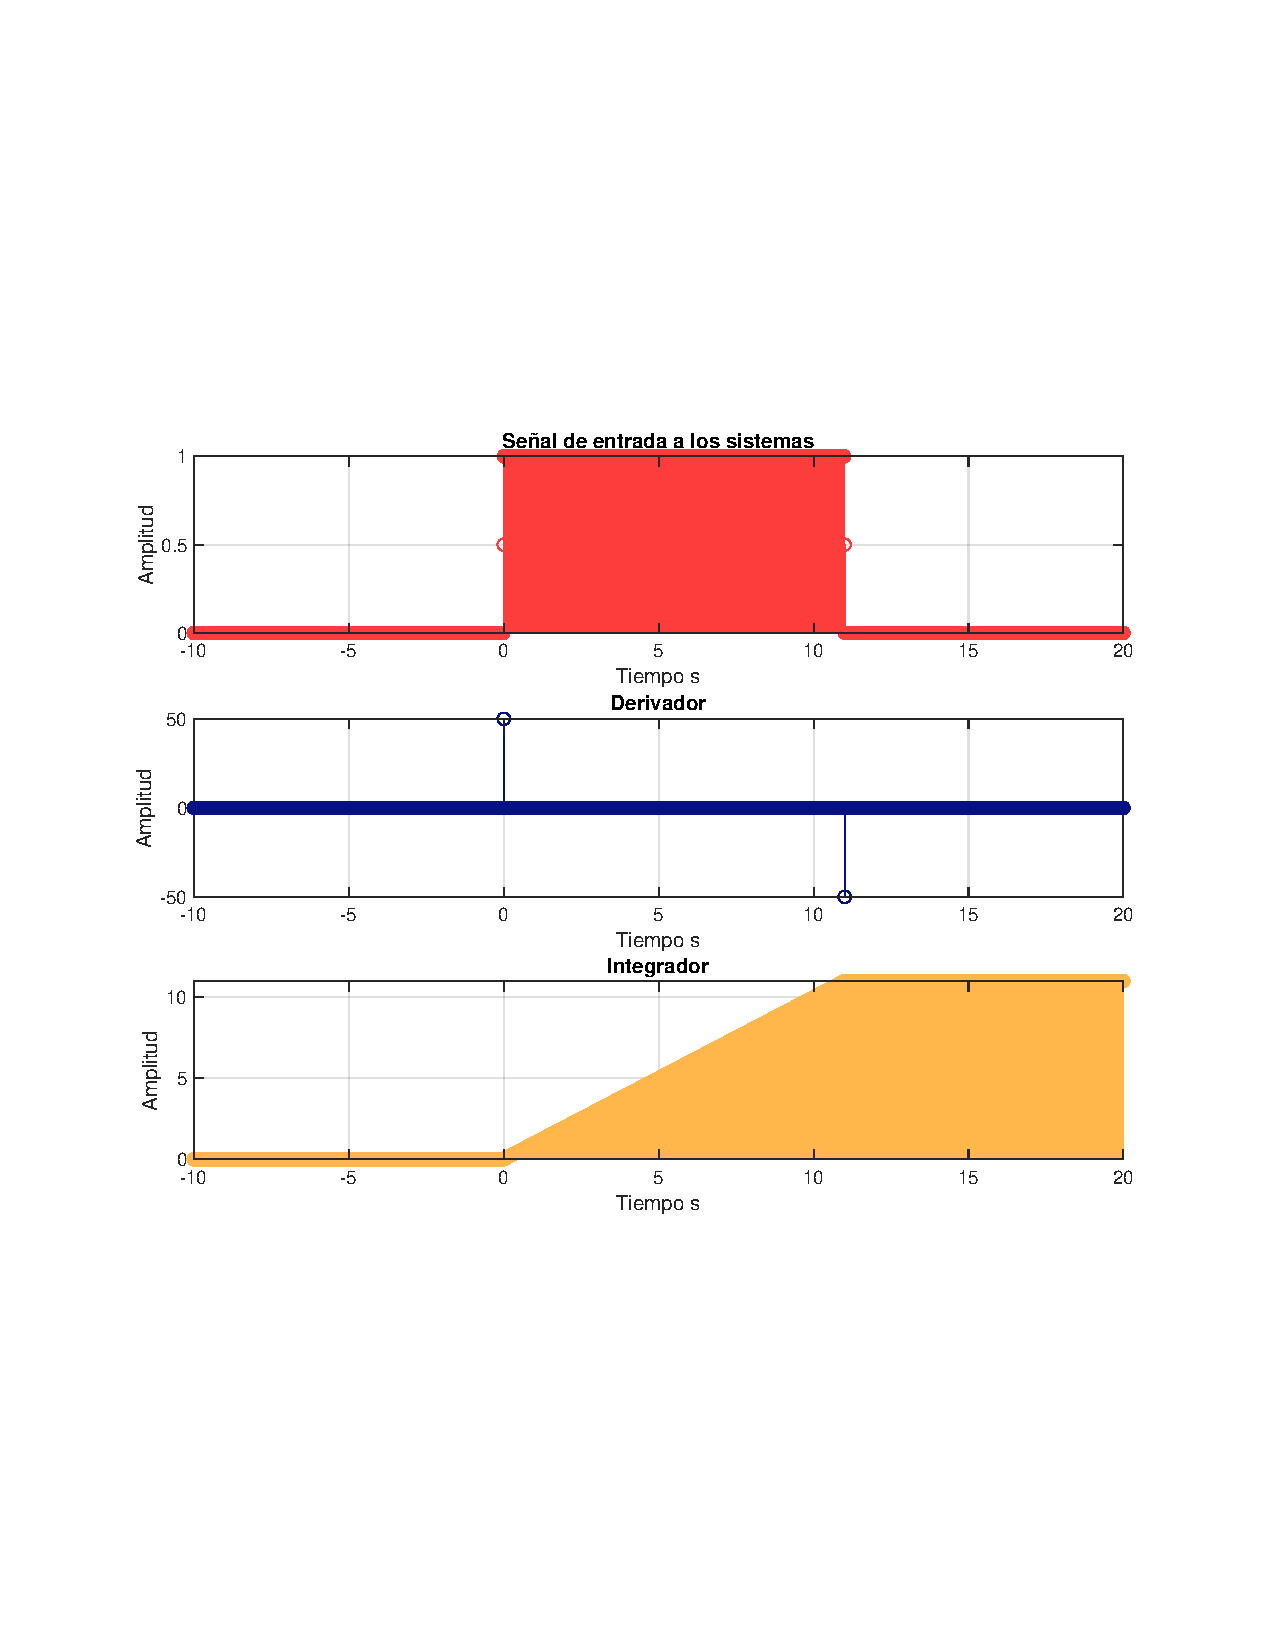
\includegraphics[width=0.6\textwidth,clip, trim = {2cm 7.0cm 2.2cm 7.0cm}]{../imgs/3_d.pdf}
			\caption{Resultado para la señal de entrada, en términos de su derivada e integral}
			\label{fig:3_d}
		\end{figure}
		
		Nuevamente el resultado es lo esperado, al derivar la composición de escalones, se obtendrá por definición dos deltas. En el caso de la integración, se obtendrá una señal que aumenta en amplitud junto con el área, hasta que se activa el segundo escalón que hace que el área se vuelva constante, por lo tanto la salida también. 
		
	\subsection{Derivada e integral de señales de audio}
		\subsubsection{Derivada}
			Al pasar la señales por el sistema de derivación, se siente que sólo quedan las componentes de alta frecuencia al escuchar la señal. Esto se debe a que la derivada actua como un filtro pasa altos, las componentes de menos frecuencia son atenuadas mientras que las señales con componentes de frecuencia altas pasan sin ser afectadas.
		\subsubsection{Integral}
			Este sistema se comporta de manera inversa al anterior, la integral actúa como un filtro pasabajos, componentes espectrales de baja frecuencia tienen un mayor efecto que componentes de frecuencia más alta, por esto al escuchar la señal esta se siente más apagada. 

	\subsection{Doble derivada y doble integral}
			Para poder determinar estos sistemas es conveniente expresar $S_{1}$ y $S_{2}$ mediante su función de transferencia en el dominio Zeta:
			\begin{align}
				H_{1}[z] = f_{s}\frac{z-1}{z} \\
				H_{2}[z] = \frac{1}{fs} \frac{z}{z-1} 
			\end{align}
			
			Se puede considerar cada una de estas funciones como un filtro, por lo que para conseguir la segunda derivada o integral, basta con poner los filtros en cascada.
			\subsubsection{Doble derivada S1(S1(x))}
				\begin{equation}
					\frac{d}{dt}x(t)|_{n} \approx h_{1}[n] * h_{1}[n]
				\end{equation}
				
				En el dominio de la transformada zeta:
				\begin{equation}
					H_{11}[z] = f_{s}^{2} \frac{z^{2} -2z + 1}{z^{2}}
				\end{equation}
				
				Como ecuación de diferencias:
				\begin{equation}
					y[n] = \left( x[n] - 2x[n-1] + x[n-2] \right) f_{s}^{2}
				\end{equation}
				
				Para este caso,  se tiene que mientras la señal de entrada sea acotada, la salida también lo será, por lo que el sistema es \textbf{BIBO estable}. El sistema se comporta como un filtro pasa-altos.
				
			\subsubsection{Doble derivada S2(S2(x))}
				\begin{equation}
					\int_{-\infty}^{t}\int_{-\infty}^{r}x(\tau)d\tau \approx h_{2}[n] * h_{2}[n]
				\end{equation}
				
				En el dominio de la transformada zeta:
				\begin{equation}
					H_{22}[z] = \frac{1}{f_{s}^{2}} \frac{z^{2}}{z^{2} -2z + 1}
				\end{equation}
				
				Como ecuación de diferencias:
				\begin{equation}
					y[n] = \frac{1}{f_{s}^{2}} x[n] + 2y[n-1] - y[n-2]
				\end{equation}
				
				Como se demostró anteriormente la integral es un sistema inestable, por lo que la doble integral también es \textbf{inestable}. Este sistema se comporta como un filtro pasabajos. 
				
			\subsubsection{Derivada de una integral e integral de una derivada}
				Note que ambos sistemas son análogos, sabiendo que son operaciones recíprocas (sus funciones de transferencia son recíprocas), el efecto de poner cualquier permutación de estos filtros será la misma:
				\begin{equation}
				H_{1}[z] \cdot H_{2}[z] = H_{2}[z] \cdot H_{1}[z] = 1 
				\end{equation}
				
				El sistema se comporta de manera transparente, la entrada es igual a la salida. La estabilidad estará dada únicamente por la estabilidad de la entrada.
\section{Radar}
	Considere:
	\begin{align}
		y_{a} = ax_{a}(t-t_{d}) + v_{a}(t) \\
		x[n] = x_{a}[nT_{s}] \\
		y[n] = ax_{a}[nT_{s}] + v_{a}[nT_{s}] = ax[n-D] + v[n]
	\end{align}
	\subsection{Obtención del retardo D}
		Sea la correlación cruzada:
		\begin{equation}
			r_{xy}[n] = \sum_{k=-\infty}^{\infty} x[k] \cdot y[n+k] = x[n]*y[n]
		\end{equation}
		
		Usando esta definición se puede obtener que la máxima correlación se obtendrá cuando las señales sean lo más parecidas posibles dado que la multiplicación será máxima. Aplicando esto a las señales del sistema dado:
		\begin{equation}
			r_{yx}[n] = \sum_{k=-\infty}^{\infty} y[n] \cdot x[n-k]  \equiv \sum_{k=-\infty}^{\infty} \left( ax[n-D] + v[n] \right)  \cdot x[n-k] 
		\end{equation}
		
		El valor máximo para la correlación ocurrirá cuando $k = D$. De esta forma, buscando cuando ocurre el máximo se puede estimar el valor del desfase entre las señales. Consideremos la correlación de la señal que vuelve al radar sobre sí misma:
		\begin{equation}
			r_{yy}[n] = \sum_{k=-\infty}^{\infty} y[n] \cdot y[n-k]  \equiv \sum_{k=-\infty}^{\infty} \left( ax[n-D] + v[n] \right)  \cdot \left( ax[n-D-k] + v[n-k] \right)
		\end{equation}
		
		Para este caso, no se puede extraer información acerca del retraso D, dado que el máximo valor se obtendrá para k = 0.
	\subsection{Simulación con parámetros a = 0.9 , D= 20}
		\begin{figure}[H]
			\center
			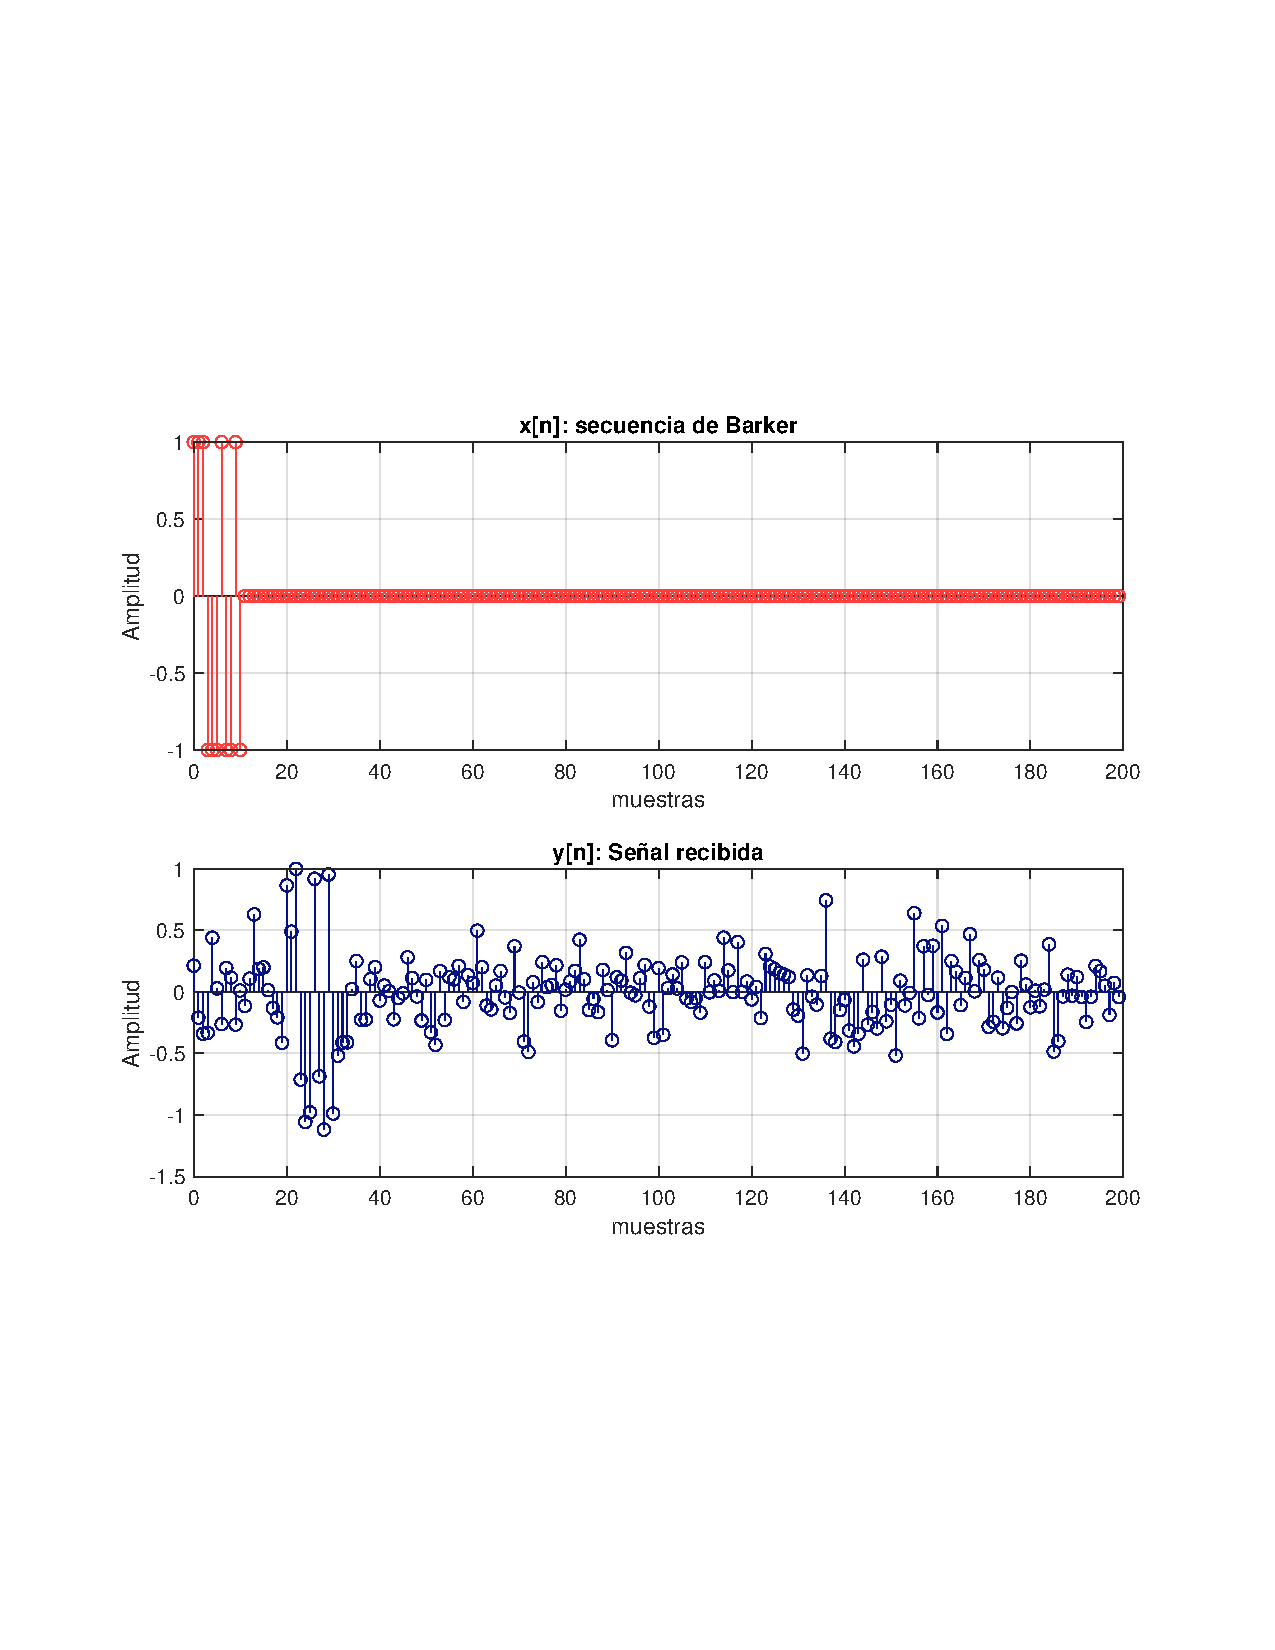
\includegraphics[width=0.6\textwidth,clip, trim = {2cm 7.0cm 2.2cm 7.0cm}]{../imgs/4_radar_b.pdf}
			\caption{Simulación de la situación}
			\label{fig:radar_b_sim}
		\end{figure}
		
		Pese al ruido, es posible encontrar la secuencia de barker reflejada.
		
	\subsection{Correlación ryy e ryx de la señal anterior}
		\begin{figure}[H]
			\center
			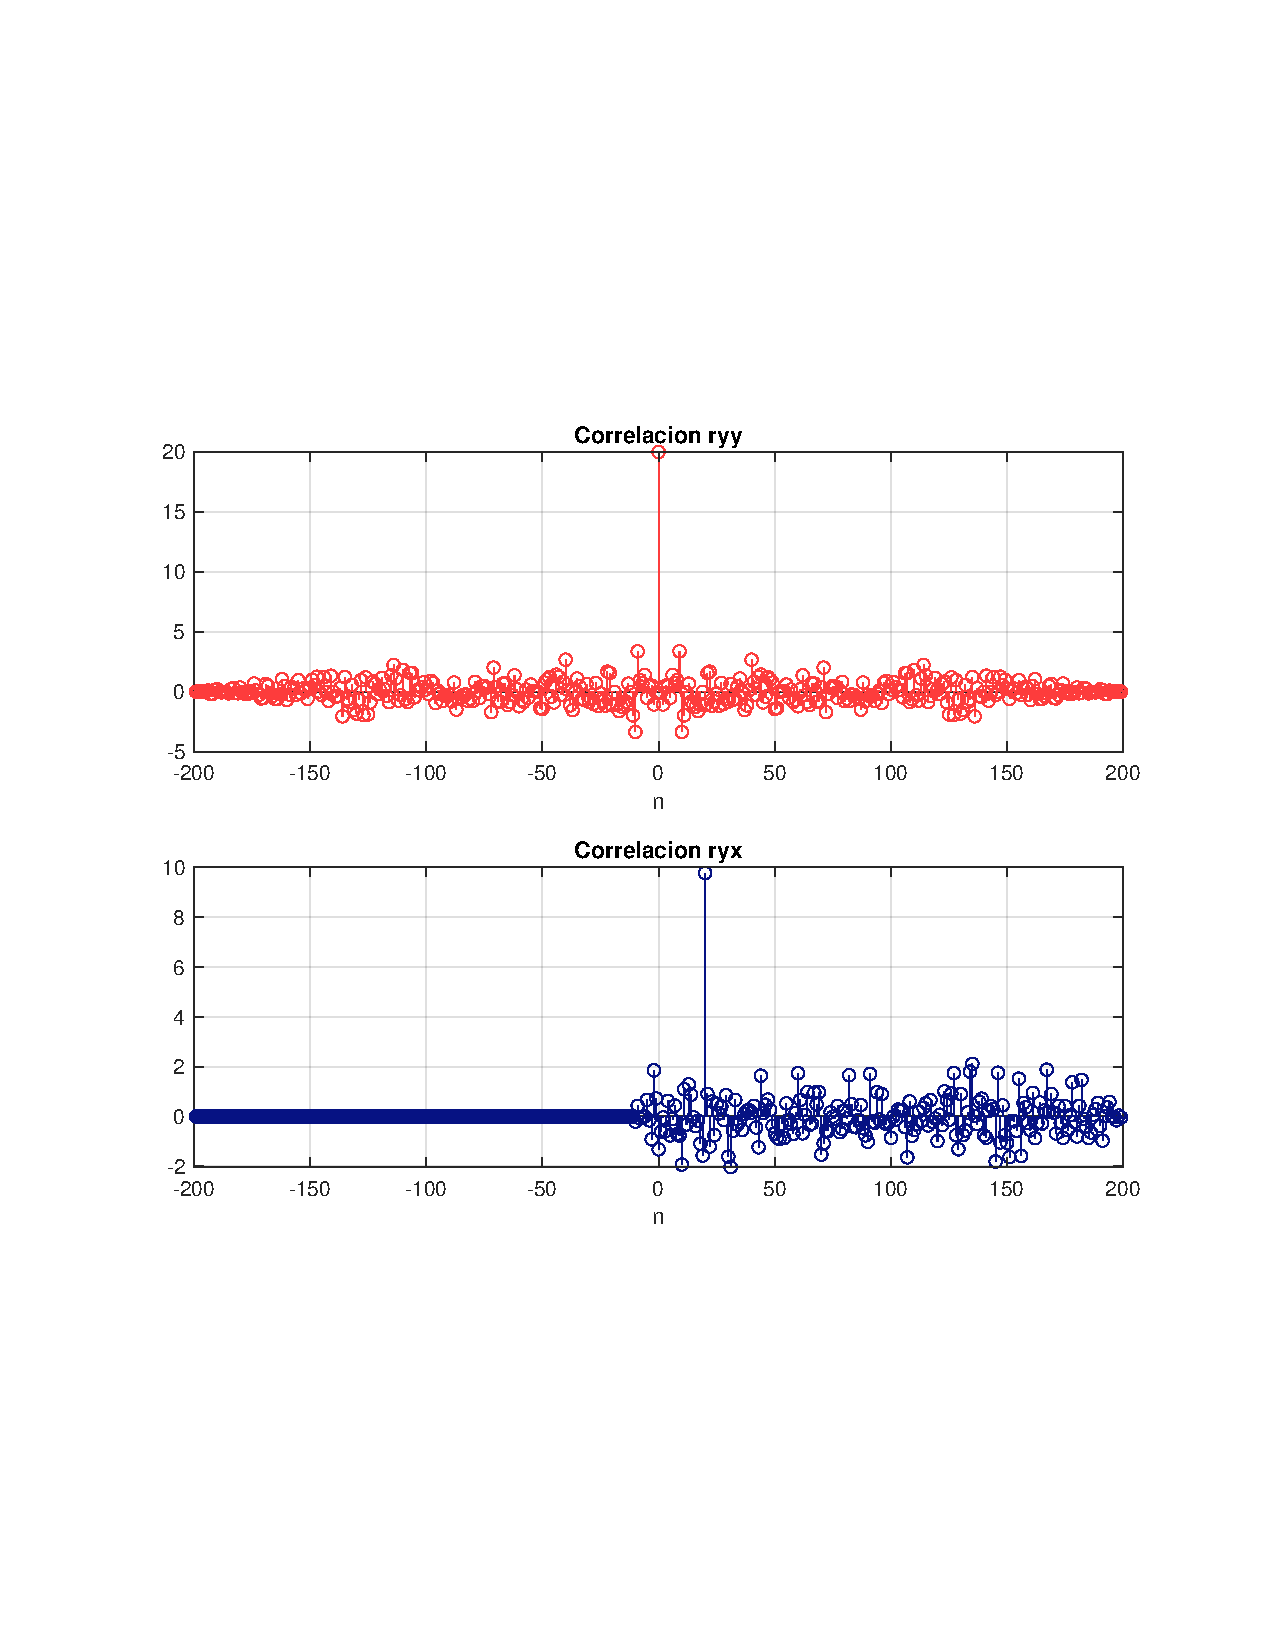
\includegraphics[width=0.6\textwidth,clip, trim = {2cm 7.0cm 2.2cm 7.0cm}]{../imgs/4_radar_c.pdf}
			\caption{Correlación ryy e ryx de la situación anterior}
			\label{fig:radar_c_ryy_ryx}
		\end{figure}
		
		A partir de estos gráficos es posible confirmar las predicciones hechas al momento de buscar una forma de encontrar el retardo. La correlación cruzada ryx, permite encontrar el retardo D, al observar el peak que esta presenta en n = 20. En cambio la correlación ryy no permite obtener el valor del retardo, dado que el peak ocurre en n = 0. Obteniendo el valor de SNR\footnote{Utilizando el comando correspondiente en Matlab}, se obtiene que la señal y[n] y el ruido están en una relación de 2.472 \textit{dB}. 
		
	 \subsection{Simulación con nuevos parámetros de ruido}
	 	\subsubsection{$\sigma^{2} = 0.1$}
	 		\begin{figure}[H]
			\center
			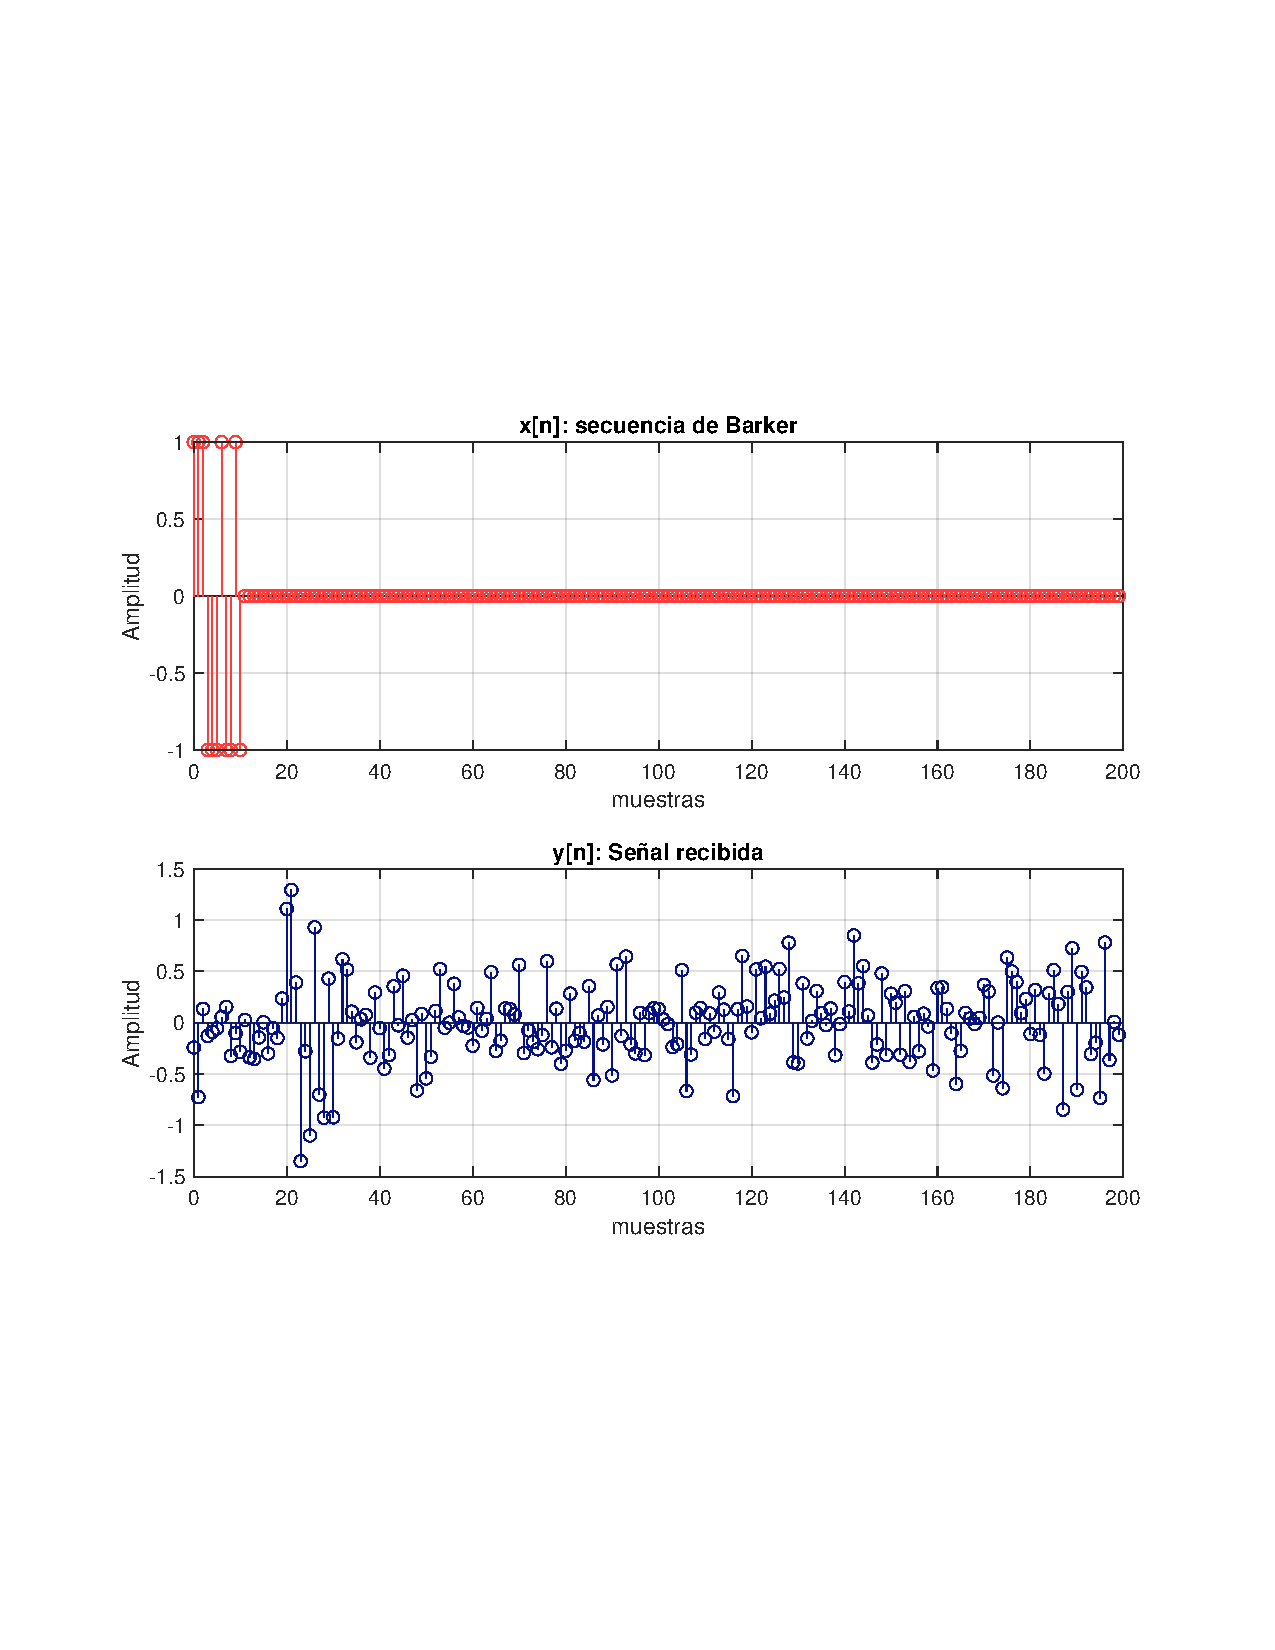
\includegraphics[width=0.6\textwidth,clip, trim = {2cm 7.0cm 2.2cm 7.0cm}]{../imgs/4_radar_d_0_1_signal.pdf}
			\caption{Simulación de la situación}
			\label{fig:radar_d_0_1_sim}
			\end{figure}	
			
			\begin{figure}[H]
			\center
			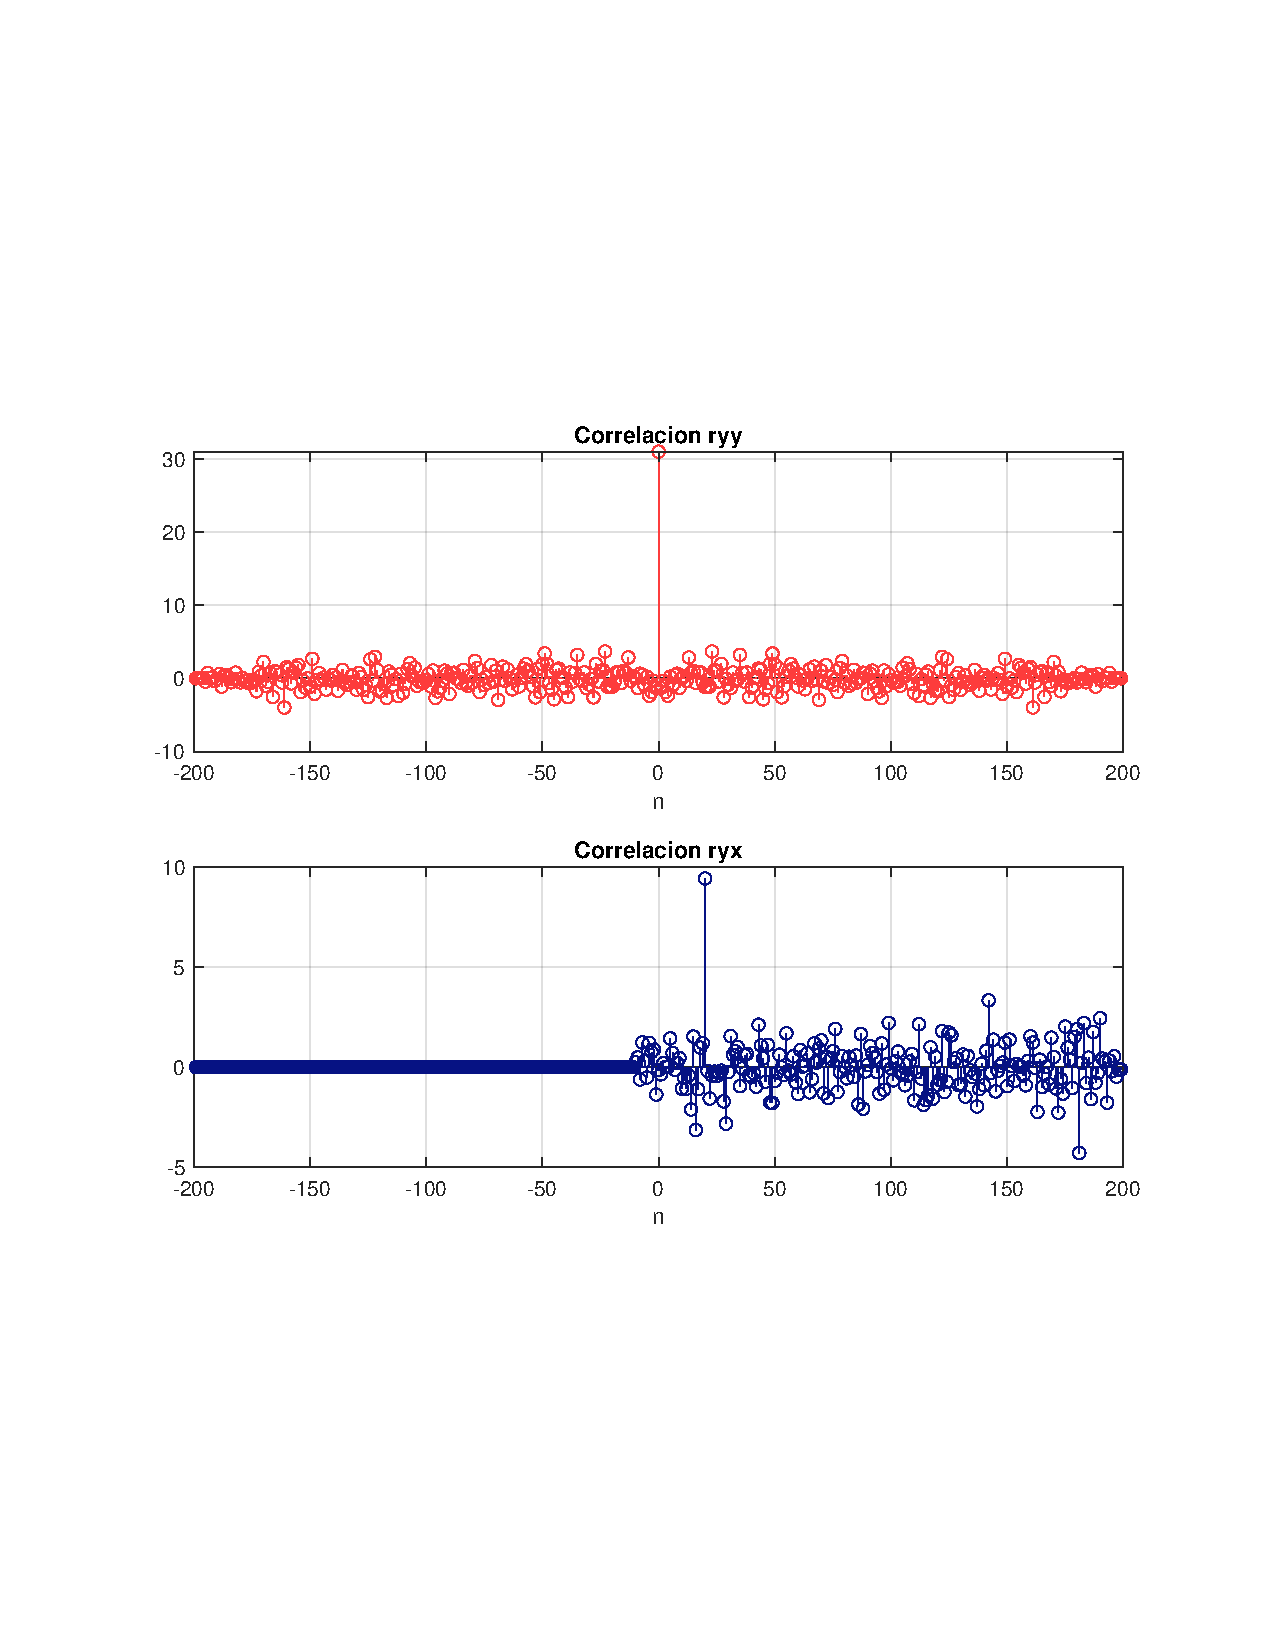
\includegraphics[width=0.6\textwidth,clip, trim = {2cm 7.0cm 2.2cm 7.0cm}]{../imgs/4_radar_d_0_1_corre.pdf}
			\caption{Correlación ryy e ryx de la situación anterior}
			\label{fig:radar_d_0_1_corre}
		\end{figure}
		
		Para este nuevo caso, se tiene un SNR de 1.30 \textit{dB}, lo que implica que al aumentar la variancia la señal se vuelve más suceptible al ruido. Sin embargo, la estimación del retraso sigue otorgando el mismo valor a partir de la correlación D = 20.
		
		\subsubsection{$\sigma^{2} = 1$}
	 		\begin{figure}[H]
			\center
			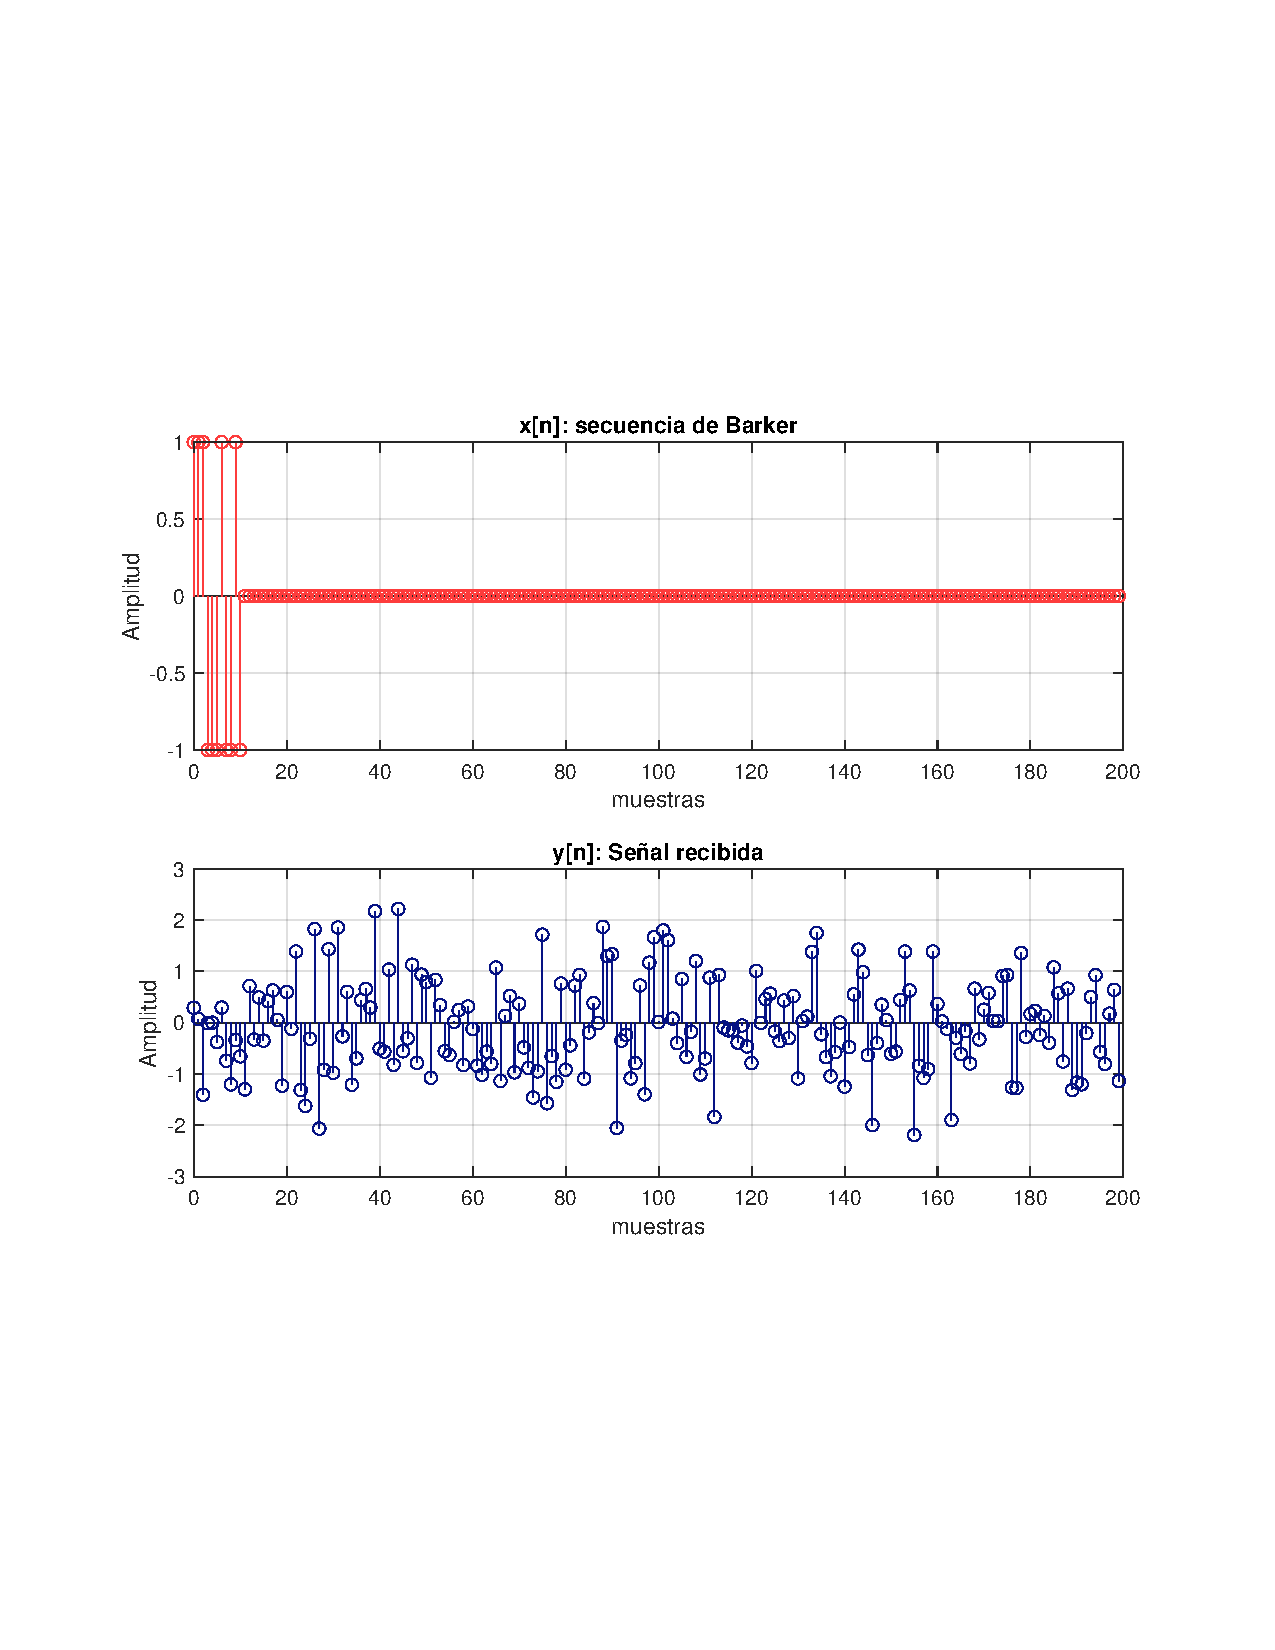
\includegraphics[width=0.6\textwidth,clip, trim = {2cm 7.0cm 2.2cm 7.0cm}]{../imgs/4_radar_d_1_signal.pdf}
			\caption{Simulación de la situación}
			\label{fig:radar_d_1_sim}
			\end{figure}	
			
			\begin{figure}[H]
			\center
			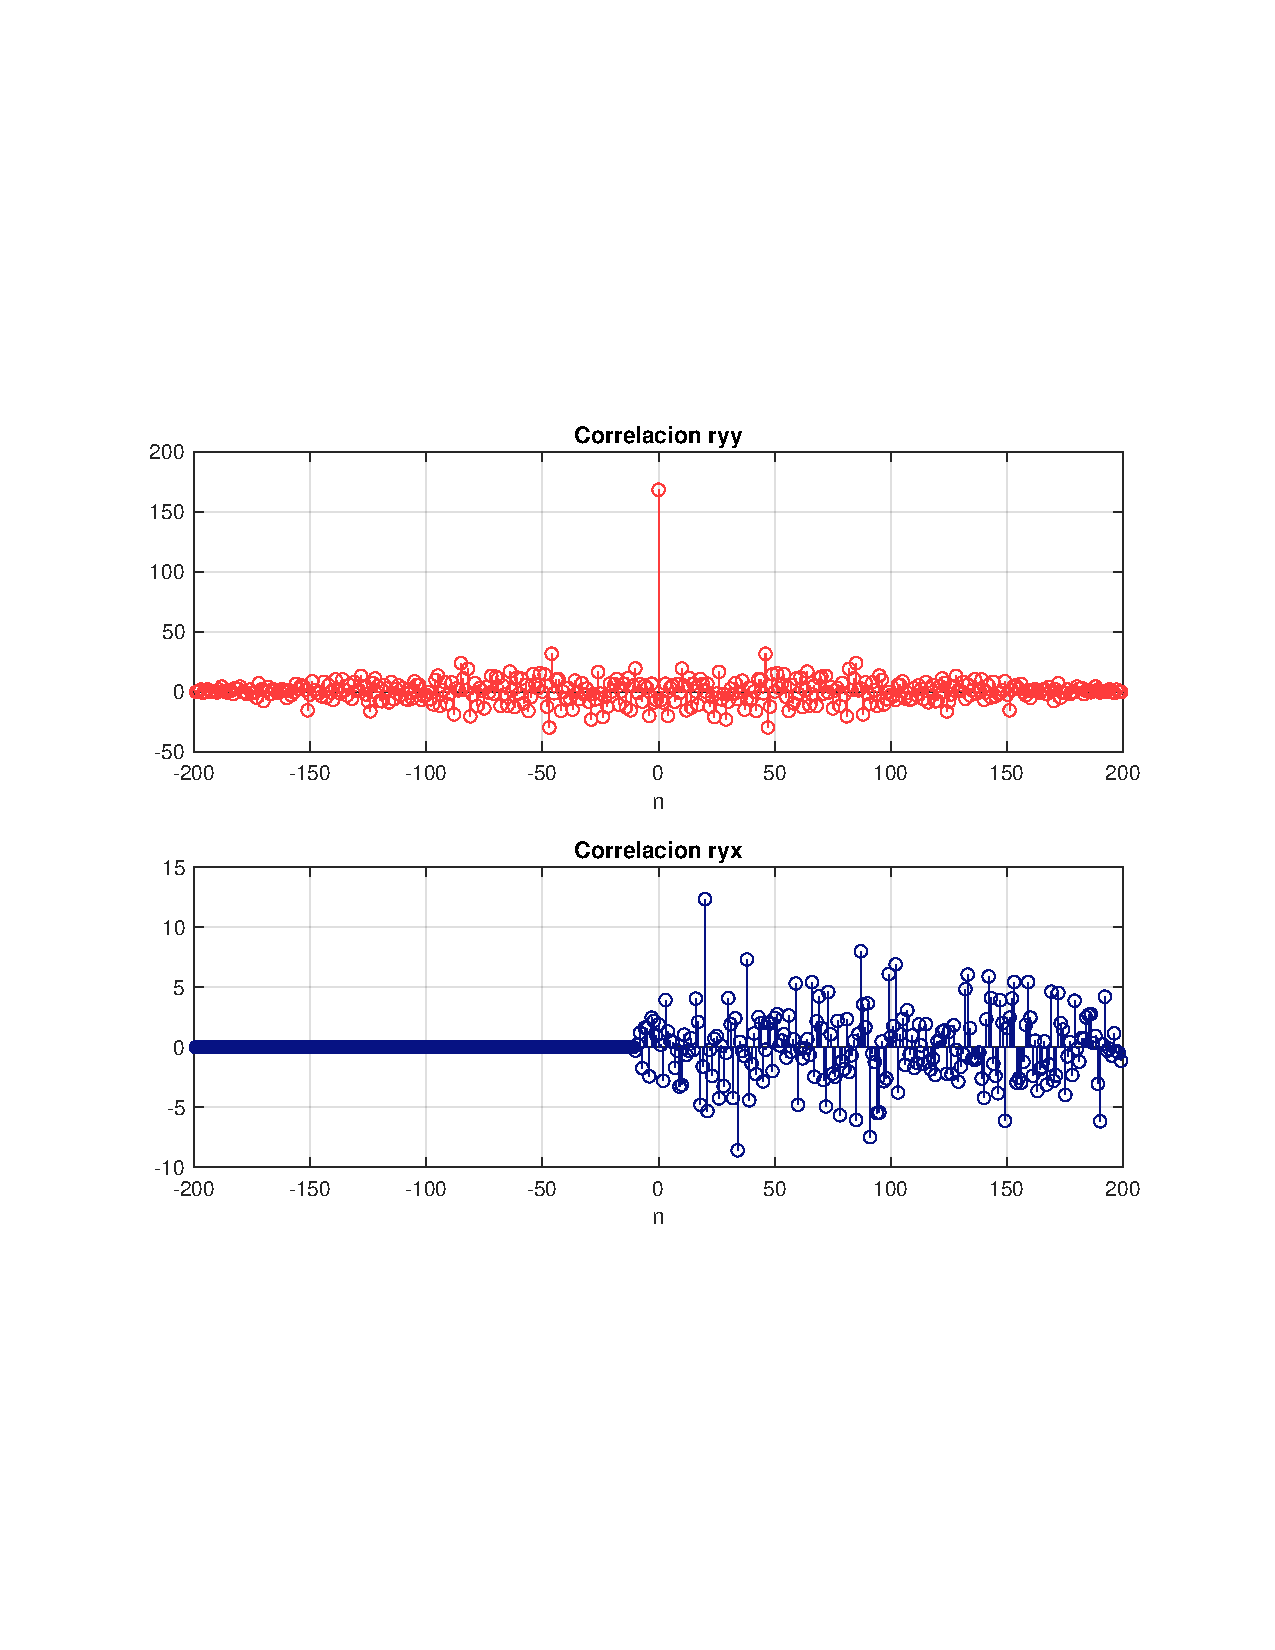
\includegraphics[width=0.6\textwidth,clip, trim = {2cm 7.0cm 2.2cm 7.0cm}]{../imgs/4_radar_d_1_corre.pdf}
			\caption{Correlación ryy e ryx de la situación anterior}
			\label{fig:radar_d_1_corre}
		\end{figure}
		
		Siguiendo con la misma tónica que el punto anterior, ahora con un SNR = 0.357 \textit{dB}, aun es posible determinar el retardo de la señal a partir del peak de la correlación. Sin embargo, ahora empiezan a aparecer peaks secundarios importantes que hacen especular que si se sigue aumentando, esta estimación podría empezar a ser imprecisa.
		
		\subsection{Simulación con 10 secuencias de Barker}
			\begin{figure}[H]
			\center
			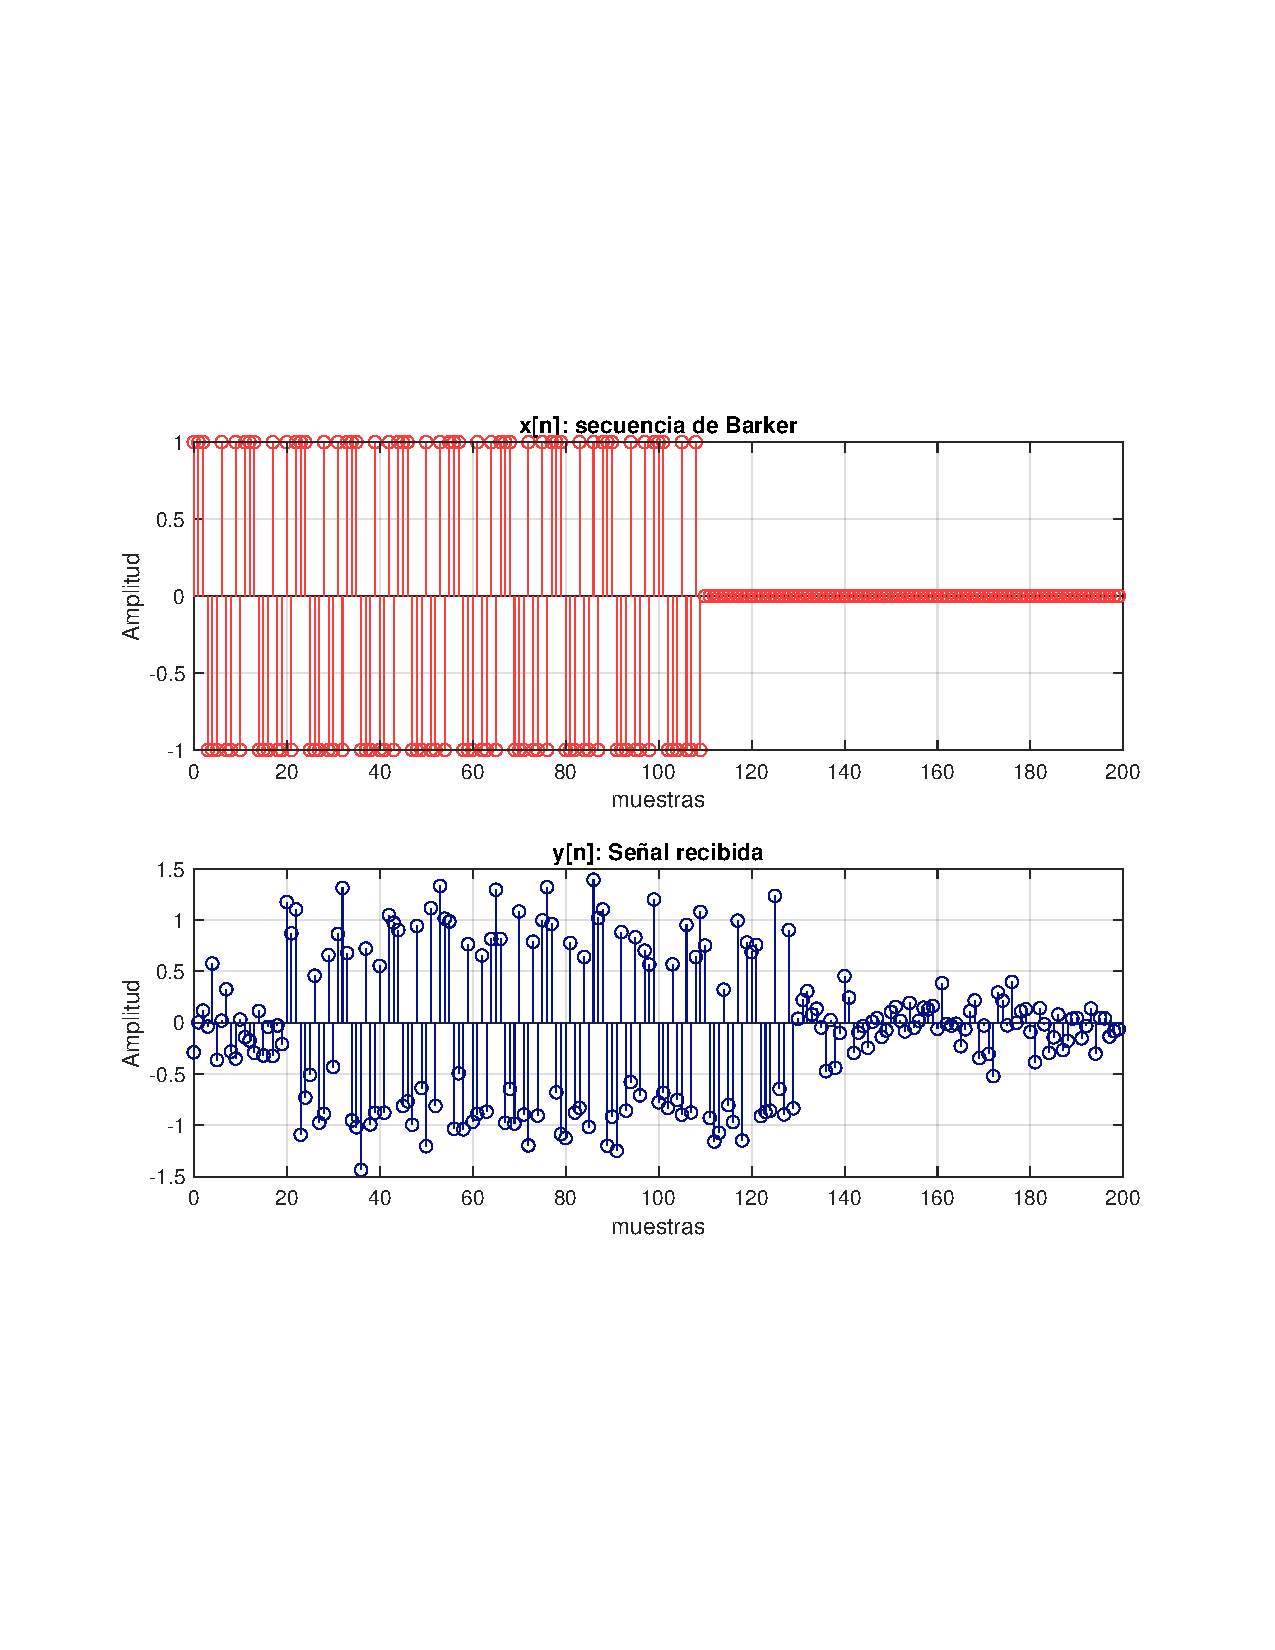
\includegraphics[width=0.6\textwidth,clip, trim = {2cm 7.0cm 2.2cm 7.0cm}]{../imgs/4_radar_e_signal.pdf}
			\caption{Simulación de la situación}
			\label{fig:radar_e_signal}
		\end{figure}
		
		\begin{figure}[H]
			\center
			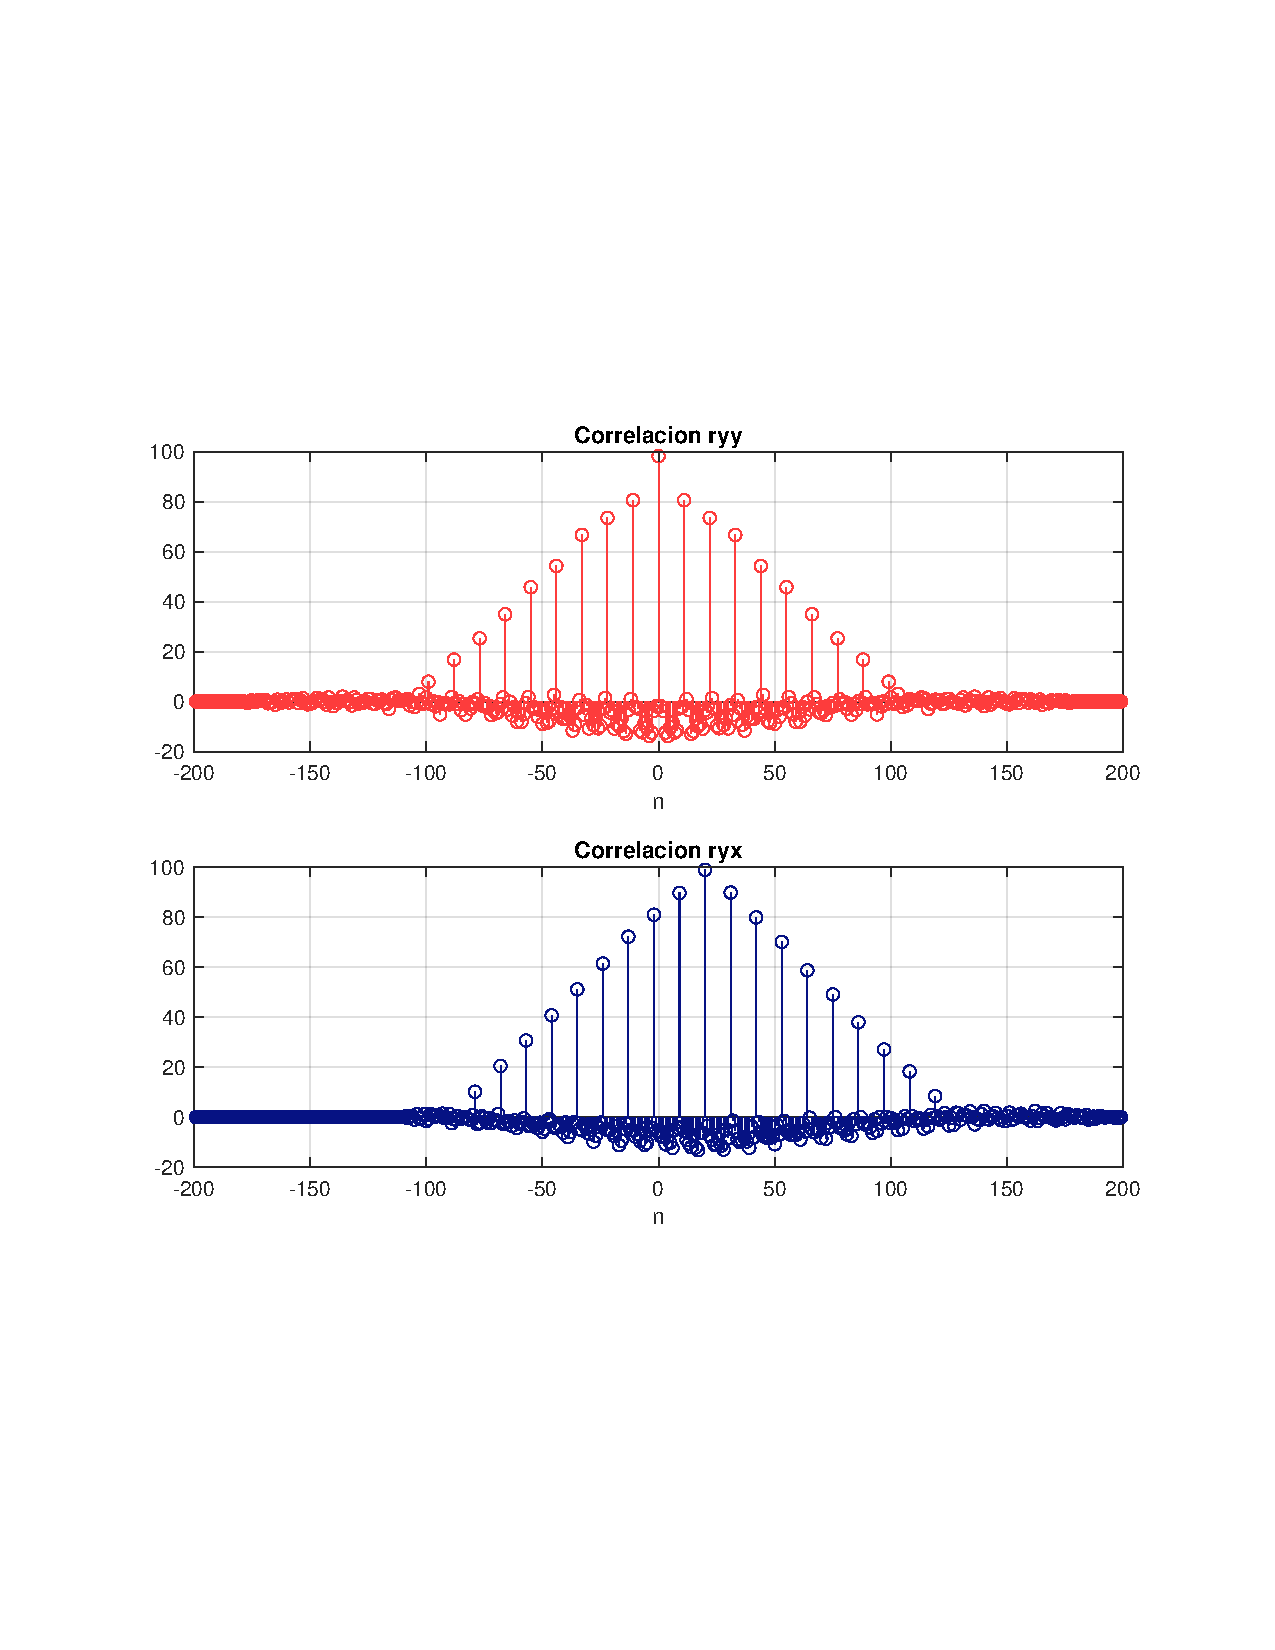
\includegraphics[width=0.6\textwidth,clip, trim = {2cm 7.0cm 2.2cm 7.0cm}]{../imgs/4_radar_e_corre.pdf}
			\caption{Correlación ryy e ryx de la situación anterior}
			\label{fig:radar_e_corre}
		\end{figure}
		
		Note que para esta caso, con diez secuencias de barker continuas, la estimación de D no ha cambiado, se tiene un peak central el cual corresponde al valor esperado, pero ahora es de una \textit{potencia mayor}, también aparecen bandas latearles al peak, que corresponden al desfase temporal entre los pulsos que son enviados. Para este caso, se tiene una mejor resistencia al ruido, teniendo un valor de SNR $\approx$ 10 \textit{dB}.

\end{document}
